\begin{center}


\includegraphics[width=0.3\textwidth]{assets/img/general/upc-logo.png}

\vspace{1cm}

{\LARGE \textbf{Univerisdad Peruana de Ciencias Aplicadas}}\\

\vspace{1cm}

{\LARGE Ingeniería de Software}\\

\vspace{1cm}

{\large 1ACC0238 | Fundamentos de Arquitectura de Software}\\

\vspace{0.5cm}

{\large NRC: 7944}\\

\vspace{0.5cm}

{\large Periodo: 202610}\\

\vspace{1.5cm}

{\LARGE \textbf{Informe del Trabajo Final}}\\

\vspace{1.25cm}

{\large Startup: HampCoders}\\

\vspace{0.5cm}

{\large Producto: Glottia}\\

\vspace{1.25cm}

Ethan Matias Aliaga Aguirre\\

\vspace{0.25cm}

Leandro Saul Contreras López\\

\vspace{0.25cm}

Italo Ludwing Sanchez Manrique\\

\vspace{0.25cm}

Ivo Marcelo Machado Bracamonte\\

\vspace{0.25cm}

Cesar Arostegui Alzamora\\

\vspace{1cm}

Noviembre 2025

\end{center}

\newpage
\tableofcontents
\newpage

\section{Registro de Versiones del
Informe}\label{report__01-registro-versiones.md__registro-de-versiones-del-informe}

{\def\LTcaptype{none} % do not increment counter
\begin{longtable}[]{@{}
  >{\raggedright\arraybackslash}p{(\linewidth - 6\tabcolsep) * \real{0.1636}}
  >{\raggedright\arraybackslash}p{(\linewidth - 6\tabcolsep) * \real{0.1273}}
  >{\raggedright\arraybackslash}p{(\linewidth - 6\tabcolsep) * \real{0.2000}}
  >{\raggedright\arraybackslash}p{(\linewidth - 6\tabcolsep) * \real{0.5091}}@{}}
\toprule\noalign{}
\begin{minipage}[b]{\linewidth}\raggedright
Versión
\end{minipage} & \begin{minipage}[b]{\linewidth}\raggedright
Fecha
\end{minipage} & \begin{minipage}[b]{\linewidth}\raggedright
Autor(es)
\end{minipage} & \begin{minipage}[b]{\linewidth}\raggedright
Descripción de modificación
\end{minipage} \\
\midrule\noalign{}
\endhead
\bottomrule\noalign{}
\endlastfoot
\textbf{TB1} & 06/04/2026 & \textbf{Ethan Matías Aliaga Aguirre} &
Establecer estructura principal para el informe del proyecto \\
\textbf{TB1} & 07/04/2026 & \textbf{Ethan Matías Aliaga Aguirre} &
Redactar primera versión del Capítulo I \\
\textbf{TB1} & 07/04/2026 & \textbf{Ethan Matías Aliaga Aguirre} &
Redactar Startup Profile \\
\textbf{TB1} & 07/04/2026 & \textbf{Ethan Matías Aliaga Aguirre} &
Redactar Solution Profile \\
\textbf{TB1} & 07/04/2026 & \textbf{Ethan Matías Aliaga Aguirre} &
Redactar tabla base para colocar nombres de los integrantes \\
\textbf{TB1} & 13/04/2026 & \textbf{Ethan Matías Aliaga Aguirre} &
Ajustar segmentos objetivos \\
\textbf{TB1} & 13/04/2026 & \textbf{Cesar Augusto Arostegui Alzamora} &
Añadio To-Be Scenario Mapping y realización de entrevistas \\
\textbf{TB1} & 15/04/2026 & \textbf{Ethan Matias Aliaga Aguirre} &
Corregir el formato del documento \\
\textbf{TB1} & 15/04/2026 & \textbf{Cesar Augusto Arostegui Alzamora} &
Realiza el User Task Matrix y su respectivo análisis \\
\textbf{TB1} & 18/04/2026 & \textbf{Cesar Augusto Arostegui Alzamora} &
Añadir el registro de entrevistas para los 2 segmentos objetivos y
análisis de las entrevistas \\
\textbf{TB1} & 18/04/2026 & \textbf{Sánchez Manrique, Italo Ludwing} &
Elaboración del Impact Map para definir objetivos de negocio y
alineación de funcionalidades \\
\textbf{TB1} & 18/04/2026 & \textbf{Sánchez Manrique, Italo Ludwing} &
Análisis de competidores para identificar oportunidades y diferenciación
del producto \\
\textbf{TB1} & 18/04/2026 & \textbf{Sánchez Manrique, Italo Ludwing} &
Desarrollo del Customer Journey Map (As-Is) para identificar problemas
actuales del usuario \\
\textbf{TB1} & 18/04/2026 & \textbf{Sánchez Manrique, Italo Ludwing} &
Apoyo en la realización y análisis de entrevistas a usuarios \\
\textbf{TB1} & 18/04/2026 & \textbf{Sánchez Manrique, Italo Ludwing} &
Creación y priorización del Product Backlog basado en valor de
negocio \\
\end{longtable}
}

\newpage

\subsection{Project Report Collaboration
Insights}\label{report__02-collaboration-insights.md__project-report-collaboration-insights}

\textbf{Enlace de la organización del proyecto} -
\href{https://github.com/Hampcoders-Fundamentos}{Organización GitHub:
Hampcoders-Fundamentos} -
\href{https://github.com/Hampcoders-Fundamentos/project-document.git}{Repositorio
GitHub: Hampcoders-Fundamentos-documento}

\textbf{Insights del TB1}

\pandocbounded{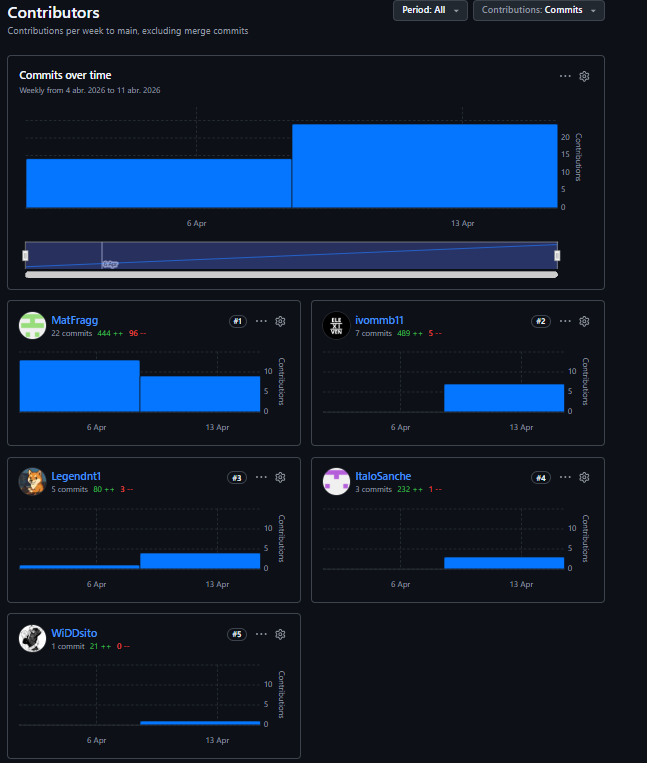
\includegraphics[keepaspectratio]{assets/img/cap2/Insgith-1.png}}

\newpage

\footnotesize

\section{Student
Outcome}\label{report__04-student-outcome.md__student-outcome}

{\def\LTcaptype{none} % do not increment counter
\begin{longtable}[]{@{}
  >{\raggedright\arraybackslash}p{(\linewidth - 4\tabcolsep) * \real{0.3704}}
  >{\raggedright\arraybackslash}p{(\linewidth - 4\tabcolsep) * \real{0.3704}}
  >{\raggedright\arraybackslash}p{(\linewidth - 4\tabcolsep) * \real{0.2593}}@{}}
\toprule\noalign{}
\begin{minipage}[b]{\linewidth}\raggedright
Criterio específico
\end{minipage} & \begin{minipage}[b]{\linewidth}\raggedright
Acciones realizadas
\end{minipage} & \begin{minipage}[b]{\linewidth}\raggedright
Conclusiones
\end{minipage} \\
\midrule\noalign{}
\endhead
\bottomrule\noalign{}
\endlastfoot
Actualiza conceptos y conocimientos necesarios para su desarrollo
profesional y en especial para su proyecto en soluciones de software. &
\textbf{Integrante 1:} Ethan Aliaga Aguirre ────────────────────────── -
TB1: En esta entrega pude actualizar conceptos relacionados a la
metodología Lean UX para realizar la definición del Problem Statement,
alcances y limites de nuestro proyecto. \textbf{Integrante 2:} Cesar
Augusto Arostegui Alzamora ────────────────────────── - TB1: Durante las
fases iniciales, se elaboraron los diagramas To-Be Scenario Mapping, se
estructuró el User Task Matrix y se ejecutó un análisis detallado y
estadístico de las entrevistas, aplicando directamente los principios de
la metodología Lean UX para recopilar requerimientos.
────────────────────────── \textbf{Integrante 3:} Italo Ludwing Sánchez
Manrique,────────────────────────── - TB1: Investigué y apliqué
herramientas y metodologías clave como User Persona, Customer Journey
Map (As-Is), Impact Map y análisis de competidores para comprender el
problema y definir la propuesta de valor del proyecto. Asimismo, aprendí
a estructurar y organizar un Product Backlog inicial basado en historias
de usuario orientadas al valor de negocio -
──────────────────────────\textbf{Integrante 4:} Nombre Apellido
────────────────────────── - TB1: .Descripción breve \textbf{Integrante
5:} Nombre Apellido ───────────────────────── - TB1: Descripción breve &
Conclusión\ldots{} \\
Reconoce la necesidad del aprendizaje permanente para el desempeño
profesional y el desarrollo de proyectos en soluciones de software. &
\textbf{Integrante 1:} Ethan Aliaga Aguirre ────────────────────────── -
TB1: Con el objetivo del desarrollo de este trabajo, sentí la necesidad
de investigar mucho más a fondo sobre algunos conceptos aplicados para
el desarrollo de las entrevistas para poder entender y analizar mejor
las necesidades de nuestros posibles usuarios.
──────────────────────────\textbf{Integrante 2:} Cesar Augusto Arostegui
Alzamora ────────────────────────── - TB1:La labor de conciliar dos
segmentos objetivos muy distintos demandó investigar temas fuera del
ámbito netamente técnico, requiriendo el estudio de modelos de
rentabilidad de negocios (casos B2B) y la psicología del comportamiento
y frustraciones de los estudiantes. - TB2: Descripción breve
──────────────────────────\textbf{Integrante 3:} Italo Ludwing Sánchez
Manrique,────────────────────────── - TB1: Durante el desarrollo del
proyecto identifiqué la necesidad de adquirir nuevos conocimientos en
metodologías UX, investigación de usuarios y herramientas de análisis
como Impact Mapping y benchmarking, lo que me permitió mejorar la
definición del problema y la solución propuesta.
──────────────────────────\textbf{Integrante 4:} Nombre Apellido
────────────────────────── - TB1: Descripción breve - TB2: Descripción
breve \textbf{Integrante 5:} Nombre Apellido ──────────────────────────
- TB1: Descripción breve & En el presente trabajo, el equipo de
Hampcoders ha dejado en evidencia la actualización y aplicación práctica
de nuevos marcos de trabajo analíticos, logrando traducir de forma
precisa los hallazgos cualitativos del mercado en características y
requerimientos arquitectónicos sólidos para el software. \\
\end{longtable}
}

\normalsize

\newpage

\section{Capítulo I:
Introducción}\label{report__10-cap1-introduccion.md__capuxedtulo-i-introducciuxf3n}

En este capítulo el equipo presenta el contexto general del proyecto que
se trabajará durante el ciclo, incluyendo la descripción de la startup,
los problemas identificados y la solución propuesta. En adición, se
especifica el proceso de Lean UX utilizado para la validación del
producto y segmentos objetivos.

\subsection{1.1. Startup
Profile}\label{report__10-cap1-introduccion.md__startup-profile}

En esta sección el equipo describe el perfil de la startup, el propósito
y el perfil de los integrantes.

\subsubsection{1.1.1. Descripción de la
Startup}\label{report__10-cap1-introduccion.md__descripciuxf3n-de-la-startup}

En Hampcoders creemos en crear tecnología que realmente tenga impacto.
Usamos herramientas open-source para desarrollar soluciones digitales
pensadas en problemas reales del día a día. Desde el inicio tuvimos
claro que no se trata solo de programar, sino de ayudar a las personas y
a los emprendedores a trabajar mejor, simplificando sus procesos y
dándoles herramientas útiles, prácticas y sin complicaciones.

Misión: Democratizar la tecnología open-source para resolver los
problemas reales de personas y emprendedores.

Visión: Ser el motor tecnológico detrás de la próxima generación de
emprendedores exitosos, impulsados por el código abierto.

\subsubsection{1.1.2. Perfiles de Integrantes del
equipo}\label{report__10-cap1-introduccion.md__perfiles-de-integrantes-del-equipo}

\begin{minipage}{0.3\textwidth}

\includegraphics[width=\linewidth]{assets/img/cap1/team/ethan.png}
\end{minipage}
\hfill
\begin{minipage}{0.65\textwidth}

\textbf{Ethan Matias Aliaga Aguirre} \\
Código: U202318323  

Soy Ethan Matias Aliaga Aguirre, estudiante de 7mo ciclo de Ingeniería de Software en la UPC, sede San Miguel. Me caracterizo por mi compromiso, responsabilidad, habilidad para trabajar en equipo y comunicación. Mis conocimientos incluyen arquitectura de software y desarrollo de APIs. Además, tengo experiencia en el uso de herramientas como Photoshop, Filmora y Vegas Studio, lo que me permite aportar con soluciones creativas y técnicas en mis proyectos. Estoy comprometido con mi crecimiento personal y profesional, siempre buscando aprender y mejorar en cada oportunidad que se presente.
\end{minipage}

\vspace{1cm}

\begin{center}\rule{0.5\linewidth}{0.5pt}\end{center}

\begin{minipage}{0.3\textwidth}

\includegraphics[width=\linewidth]{assets/img/cap1/team/leandro.png}
\end{minipage}
\hfill
\begin{minipage}{0.65\textwidth}

\textbf{Leandro Saúl Contreras López} \\
**Código:** U20231E215

Mucho gusto, soy Leandro Contreras, estudiante de la carrera de Ingeniería de Software en la UPC, sede San Miguel. Tengo 19 años y estoy cursando el sexto ciclo académico. Me considero una persona adaptativa, perseverante y comprometida con lo que me propongo. En este proyecto tengo como objetivo buscar múltiples soluciones que beneficien a todo el grupo. Por experiencia propia, suelo trabajar de manera colaborativa y eficaz. Al terminar la carrera de ingeniería, me gustaría estudiar una segunda carrera: Gastronomía y Gestión Culinaria.
\end{minipage}

\vspace{1cm}

{\def\LTcaptype{none} % do not increment counter
\begin{longtable}[]{@{}
  >{\raggedright\arraybackslash}p{(\linewidth - 0\tabcolsep) * \real{0.0556}}@{}}
\toprule\noalign{}
\endhead
\bottomrule\noalign{}
\endlastfoot
 \\
\textbf{Ivo Marcelo Machado Bracamonte} \textbackslash{}
\textbf{Código:} U20231C368 \\
Mi nombre es Ivo Machado, tengo 19 años y soy estudiante del sexto ciclo
de Ingeniería de Software en la UPC. Me caracterizo por mi mentalidad
resiliente, ya que no me rindo con facilidad y no le tengo miedo al
error. Tengo empatía con los demás, disfruto resolver problemas y busco
mejorar constantemente en lo que hago. Poseo conocimientos en lenguajes
de programación como C++, Java y Python, así como en HTML, CSS y
JavaScript. Además, domino el inglés y tengo conocimientos de
portugués. \\
\textbackslash end\{minipage\} \\
\vspace{1cm} \\
\end{longtable}
}

\begin{minipage}{0.3\textwidth}

\includegraphics[width=\linewidth]{assets/img/cap1/team/Italo-foto.jpeg}
\end{minipage}
\hfill
\begin{minipage}{0.65\textwidth}

\textbf{Italo Ludwing Sanchez Manrique} \\
Código: U202316967  

Mi nombre es Italo Ludwing Sanchez Manrique, soy estudiante de Ingeniería de Software en la UPC. Tengo 19 años y actualmente curso el sexto ciclo académico. Destaco por mi perseverancia, tolerancia y compromiso con mis metas. En este proyecto, mi objetivo es buscar soluciones que beneficien al grupo, ya que tengo experiencia trabajando de forma proactiva y colaborativa. Además, poseo sólidos conocimientos en lenguajes de programación como Java y C++.
\end{minipage}

\vspace{1cm}

\subsection{}\label{report__10-cap1-introduccion.md__section}

\begin{minipage}{0.3\textwidth}
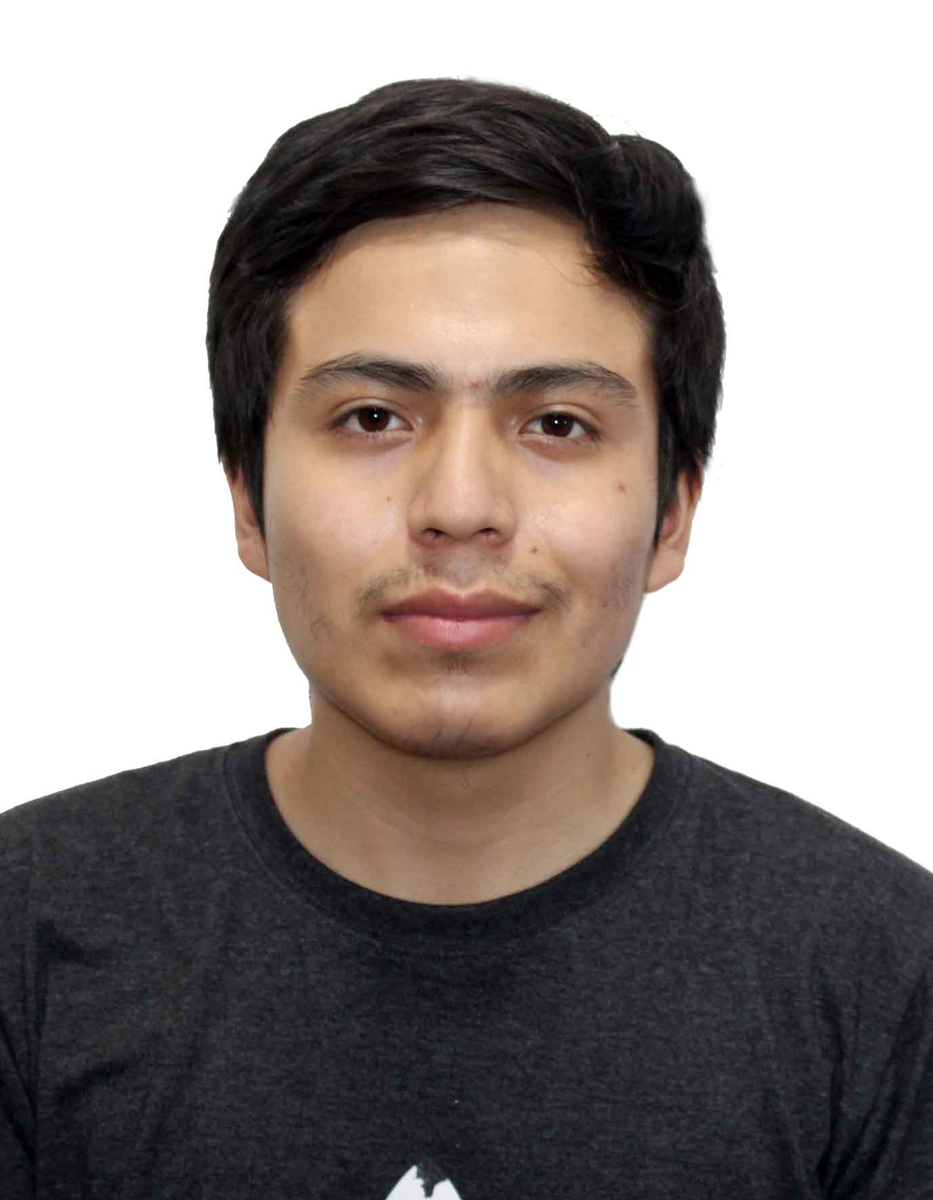
\includegraphics[width=\linewidth]{assets/img/cap1/team/cesar.png}
\end{minipage}
\hfill
\begin{minipage}{0.65\textwidth}

\textbf{César Augusto Arostegui Alzamora} \\
**Código:** U202114548

Soy César Augusto, estudiante de Ingeniería de Software. Actualmente tengo 21 años. Mi lenguaje de programación más utilizado y favorito es TypeScript. Actualmente me encuentro desarrollando habilidades en áreas como DevOps y frameworks de desarrollo móvil.
\end{minipage}

\vspace{1cm}

\subsection{1.2. Solution
Profile}\label{report__10-cap1-introduccion.md__solution-profile}

En esta sección el equipo describe el perfil de la solución, inluyendo
el análisis mediante la metodología Lean UX

\subsubsection{1.2.1 Nombre del
producto}\label{report__10-cap1-introduccion.md__nombre-del-producto}

Tras la pandemia en Perú, notamos una oportunidad al juntar tres
problemas actuales. Por una parte, muchos jóvenes tienen dificultades
para relacionarse cara a cara, mientras que miles de estudiantes de
idiomas se quedan en la teoría por falta de espacios para conversar. A
esto se le suma que los pequeños negocios, como cafeterías, buscan
constantemente nuevas formas de generar tráfico de clientes.

Así nace Glottia, una iniciativa para incentivar la práctica presencial
de idiomas. Lo que hacemos es conectar a personas que quieren soltarse
al hablar con restaurantes y cafés locales, dándoles a los usuarios un
lugar cómodo para practicar y a los negocios un flujo constante de
público.

\subsubsection{1.2.2 Antecedentes y
problemática}\label{report__10-cap1-introduccion.md__antecedentes-y-problemuxe1tica}

Para detallar los antecedentes de la solución y describir la
problemática de manera estructurada, se utilizó la técnica de las 5W +
2H.

\begin{longtable}{|p{6cm}|p{9cm}|}
\hline
\textbf{Pregunta} & \textbf{Respuesta} \\
\hline

¿Qué (What) - ¿Cuál es el problema?
& Jóvenes interesados en aprender idiomas no pueden encontrar espacios sociales y constantes para practicar un idioma con conversación real. \\
\hline

¿Quién (Who) - ¿Quiénes son los beneficiarios?
& Jóvenes adultos de 18 a 35 años, universitarios, egresados y profesionales que buscan mejorar su fluidez en idiomas. \\
\hline

¿Cuándo (When) - ¿Cuándo se origina el problema?
& El problema ocurre cuando una persona quiere practicar un idioma en un entorno real y no encuentra un espacio apropiado y flexible para hacerlo. \\
\hline

¿Por qué (Why) - ¿Por qué se origina el problema?
& Se origina debido al alto costo de cursos conversacionales de academias y escasez de espacios organizados para practicar idiomas de forma social. \\
\hline

¿Dónde (Where) - ¿Dónde ocurre el problema?
& Contextos urbanos donde no existen espacios accesibles para la práctica activa de idiomas. \\
\hline

¿Cómo (How) - ¿Cómo se origina el problema?
& Se origina por la falta de integración entre personas con interés en idiomas y espacios adecuados, además de la ausencia de plataformas que combinen interacción social y presencialidad. \\
\hline

¿Cuánto (How much) - ¿Cuánto dinero está implicado?
& Los cursos enfocados en conversación en academias y centros de idiomas en Lima suelen oscilar entre 100 y 250 soles mensuales, variando según duración y frecuencia. \\
\hline

\end{longtable}

\subsubsection{1.2.3 Lean UX
Process}\label{report__10-cap1-introduccion.md__lean-ux-process}

En esta sección el equipo aplica la metodología Lean UX para definir el
problema, las suposiciones y las hipotesis.

\paragraph{1.2.3.1 Lean UX Problem
Statement}\label{report__10-cap1-introduccion.md__lean-ux-problem-statement}

Nuestra plataforma tiene como propósito brindar oportunidades de
práctica conversacional en distintos idiomas, eliminando barreras
económicas y geográficas. Buscamos que cualquier persona, sin importar
su ubicación o condición económica, pueda mejorar su fluidez y confianza
al comunicarse en otra lengua.

Hemos observado que los jóvenes adultos enfrentan cada vez mayores
obstáculos para acceder a prácticas lingüísticas constantes,
principalmente debido al alto costo de las academias tradicionales o la
ausencia de espacios organizados cerca de sus zonas de residencia o
estudio.

Ante este desafío, surge la pregunta: ¿Cómo podemos proporcionar
opciones accesibles (económicamente y geográficamente) para practicar
idiomas sin depender de instituciones costosas o ubicaciones limitadas?

\paragraph{1.2.3.2 Lean UX
Assumptions}\label{report__10-cap1-introduccion.md__lean-ux-assumptions}

\paragraph{Business
Outcomes:}\label{report__10-cap1-introduccion.md__business-outcomes}

\textbf{Creemos que nuestros usuarios necesitan} una plataforma que
conecte la práctica de idiomas en espacios reales con negocios que
necesitan una demanda más alta, mediante la organización de encuentros
grupales que generen un valor tanto para los aprendices como para los
negocios.

\textbf{Estas necesidades se pueden resolver mediante el} desarrollo de
una plataforma que facilite la reserva y organización de espacios en
cafeterías para encuentros grupales de prácticas de idiomas. Para las
cafeterías, esta plataforma debe contar con funcionalidades que
automaticen y simplifiquen la gestión de los espacios y para los
aprendices, la plataforma debe ofrecer herramientas qu faciliten la
búsqueda de encuentros.

\textbf{Nuestros clientes iniciales son} dueños de cafeterias que buscan
mejorar sus ingresos y clientes concurrentes, a su vez, aprendices de
idiomas que desean una experiencia más real, dínamica y efectiva para
alcanzar sus objetivos.

\textbf{El valor \#1 que los clientes quiere de nuestro servicio es}
reservar espacios en cafeterías para iniciar conversaciones grupales
donde pueda practicar y aprender. Los dueños de cafetería buscan
impulsar sus ventas y volverse un local mas concurrente, confiable y
amigable.

\textbf{El cliente también puede obtener estos beneficios adicionales}
como descuentos y promociones en las cafaterías afiliadas, incentivando
particiación y generando fidelización. Por parte de las cafeterías,
obtendrán un incremento del flujo de clientes y tendrán mayor consumo en
horarios de baja demanda.

\textbf{Vamos a adquirir la mayoría de los clientes a través de}
afiliaciones a cafeterías potenciales que deseen promover sus espacios
para la práctica de idiomas grupales. Promover la práctica de idiomas
cara a cara siendo promocionadas en centros de estudios de idiomas para
generar interración en nuestro público objetivo.

\textbf{Haremos dinero a través de} un modelo de suscripciones y
afiliaciones adaptado a la necesidad del segmento objetivo y ofreciendo
funcionalidades especiales.

\textbf{Nuestra competencia de mercado serán} plataformas digitales de
aprendizaje de idiomas como DuoLingo, Tandem, HelloTalk las cuales
ofrecen la práctica de idiomas mediante chat, audio y video. También,
establecimientos físicos que son una competencia indirecta como
Británico, ICPNA, Starbucks.

\textbf{Los venceremos debido a} que nuestra solución ofrece una
combinación entre lo digital y lo presencial, facilitando la práctica de
idiomas mediante la encuentros organizados en cafeterías que ofrecen
espacios tranquilos, permitiendo una experiencia interactiva, accesible
y social en comparación a las alternativas tradicionales.

\textbf{Nuestro mayor riesgo de producto es} que los dueños de
cafeterías no ofrezcan sus espacios exclusivamente a reservar de su
local. Asimismo, temen desconfiar que los aprendices no realicen
consumos dentro del local. Finalmente; no ser de suficiente de
relevancia para impulsar su negocio.

\textbf{Resolveremos esto a través de} pruebas gratuitas y promociones a
los aprendices para que consuman en los locales y al mismo tiempo
recomendarlos, lo que permite desarrollar una economía estable, mejor
oferta/demanda y mejor rating en la plataforma.

\textbf{Qué otras suposiciones tenemos que, de probarse falsas, pueden
causar que nuestro proyecto fracase:}

\begin{itemize}
\item
  Los dueños de las cafeterías estarán dispuestos a ofrecer sus espacios
  a disponibilidad de los grupos de aprendices que hagan reservas por
  encima de cualquier otro cliente que desee usar el espacio
  espontáneamente.
\item
  Creemos que los aprendices prefieren un modelo de práctica del habla y
  escucha de un idioma distinto en grupos presenciales de práctica en un
  establecimiento.
\item
  Creemos que los aprendices tomarán las promociones y descuentos como
  motivación para realizar encuentros y consumir en las cafeterias de
  manera que les permitan impulsar las ganancias y mejorar el
  reconocimiento de los locales afiliados.
\end{itemize}

\paragraph{User
Outcomes:}\label{report__10-cap1-introduccion.md__user-outcomes}

\begin{enumerate}
\def\labelenumi{\arabic{enumi}.}
\tightlist
\item
  ¿Quien será el usuario?

  \begin{itemize}
  \tightlist
  \item
    Glottia incluirá dos usuarios: los aprendices; quienes buscan tener
    encuentros grupales en locales agradables para estudiar, practicar y
    mejorar sus habilidades en distintos idiomas. Y los dueños de
    cafeterías; que aspiran a mejorar sus ganancias y ser reconocidos en
    el mercado.
  \end{itemize}
\item
  ¿Donde encaja nuestro producto en su trabajo o vida?

  \begin{itemize}
  \tightlist
  \item
    Ambos usuarios pueden utilizarlo en sus quehaceres diarios o
    jornadas habituales, pues los dueños de cafetería querrán tener
    conocimiento acerca de estadísticas de su local, sea en ganancias o
    calificaciones. Del mismo modo, los aprendices, pueden realizar
    reservas durante el día en el horario más adecuado para ellos y no
    perderse de sus lecciones.
  \end{itemize}
\item
  ¿Qué problemas busca resolver nuestro producto?

  \begin{itemize}
  \tightlist
  \item
    Buscamos desconectar la brecha de incomodidad y monotonía por parte
    de los aprendices al sacarlos de su zona de confort (generadas por
    las clases remotas) para brindarles una alternativa más dinámica y
    eficiente gracias a reuniones grupales en locales de cafeterías.
    Además planeamos brindar una plataforma interactiva hacia los dueños
    de locales donde podrán organizar, administrar y medir sus
    indicadores clave de desempeño (KPI's)
  \end{itemize}
\item
  ¿Cuándo y Cómo es usado nuestro producto?

  \begin{itemize}
  \tightlist
  \item
    Puede ser utilizado en cualquier momento del día -laboral- tanto por
    aprendices como locales para concretar reuniones o análisis (según
    el usuario) y generar una experiencia más colectiva y servicial.
    Ambos usuarios accederán a la aplicación mediante un dispositivo
    móvil
  \end{itemize}
\item
  ¿Que características son importantes?

  \begin{itemize}
  \tightlist
  \item
    Reserva y asignación de espacio en la cafetería seleccionada de
    preferencia.
  \item
    Interfaz intuitiva y minimalista para optimizar el flujo de
    navegación.
  \item
    Dashboard visual que muestren diferentes campos asociados a la
    administración del local.
  \item
    Recompensar a los usuarios con premios dentro de la aplicación para
    fomentar su uso con frecuencia.
  \end{itemize}
\item
  ¿Como debe comportarse y verse nuestro producto?

  \begin{itemize}
  \tightlist
  \item
    Incluir secciones personalizadas: Cada usuario debe visualizar
    diferentes interfaces acordes a sus necesidades y objetivos.
  \item
    Interfaz minimalista e intuitiva: Fundamental para crear una
    comunidad y permitir expandir la aplicación a mas usuarios que
    quieran aprovechar de esta solución.
  \end{itemize}
\end{enumerate}

\paragraph{1.2.3.3 Lean UX
Hypothesis}\label{report__10-cap1-introduccion.md__lean-ux-hypothesis}

\textbf{Creemos que} los aprendices estarán interesados en utilizar
Glottia porque les permite mejorar sus habilidades lingüisticas al tener
reuniones presenciales grupales.

\textbf{Sabremos que} los aprendices encontrarán valor en la plataforma
\textbf{cuando veamos} que el 50\% de los aprendices comiencen a
realizar reuniones en un nivel avanzado o nativo dentro de la
aplicación.

\textbf{Cremos que} incluir examenés o pruebas simuladas dentro de la
aplicación fomentará un dominio en su idioma preferido

\textbf{Sabremos que} los aprendices estarán mejorando sus habilidades
\textbf{cuando veamos} que el 40\% de los aprendices se encuentran
rindiendo pruebas o examenes dentro de la aplicación además de cumplir
con sus reuniones grupales.

\textbf{Creemos que} los dueños de cafeterías de Lima estarán
interesados en Glottia porque les permite aumentar las ganancias en
horarios de baja demanda.

\textbf{Sabremos que} los dueños de cafeterías van a encontrar valor en
la plataforma \textbf{cuando veamos} que el 60\% de las cafeterías se
encuentren afiliadas a la aplicación y utilicen diariamente sus
funcionalidades para gestionar sus espacios.

\textbf{Creemos que} al agregar descuentos en las cafeterías por la
participación en encuentros de práctica de idiomas lograremos
fidelización de parte de los usuarios hacia Glottia.

\textbf{Sabremos que} los descuentos agregados son efectivos
\textbf{cuando veamos} que la tasa de usuarios recurrentes y de
participación en encuentros aumente en un 20\% en 6 semanas.

\paragraph{1.2.3.4 Lean UX
Canvas}\label{report__10-cap1-introduccion.md__lean-ux-canvas}

\pandocbounded{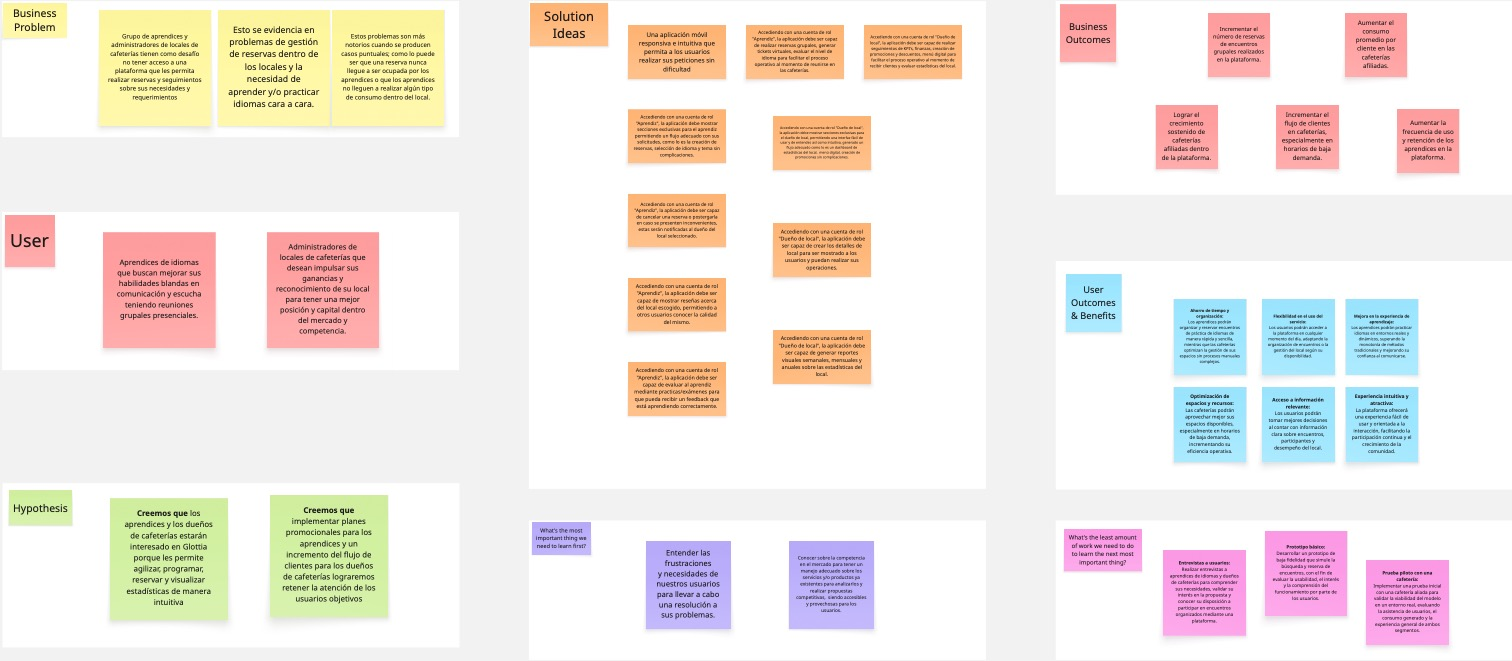
\includegraphics[keepaspectratio]{assets/img/cap1/canvas/lean-ux-canvas-Glottia.jpg}}

\subsection{1.3 Segmentos
objetivo}\label{report__10-cap1-introduccion.md__segmentos-objetivo}

\textbf{Segmento objetivo \#1: Usuarios aprendices de idiomas}

\paragraph{Aspectos
demográficos:}\label{report__10-cap1-introduccion.md__aspectos-demogruxe1ficos}

\begin{itemize}
\tightlist
\item
  Sexo: Masculino, femenino y no binario.
\item
  Edad: Entre 16 y 40 años (desde estudiantes de secundaria superior
  hasta jóvenes/adultos profesionales).
\item
  Nivel socioeconómico: Medio a medio-alto.
\end{itemize}

\paragraph{Aspectos
geográficos:}\label{report__10-cap1-introduccion.md__aspectos-geogruxe1ficos}

\begin{itemize}
\tightlist
\item
  Residen en áreas urbanas o metropolitanas con buena conectividad y
  vida cultural activa.
\item
  Se concentran en ciudades con alta población estudiantil, diversidad
  cultural o presencia de comunidades extranjeras.
\item
  Frecuentan espacios como universidades, bibliotecas, coworkings,
  cafeterías, bares, centros culturales y parques urbanos.
\end{itemize}

\paragraph{Aspectos
psicográficos:}\label{report__10-cap1-introduccion.md__aspectos-psicogruxe1ficos}

\begin{itemize}
\tightlist
\item
  Tienen motivación tanto académica/profesional (certificaciones,
  prácticas, empleabilidad) como social/personal (viajar, conocer
  culturas, socializar).
\item
  Buscan fluidez, vocabulario conversacional y confianza al hablar en un
  entorno real.
\item
  Valoran experiencias auténticas, accesibles y presenciales fuera de un
  aula tradicional.
\item
  Son curiosos, abiertos, sociables y dispuestos a salir de su zona de
  confort.
\end{itemize}

\begin{center}\rule{0.5\linewidth}{0.5pt}\end{center}

\textbf{Segmento objetivo \#2: Administradores que ofrecen su
establecimiento como punto de reunión}

\paragraph{Aspectos
demográficos:}\label{report__10-cap1-introduccion.md__aspectos-demogruxe1ficos-1}

\begin{itemize}
\tightlist
\item
  Perfil: Administradores, dueños o encargados de cafetería.
\item
  Tipo de negocio: Establecimientos con espacios adecuados para grupos
  pequeños o medianos (3 a 4 personas).
\item
  Ubicación: Zonas céntricas, estudiantiles o con alto tránsito de
  jóvenes/adultos interesados en socializar y aprender idiomas.
\end{itemize}

\paragraph{Aspectos
geográficos:}\label{report__10-cap1-introduccion.md__aspectos-geogruxe1ficos-1}

\begin{itemize}
\tightlist
\item
  Se encuentran en áreas urbanas y metropolitanas con vida cultural
  activa.
\item
  Están ubicados en distritos o barrios con alta concentración de
  estudiantes, profesionales jóvenes y comunidades extranjeras.
\item
  Sus locales suelen estar cerca de universidades, residencias
  estudiantiles, coworkings o zonas de ocio.
\end{itemize}

\paragraph{Aspectos
psicográficos:}\label{report__10-cap1-introduccion.md__aspectos-psicogruxe1ficos-1}

\begin{itemize}
\tightlist
\item
  Buscan atraer nuevos clientes mediante experiencias innovadoras.
\item
  Están interesados en diferenciar su local con propuestas culturales y
  sociales.
\item
  Valoran el posicionamiento digital y la visibilidad que les brinda la
  app.
\item
  Quieren generar mayor consumo en su establecimiento a través de las
  reuniones organizadas.
\item
  Desean fidelizar clientes al vincular su espacio con un ambiente
  inclusivo, cultural e internacional.
\end{itemize}

\newpage

\section{Capítulo II: Requirements \&
Analysis}\label{report__20-cap2-requirements-analysis.md__capuxedtulo-ii-requirements-analysis}

En este capítulo, el equipo recopila a información y requerimientos para
realizar analisis y proyectar la solución frente a los competidores
directos.

\subsection{2.1
Competidores}\label{report__20-cap2-requirements-analysis.md__competidores}

En esta sección se identifican y describen los principales competidores
de Glottia, considerando tanto competidores directos (plataformas de
intercambio de idiomas) como indirectos (plataformas de eventos
sociales).

\subsubsection{2.1.1 Análisis
Competitivo}\label{report__20-cap2-requirements-analysis.md__anuxe1lisis-competitivo}

\textbf{Competitive Analysis Landscape}

\paragraph{2.1.1.1 Objetivo del
análisis}\label{report__20-cap2-requirements-analysis.md__objetivo-del-anuxe1lisis}

{\def\LTcaptype{none} % do not increment counter
\begin{longtable}[]{@{}
  >{\raggedright\arraybackslash}p{(\linewidth - 2\tabcolsep) * \real{0.3333}}
  >{\raggedright\arraybackslash}p{(\linewidth - 2\tabcolsep) * \real{0.6667}}@{}}
\toprule\noalign{}
\begin{minipage}[b]{\linewidth}\raggedright
Plataforma
\end{minipage} & \begin{minipage}[b]{\linewidth}\raggedright
Objetivo del análisis
\end{minipage} \\
\midrule\noalign{}
\endhead
\bottomrule\noalign{}
\endlastfoot
Glottia & Identificar oportunidades de diferenciación mediante
experiencias presenciales y virtuales para la práctica de idiomas. \\
HelloTalk & Comprender su enfoque digital en aprendizaje. \\
Tandem & Analizar su comunidad global. \\
Meetup & Evaluar su modelo de eventos sociales. \\
\end{longtable}
}

\paragraph{2.1.1.2 Perfil
Overview}\label{report__20-cap2-requirements-analysis.md__perfil-overview}

{\def\LTcaptype{none} % do not increment counter
\begin{longtable}[]{@{}
  >{\raggedright\arraybackslash}p{(\linewidth - 2\tabcolsep) * \real{0.4583}}
  >{\raggedright\arraybackslash}p{(\linewidth - 2\tabcolsep) * \real{0.5417}}@{}}
\toprule\noalign{}
\begin{minipage}[b]{\linewidth}\raggedright
Plataforma
\end{minipage} & \begin{minipage}[b]{\linewidth}\raggedright
Descripción
\end{minipage} \\
\midrule\noalign{}
\endhead
\bottomrule\noalign{}
\endlastfoot
Glottia & Plataforma que conecta personas para practicar idiomas en
espacios físicos y virtuales. \\
HelloTalk & App de intercambio de idiomas con chat y correcciones. \\
Tandem & Plataforma de intercambio con hablantes nativos. \\
Meetup & Plataforma de organización de eventos sociales. \\
\end{longtable}
}

\paragraph{2.1.1.3 Ventaja
Competitiva}\label{report__20-cap2-requirements-analysis.md__ventaja-competitiva}

{\def\LTcaptype{none} % do not increment counter
\begin{longtable}[]{@{}
  >{\raggedright\arraybackslash}p{(\linewidth - 2\tabcolsep) * \real{0.4074}}
  >{\raggedright\arraybackslash}p{(\linewidth - 2\tabcolsep) * \real{0.5926}}@{}}
\toprule\noalign{}
\begin{minipage}[b]{\linewidth}\raggedright
Plataforma
\end{minipage} & \begin{minipage}[b]{\linewidth}\raggedright
Valor ofrecido
\end{minipage} \\
\midrule\noalign{}
\endhead
\bottomrule\noalign{}
\endlastfoot
Glottia & Experiencia híbrida (presencial + digital) y conexión
cultural. \\
HelloTalk & Corrección en tiempo real y herramientas integradas. \\
Tandem & Conexión global con hablantes nativos. \\
Meetup & Amplia red de eventos y usuarios. \\
\end{longtable}
}

\paragraph{2.1.1.4 Perfil de
Marketing}\label{report__20-cap2-requirements-analysis.md__perfil-de-marketing}

{\def\LTcaptype{none} % do not increment counter
\begin{longtable}[]{@{}
  >{\raggedright\arraybackslash}p{(\linewidth - 4\tabcolsep) * \real{0.1964}}
  >{\raggedright\arraybackslash}p{(\linewidth - 4\tabcolsep) * \real{0.3214}}
  >{\raggedright\arraybackslash}p{(\linewidth - 4\tabcolsep) * \real{0.4821}}@{}}
\toprule\noalign{}
\begin{minipage}[b]{\linewidth}\raggedright
Plataforma
\end{minipage} & \begin{minipage}[b]{\linewidth}\raggedright
Mercado objetivo
\end{minipage} & \begin{minipage}[b]{\linewidth}\raggedright
Estrategias de marketing
\end{minipage} \\
\midrule\noalign{}
\endhead
\bottomrule\noalign{}
\endlastfoot
Glottia & Jóvenes (16-40) y establecimientos & Redes sociales, alianzas
con locales, eventos \\
HelloTalk & Estudiantes de idiomas & Marketing digital, comunidad \\
Tandem & Usuarios globales & Marketing digital, app \\
Meetup & Público general & SEO, eventos, comunidades \\
\end{longtable}
}

\paragraph{2.1.1.4.5 Perfil de
Producto}\label{report__20-cap2-requirements-analysis.md__perfil-de-producto}

{\def\LTcaptype{none} % do not increment counter
\begin{longtable}[]{@{}
  >{\raggedright\arraybackslash}p{(\linewidth - 6\tabcolsep) * \real{0.1392}}
  >{\raggedright\arraybackslash}p{(\linewidth - 6\tabcolsep) * \real{0.3038}}
  >{\raggedright\arraybackslash}p{(\linewidth - 6\tabcolsep) * \real{0.2278}}
  >{\raggedright\arraybackslash}p{(\linewidth - 6\tabcolsep) * \real{0.3291}}@{}}
\toprule\noalign{}
\begin{minipage}[b]{\linewidth}\raggedright
Plataforma
\end{minipage} & \begin{minipage}[b]{\linewidth}\raggedright
Productos \& Servicios
\end{minipage} & \begin{minipage}[b]{\linewidth}\raggedright
Precios \& Costos
\end{minipage} & \begin{minipage}[b]{\linewidth}\raggedright
Canales de distribución
\end{minipage} \\
\midrule\noalign{}
\endhead
\bottomrule\noalign{}
\endlastfoot
Glottia & Encuentros presenciales y virtuales & Freemium + comisiones &
Web + App + espacios físicos \\
HelloTalk & Chat, traducción, corrección & Freemium + premium & App
móvil \\
Tandem & Chat, videollamadas & Freemium + suscripción & App móvil \\
Meetup & Eventos sociales & Gratuito / eventos pagos & Web + App \\
\end{longtable}
}

\paragraph{2.1.1.4.6 Análisis
SWOT}\label{report__20-cap2-requirements-analysis.md__anuxe1lisis-swot}

{\def\LTcaptype{none} % do not increment counter
\begin{longtable}[]{@{}
  >{\raggedright\arraybackslash}p{(\linewidth - 8\tabcolsep) * \real{0.1667}}
  >{\raggedright\arraybackslash}p{(\linewidth - 8\tabcolsep) * \real{0.1970}}
  >{\raggedright\arraybackslash}p{(\linewidth - 8\tabcolsep) * \real{0.2121}}
  >{\raggedright\arraybackslash}p{(\linewidth - 8\tabcolsep) * \real{0.2424}}
  >{\raggedright\arraybackslash}p{(\linewidth - 8\tabcolsep) * \real{0.1818}}@{}}
\toprule\noalign{}
\begin{minipage}[b]{\linewidth}\raggedright
Plataforma
\end{minipage} & \begin{minipage}[b]{\linewidth}\raggedright
Fortalezas
\end{minipage} & \begin{minipage}[b]{\linewidth}\raggedright
Debilidades
\end{minipage} & \begin{minipage}[b]{\linewidth}\raggedright
Oportunidades
\end{minipage} & \begin{minipage}[b]{\linewidth}\raggedright
Amenazas
\end{minipage} \\
\midrule\noalign{}
\endhead
\bottomrule\noalign{}
\endlastfoot
Glottia & Experiencia híbrida, alianzas, enfoque social & Dependencia de
locales & Crecimiento del aprendizaje social & Competidores digitales
fuertes \\
HelloTalk & Gran comunidad & No presencial & Expansión digital & Nuevas
plataformas híbridas \\
Tandem & Conexión con nativos & Solo digital & Crecimiento global &
Competencia innovadora \\
Meetup & Plataforma consolidada & No especializado en idiomas & Más
eventos sociales & Plataformas nicho \\
\end{longtable}
}

\subsubsection{2.1.2 Análisis
SWOT}\label{report__20-cap2-requirements-analysis.md__anuxe1lisis-swot-1}

\paragraph{2.1.2.1
Glottia}\label{report__20-cap2-requirements-analysis.md__glottia}

\begin{itemize}
\tightlist
\item
  \textbf{Fortalezas}

  \begin{itemize}
  \tightlist
  \item
    Experiencia híbrida (presencial + digital)
  \item
    Alianzas con establecimientos
  \item
    Enfoque social y cultural
  \end{itemize}
\item
  \textbf{Debilidades}

  \begin{itemize}
  \tightlist
  \item
    Dependencia de locales físicos
  \item
    Escalabilidad inicial limitada
  \end{itemize}
\item
  \textbf{Oportunidades}

  \begin{itemize}
  \tightlist
  \item
    Crecimiento del aprendizaje de idiomas
  \item
    Mayor interés en experiencias presenciales
  \item
    Expansión a nuevas ciudades
  \end{itemize}
\item
  \textbf{Amenazas}

  \begin{itemize}
  \tightlist
  \item
    Competidores digitales consolidados
  \item
    Baja adopción inicial del mercado
  \end{itemize}
\end{itemize}

\begin{center}\rule{0.5\linewidth}{0.5pt}\end{center}

\paragraph{2.1.2.2
HelloTalk}\label{report__20-cap2-requirements-analysis.md__hellotalk}

\begin{itemize}
\tightlist
\item
  \textbf{Fortalezas}

  \begin{itemize}
  \tightlist
  \item
    Gran comunidad global
  \item
    Herramientas de aprendizaje integradas
  \end{itemize}
\item
  \textbf{Debilidades}

  \begin{itemize}
  \tightlist
  \item
    No ofrece interacción presencial
  \item
    Experiencia poco social
  \end{itemize}
\item
  \textbf{Oportunidades}

  \begin{itemize}
  \tightlist
  \item
    Crecimiento del aprendizaje digital
  \end{itemize}
\item
  \textbf{Amenazas}

  \begin{itemize}
  \tightlist
  \item
    Nuevas plataformas híbridas como Glottia
  \end{itemize}
\end{itemize}

\begin{center}\rule{0.5\linewidth}{0.5pt}\end{center}

\paragraph{2.1.2.3
Tandem}\label{report__20-cap2-requirements-analysis.md__tandem}

\begin{itemize}
\tightlist
\item
  \textbf{Fortalezas}

  \begin{itemize}
  \tightlist
  \item
    Conexión con hablantes nativos
  \item
    Comunidad internacional
  \end{itemize}
\item
  \textbf{Debilidades}

  \begin{itemize}
  \tightlist
  \item
    Falta de interacción física
  \item
    Dependencia total del entorno digital
  \end{itemize}
\item
  \textbf{Oportunidades}

  \begin{itemize}
  \tightlist
  \item
    Crecimiento del aprendizaje online
  \end{itemize}
\item
  \textbf{Amenazas}

  \begin{itemize}
  \tightlist
  \item
    Plataformas con experiencias presenciales
  \end{itemize}
\end{itemize}

\begin{center}\rule{0.5\linewidth}{0.5pt}\end{center}

\paragraph{2.1.2.4
Meetup}\label{report__20-cap2-requirements-analysis.md__meetup}

\begin{itemize}
\tightlist
\item
  \textbf{Fortalezas}

  \begin{itemize}
  \tightlist
  \item
    Plataforma consolidada
  \item
    Gran diversidad de eventos
  \end{itemize}
\item
  \textbf{Debilidades}

  \begin{itemize}
  \tightlist
  \item
    No está enfocado en idiomas
  \item
    Falta de estructura educativa
  \end{itemize}
\item
  \textbf{Oportunidades}

  \begin{itemize}
  \tightlist
  \item
    Crecimiento de comunidades sociales
  \end{itemize}
\item
  \textbf{Amenazas}

  \begin{itemize}
  \tightlist
  \item
    Plataformas especializadas como Glottia
  \end{itemize}
\end{itemize}

\begin{center}\rule{0.5\linewidth}{0.5pt}\end{center}

\subsubsection{2.1.3 Estrategias frente a
competidores}\label{report__20-cap2-requirements-analysis.md__estrategias-frente-a-competidores}

\paragraph{2.1.3.1 Competidores
directos}\label{report__20-cap2-requirements-analysis.md__competidores-directos}

Son aquellas plataformas que, al igual que Glottia, buscan conectar
personas interesadas en practicar idiomas, ya sea de forma presencial o
con posibilidad de interacción social.

\textbf{Meetup}\\
Es una de las plataformas más grandes para crear grupos y eventos con
intereses específicos. Existen numerosos grupos de ``language exchange''
que se reúnen en bares, cafeterías o parques. Aunque no está
especializada en idiomas, su tamaño, popularidad y facilidad para
organizar eventos la convierten en el competidor directo más fuerte en
el ámbito presencial.

\textbf{Tandem y HelloTalk}\\
Estas plataformas están enfocadas principalmente en el intercambio
virtual mediante chat o videollamadas. Sin embargo, han comenzado a
integrar funcionalidades como geolocalización y eventos para conectar
usuarios cercanos. Representan una amenaza importante debido a su gran
base de usuarios y posicionamiento en el aprendizaje de idiomas.

\begin{center}\rule{0.5\linewidth}{0.5pt}\end{center}

\paragraph{2.1.3.2 Competidores
indirectos}\label{report__20-cap2-requirements-analysis.md__competidores-indirectos}

Son servicios que no ofrecen exactamente la misma propuesta que Glottia,
pero satisfacen la necesidad de practicar idiomas o socializar en
contextos similares.

\textbf{Escuelas y academias de idiomas}\\
Estas instituciones, aunque tienen un enfoque formal, organizan
actividades como cafés de idiomas o clubes de conversación. Compiten
directamente al ofrecer espacios estructurados, con guía y confianza
para los usuarios.

\textbf{Apps de citas y redes sociales con geolocalización}\\
Plataformas como Bumble o grupos de Facebook permiten a los usuarios
encontrar personas con intereses similares, incluyendo la práctica de
idiomas. A través de estas herramientas, los usuarios pueden organizar
encuentros informales, lo que reduce la necesidad de utilizar una
aplicación especializada.

\begin{center}\rule{0.5\linewidth}{0.5pt}\end{center}

\paragraph{2.1.3.3 Estrategias frente a
competidores}\label{report__20-cap2-requirements-analysis.md__estrategias-frente-a-competidores-1}

Para enfrentar a estos competidores, Glottia plantea una estrategia
basada en la diferenciación y en la creación de valor a través de la
experiencia del usuario:

\begin{itemize}
\tightlist
\item
  Diferenciación mediante una experiencia híbrida que combina lo
  presencial y lo digital.
\item
  Generación de alianzas estratégicas con cafeterías, bares y centros
  culturales.
\item
  Posicionamiento como una plataforma social y cultural, más allá de un
  enfoque educativo tradicional.
\end{itemize}

\begin{center}\rule{0.5\linewidth}{0.5pt}\end{center}

\paragraph{2.1.3.4 Tácticas de
implementación}\label{report__20-cap2-requirements-analysis.md__tuxe1cticas-de-implementaciuxf3n}

Para ejecutar estas estrategias, se plantean las siguientes tácticas:

\begin{itemize}
\tightlist
\item
  Organización de eventos temáticos de intercambio de idiomas en locales
  aliados.
\item
  Implementación de incentivos para establecimientos (incremento de
  clientes y consumo).
\item
  Uso intensivo de redes sociales para construir y fidelizar una
  comunidad activa.
\item
  Desarrollo de un sistema de reputación y confianza entre usuarios.
\item
  Expansión progresiva en zonas estratégicas, especialmente cerca de
  universidades y centros urbanos.
\end{itemize}

\begin{center}\rule{0.5\linewidth}{0.5pt}\end{center}

\subsection{2.2
Entrevistas}\label{report__20-cap2-requirements-analysis.md__entrevistas}

\subsubsection{2.2.1 Diseño de
entrevistas}\label{report__20-cap2-requirements-analysis.md__diseuxf1o-de-entrevistas}

\paragraph{Segmento objetivo \#1: Usuarios aprendices de
idiomas}\label{report__20-cap2-requirements-analysis.md__segmento-objetivo-1-usuarios-aprendices-de-idiomas}

\paragraph{Preguntas
principales:}\label{report__20-cap2-requirements-analysis.md__preguntas-principales}

\begin{itemize}
\tightlist
\item
  ¿Qué métodos usas actualmente para practicar un idioma (apps, clases,
  grupos, amigos)?
\item
  ¿Qué limitaciones encuentras al practicar un idioma en tu día a día?
\item
  ¿Qué tan cómodo te resulta hablar en otro idioma en público o con
  desconocidos?
\item
  ¿En qué tipo de entornos prefieres practicar un idioma (formal,
  informal, académico, social)?
\item
  ¿Qué valor tendría para ti contar con un espacio físico donde
  practicar idiomas con otras personas?
\item
  ¿Qué te motivaría más: mejorar tu fluidez para fines
  académicos/profesionales o para socializar/viajar?
\item
  ¿Con qué frecuencia estarías dispuesto a asistir a reuniones
  presenciales de práctica de idiomas?
\item
  ¿Qué tipo de locales te parecerían más adecuados para reunirte
  (cafeterías, bares, coworkings, parques, etc.)?
\item
  ¿Qué esperas de una aplicación que organice encuentros presenciales
  para practicar idiomas?
\item
  ¿Qué factores te harían confiar en una app de este tipo (seguridad,
  calidad de participantes, facilidad de uso, precio)?
\end{itemize}

\paragraph{Preguntas
complementarias:}\label{report__20-cap2-requirements-analysis.md__preguntas-complementarias}

\begin{itemize}
\tightlist
\item
  ¿Qué experiencias negativas has tenido al intentar practicar idiomas
  antes?
\item
  ¿Te motiva más practicar con nativos o con personas en tu mismo nivel?
\item
  ¿Qué rol sueles tomar en una conversación en otro idioma: hablar
  mucho, escuchar más, participar poco?
\end{itemize}

\paragraph{Segmento objetivo \#2: Administradores que ofrecen su
establecimiento como punto de
reunión}\label{report__20-cap2-requirements-analysis.md__segmento-objetivo-2-administradores-que-ofrecen-su-establecimiento-como-punto-de-reuniuxf3n}

\paragraph{Preguntas
principales:}\label{report__20-cap2-requirements-analysis.md__preguntas-principales-1}

\begin{itemize}
\tightlist
\item
  ¿En qué horarios tienes mayor y menor afluencia de clientes?
\item
  ¿Actualmente permites reservas de mesas o espacios para grupos? ¿Cómo
  las gestionas?
\item
  ¿Qué información necesitas para aceptar una reserva?
\item
  ¿Cómo manejas cancelaciones o clientes que no asisten?
\item
  ¿Qué dificultades has tenido al atender grupos grandes o reuniones?
\item
  ¿Qué opinas de usar cafeterías como espacios para practicar idiomas?
\item
  ¿Estarías dispuesto a ofrecer tu cafetería como punto de encuentro?
  ¿En qué condiciones?
\item
  ¿Qué tipo de consumo esperarías de los asistentes?
\item
  ¿Qué valor tendría para ti que tu cafetería aparezca en una app para
  organizar encuentros?
\item
  ¿Qué tendría que ofrecer la app para que realmente decidas usarla?
\end{itemize}

\paragraph{Preguntas
complementarias:}\label{report__20-cap2-requirements-analysis.md__preguntas-complementarias-1}

\begin{itemize}
\tightlist
\item
  ¿Estarías dispuesto a ofrecer descuentos a clientes frecuentes que
  asistan a estos encuentros?
\item
  ¿Qué tipo de incentivo te resultaría más atractivo ofrecer?
  (descuentos, combos, promociones por grupo, etc.)
\item
  ¿Cómo te gustaría que se controle o valide que un cliente califica
  para un beneficio?
\item
  ¿Preferirías definir tú mismo las promociones o que la app sugiera
  algunas?
\end{itemize}

\subsubsection{2.2.2 Registro de
entrevistas}\label{report__20-cap2-requirements-analysis.md__registro-de-entrevistas}

En esta sección se documentan las entrevistas a los segmentos
respectivos.

\paragraph{Segmento 1: Usuarios aprendices de
idiomas}\label{report__20-cap2-requirements-analysis.md__segmento-1-usuarios-aprendices-de-idiomas}

\textbf{Entrevista N°1: Alexander Gabriel Montoya}

\begin{itemize}
\tightlist
\item
  Sexo: Masculino
\item
  Edad: 20 años
\item
  Link:
  \url{https://upcedupe-my.sharepoint.com/:v:/g/personal/u202318323_upc_edu_pe/IQAfy_qOPlIgQpQgek4pkMD1AbzJRlxfnQwDFGDxHNk3mXg?nav=eyJyZWZlcnJhbEluZm8iOnsicmVmZXJyYWxBcHAiOiJPbmVEcml2ZUZvckJ1c2luZXNzIiwicmVmZXJyYWxBcHBQbGF0Zm9ybSI6IldlYiIsInJlZmVycmFsTW9kZSI6InZpZXciLCJyZWZlcnJhbFZpZXciOiJNeUZpbGVzTGlua0NvcHkifX0&e=Kc5hD7}
\item
  Inicia en: 0:21
\item
  Duración: 6:44
\end{itemize}

\begin{figure}
\centering
\pandocbounded{
\includegraphics[keepaspectratio,alt={Entrevista Alexander}]{assets/img/cap2/entrevista-1-1.png}}
\caption{Entrevista Alexander}
\end{figure}

\textbf{Resumen de la entrevista:}

\begin{itemize}
\tightlist
\item
  \textbf{Contexto y métodos actuales:} Integra el inglés en su vida
  cotidiana (viendo series, leyendo), pero no utiliza métodos formales
  ni plataformas especializadas.
\item
  \textbf{Principales limitaciones:} Su mayor dificultad es la falta de
  práctica oral. Siente que las ideas suenan bien en su cabeza, pero al
  hablar le cuesta poder aterrizar la idea y pronunciar correctamente.
\item
  \textbf{Preferencias de entorno y lugares:} Prefiere conversar con
  desconocidos porque siente que la charla fluye de manera más fácil. Su
  lugar ideal para estos encuentros presenciales son las
  \textbf{cafeterías} por ser espacios sociales, cotidianos y cómodos.
\item
  \textbf{Motivaciones y perfil de compañeros:} Busca desarrollar
  habilidades blandas y utilizar el idioma para fines sociales y
  posiblemente académicos (viajar a estudiar). Prefiere practicar con
  personas de su \textbf{mismo nivel} para favorecer un aprendizaje y
  desarrollo mutuo. Asistiría con una frecuencia moderada adaptándose a
  sus horarios de universidad.
\item
  \textbf{Rol en conversaciones:} Le gusta participar activamente y
  hablar mucho, dependiendo del tema, tratando de transmitir sus ideas
  de la mejor forma.
\item
  \textbf{Expectativas e inquietudes sobre la aplicación:} Considera que
  la plataforma sería una excelente motivación para enfocarse en el
  habla. Los factores vitales para confiar en ella son el
  \textbf{precio} (saber de antemano la inversión) y la
  \textbf{seguridad} (verificación de los usuarios para evitar
  encuentros con extraños no filtrados o personas peligrosas).
\end{itemize}

\textbf{Entrevista N°2: Ricardo Del Aguila Ayala}

\begin{itemize}
\tightlist
\item
  Sexo: Masculino
\item
  Edad: 21 años
\item
  Link:
  \url{https://upcedupe-my.sharepoint.com/:v:/g/personal/u202318323_upc_edu_pe/IQAfy_qOPlIgQpQgek4pkMD1AbzJRlxfnQwDFGDxHNk3mXg?nav=eyJyZWZlcnJhbEluZm8iOnsicmVmZXJyYWxBcHAiOiJPbmVEcml2ZUZvckJ1c2luZXNzIiwicmVmZXJyYWxBcHBQbGF0Zm9ybSI6IldlYiIsInJlZmVycmFsTW9kZSI6InZpZXciLCJyZWZlcnJhbFZpZXciOiJNeUZpbGVzTGlua0NvcHkifX0&e=Kc5hD7}
\item
  Inicia en: 0:45
\item
  Duración: 9:00
\end{itemize}

\begin{figure}
\centering
\pandocbounded{
\includegraphics[keepaspectratio,alt={Entrevista Ricardo}]{assets/img/cap2/entrevista-2.png}}
\caption{Entrevista Ricardo}
\end{figure}

\textbf{Resumen de la entrevista:}

\begin{itemize}
\tightlist
\item
  \textbf{Contexto y métodos actuales:} Actualmente practica el idioma
  en sus ratos libres usando aplicaciones móviles como Duolingo. Antes
  tomaba cursos en academias, pero los tuvo que dejar.
\item
  \textbf{Principales limitaciones:} Su mayor obstáculo es la falta de
  tiempo para matricularse en clases formales. Además, siente que las
  aplicaciones móviles son muy básicas y se le dificulta seguir
  perfeccionando su nivel solo con ellas.
\item
  \textbf{Preferencias de entorno y lugares:} Prefiere un entorno con un
  enfoque \textbf{académico y formal}, ya que busca aplicarlo a su
  carrera universitaria y entorno laboral. Para los encuentros físicos,
  considera ideales las \textbf{cafeterías o lugares tranquilos} (como
  bares sin ruido excesivo) que permitan charlar cómodamente cara a cara
  y salir de la zona de confort de las pantallas.
\item
  \textbf{Motivaciones y perfil de compañeros:} Su meta es certificar su
  nivel de inglés, mejorar su fluidez y utilizarlo para su desarrollo
  profesional. Tiene disponibilidad para reunirse los fines de semana
  (sábados o domingos) por un par de horas. Le encantaría practicar con
  \textbf{personas nativas}, pues considera que de ellos se aprende
  mejor la forma natural de hablar, las expresiones y las jergas.
\item
  \textbf{Rol en conversaciones:} Adopta un rol muy directo. Prefiere
  decir justo lo necesario y no darle muchas vueltas a sus ideas (``no
  explayarse mucho'') para evitar trabarse o dudar al momento de hablar.
\item
  \textbf{Expectativas e inquietudes sobre la aplicación:} Espera que la
  aplicación sea eficiente y \textbf{segmente a los usuarios por
  niveles} (para no juntar a un avanzado con un principiante). Los
  factores vitales para él son la \textbf{seguridad y la confianza}, por
  lo que sugiere implementar perfiles verificados y un sistema de
  valoraciones (ratings) para saber la calidad y las intenciones de los
  participantes antes de reunirse. Además, busca un ambiente de apoyo,
  ya que en experiencias pasadas en EE. UU. llegó a sentir frustración o
  vergüenza cuando no le entendían.
\end{itemize}

\textbf{Entrevista N°3: Eric Olivera Barzola}

\begin{itemize}
\tightlist
\item
  Sexo: Masculino
\item
  Edad: 21 años
\item
  Link:
  \url{https://upcedupe-my.sharepoint.com/:v:/g/personal/u202318323_upc_edu_pe/IQAfy_qOPlIgQpQgek4pkMD1AbzJRlxfnQwDFGDxHNk3mXg?nav=eyJyZWZlcnJhbEluZm8iOnsicmVmZXJyYWxBcHAiOiJPbmVEcml2ZUZvckJ1c2luZXNzIiwicmVmZXJyYWxBcHBQbGF0Zm9ybSI6IldlYiIsInJlZmVycmFsTW9kZSI6InZpZXciLCJyZWZlcnJhbFZpZXciOiJNeUZpbGVzTGlua0NvcHkifX0&e=Kc5hD7}
\item
  Inicia en: 0:25
\item
  Duración: 7:45
\end{itemize}

\begin{figure}
\centering
\pandocbounded{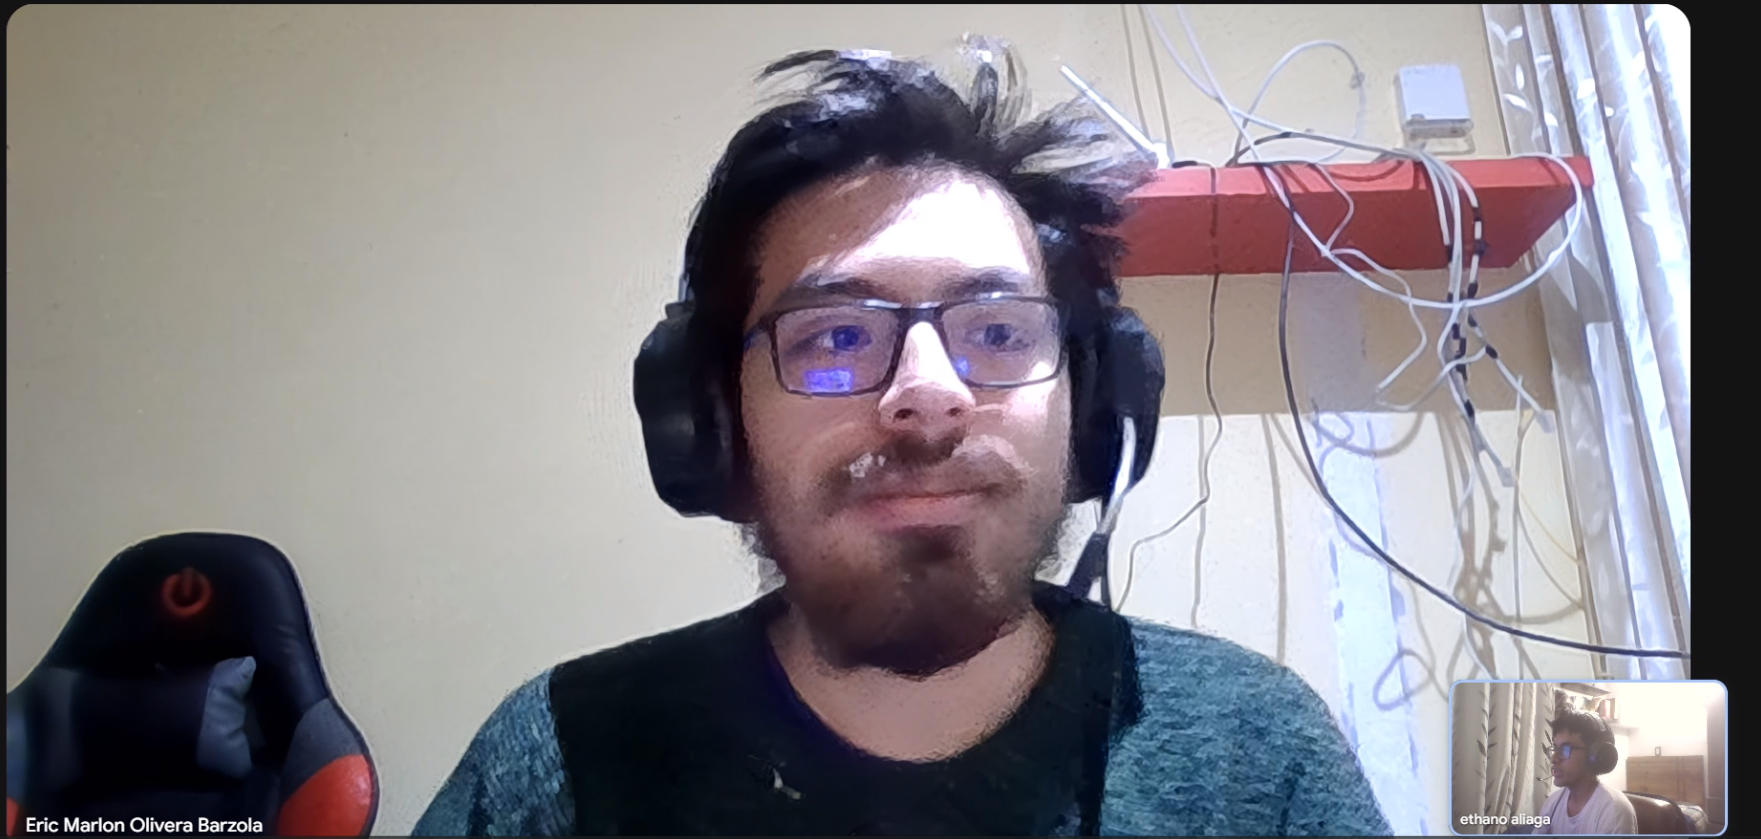
\includegraphics[keepaspectratio,alt={Entrevista Eric}]{assets/img/cap2/entrevista-3.png}}
\caption{Entrevista Eric}
\end{figure}

\textbf{Resumen de la entrevista:}

\begin{itemize}
\tightlist
\item
  \textbf{Contexto y métodos actuales:} Utiliza herramientas digitales
  como Duolingo, además de consumir contenido en inglés (series y
  películas con subtítulos). Ocasionalmente practica con amigos
  cercanos, pero no asiste a clases formales actualmente.
\item
  \textbf{Principales limitaciones:} Presenta dificultades relacionadas
  con la falta de constancia debido a responsabilidades académicas y la
  dificultad para encontrar personas con quienes practicar en tiempo
  real. Además, experimenta vergüenza y miedo a equivocarse,
  especialmente al interactuar con desconocidos o al no contar con
  suficiente vocabulario.
\item
  \textbf{Preferencias de entorno y lugares:} Prefiere entornos
  académicos y estructurados, donde se sienta más cómodo y seguro. En
  cuanto a espacios físicos, opta por cafeterías, ya que las percibe
  como lugares tranquilos y adecuados para mantener conversaciones sin
  interrupciones.
\item
  \textbf{Motivaciones y perfil de compañeros:} Su principal motivación
  es el \textbf{desarrollo profesional}, reconociendo el inglés como una
  herramienta clave para acceder a mejores oportunidades laborales. Está
  dispuesto a asistir con una frecuencia de 1 a 2 veces por semana,
  dependiendo de su disponibilidad. Prefiere iniciar con personas de su
  mismo nivel, aunque también considera valioso interactuar con
  hablantes más avanzados progresivamente.
\item
  \textbf{Rol en conversaciones:} Tiende a adoptar un rol más
  \textbf{reservado al inicio}, participando poco mientras gana
  confianza. Con el tiempo, se vuelve más activo y participativo en la
  conversación.
\item
  \textbf{Expectativas e inquietudes sobre la aplicación:} Espera que la
  plataforma sea \textbf{fácil de usar} y permita visualizar el nivel de
  los participantes para formar grupos equilibrados. Los factores clave
  para generar confianza son la \textbf{verificación de perfiles}, la
  existencia de \textbf{reseñas} y la presencia de \textbf{moderadores o
  facilitadores}. Además, valora que las dinámicas eviten situaciones
  donde algunos participantes dominen la conversación y limiten la
  participación de otros.
\end{itemize}

\paragraph{Segmento 2: Administradores que ofrecen su establecimiento
como punto de
reunión}\label{report__20-cap2-requirements-analysis.md__segmento-2-administradores-que-ofrecen-su-establecimiento-como-punto-de-reuniuxf3n}

\textbf{Entrevista N°1: Virgilio Sanchez}

\begin{itemize}
\tightlist
\item
  Sexo: Masculino
\item
  Edad: 65 años
\item
  Link:
  \url{https://upcedupe-my.sharepoint.com/:v:/g/personal/u202318323_upc_edu_pe/IQBEM5B_aIDCSLpXh7So9i2xAZHFPevkYbwJ9FiRhPvnYc4?e=3lSEOG&nav=eyJyZWZlcnJhbEluZm8iOnsicmVmZXJyYWxBcHAiOiJTdHJlYW1XZWJBcHAiLCJyZWZlcnJhbFZpZXciOiJTaGFyZURpYWxvZy1MaW5rIiwicmVmZXJyYWxBcHBQbGF0Zm9ybSI6IldlYiIsInJlZmVycmFsTW9kZSI6InZpZXcifX0\%3D}
\item
  Inicia en: 0:36
\item
  Duración: 5:56
\end{itemize}

\begin{figure}
\centering
\pandocbounded{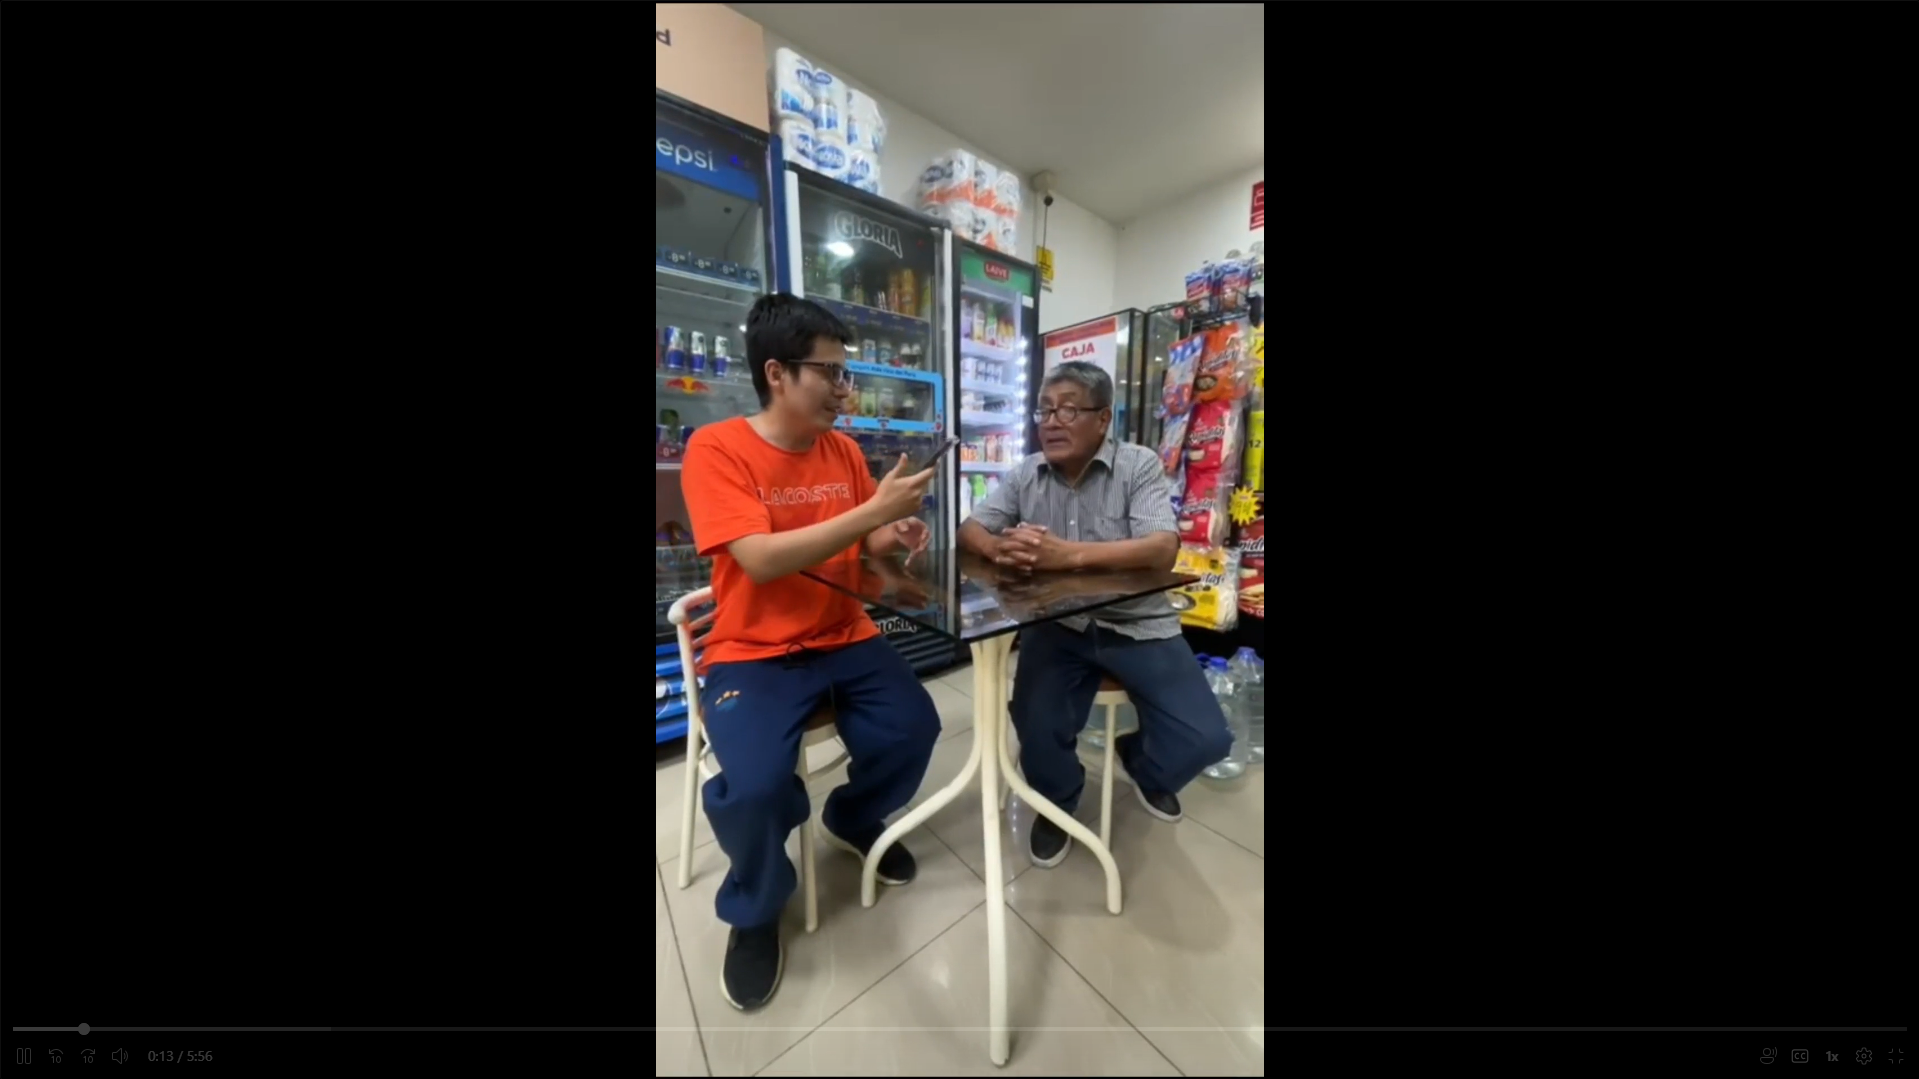
\includegraphics[keepaspectratio,alt={Entrevista Virgilio}]{assets/img/cap2/entrevista-2-1.png}}
\caption{Entrevista Virgilio}
\end{figure}

\textbf{Resumen de la entrevista:}

\begin{itemize}
\tightlist
\item
  \textbf{Contexto del establecimiento:} Administra una
  panadería/cafetería muy cercana a una universidad. Su horario punta es
  por las mañanas (7 a 9 AM) y el negocio familiar cuenta con un total
  de 4 sucursales en el distrito.
\item
  \textbf{Gestión de grupos y reservas:} Actualmente no manejan reservas
  de mesas. Tuvieron malas experiencias pasadas con pedidos muy grandes
  que no fueron pagados, por lo que es vital un sistema de compromiso
  seguro.
\item
  \textbf{Disposición como punto de encuentro:} Está totalmente
  dispuesto y le parece una gran idea. Comenta que los universitarios ya
  frecuentan el local para hacer trabajos o estudiar, por lo que el
  ambiente casual se adapta perfectamente a reuniones para practicar
  idiomas, sin imponer condiciones restrictivas.
\item
  \textbf{Expectativa de consumo:} Espera que, mientras conversan, los
  estudiantes soliciten productos de la vitrina como bocaditos
  (empanadas, alfajores, pasteles, trozos de pizza) y bebidas (café o
  gaseosas).
\item
  \textbf{Expectativas estructurales de la app:} Espera que la
  aplicación funcione como una herramienta de visibilidad, indicando su
  ubicación exacta, cómo llegar y su catálogo de productos para atraer
  más consumidores a sus locales.
\item
  \textbf{Manejo de promociones e incentivos:} Está abierto a brindar
  descuentos y armar combos especiales (ej. empanada + gaseosa) para los
  usuarios de la plataforma, reconociendo que son un imán de clientes.
  Sin embargo, enfatiza que él y sus socios prefieren \textbf{definir
  sus propias promociones}, en lugar de que la aplicación las genere
  automáticamente.
\end{itemize}

\textbf{Entrevista N°1: Yamilie Francia}

\begin{itemize}
\tightlist
\item
  Sexo: Femenimo
\item
  Edad: 26 años
\item
  Link: \url{https://www.youtube.com/watch?v=Y0F_L92XEGc}
\item
  Inicia en: 0:06
\item
  Duración: 5:49
\end{itemize}

\begin{figure}
\centering
\pandocbounded{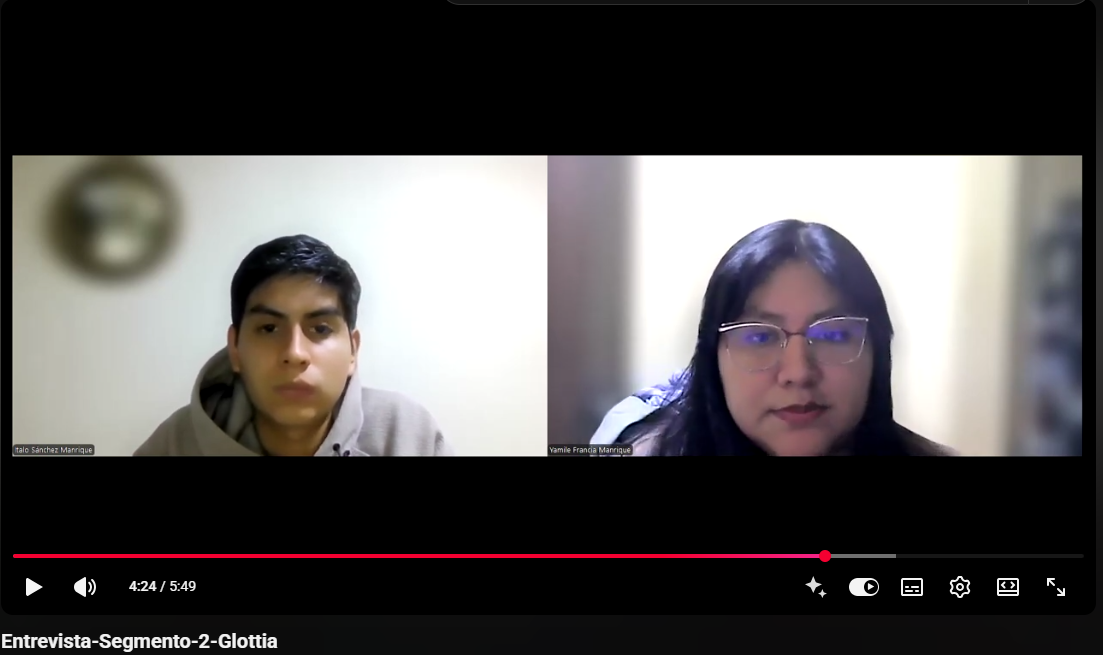
\includegraphics[keepaspectratio,alt={Entrevista Yamile}]{assets/img/cap2/entrevista-Yamile.png}}
\caption{Entrevista Yamile}
\end{figure}

\textbf{Resumen de la entrevista:}

\begin{itemize}
\item
  \textbf{Contexto del establecimiento:} Administra la cafetería ``21
  Grados'' en Carmen de la Legua. Sus horarios de mayor afluencia son de
  8:00 a.m. a 11:00 a.m. y por la noche, mientras que presenta horas de
  baja demanda entre las 2:00 p.m. y las 5:00 p.m., lo que representa
  una oportunidad para atraer nuevos clientes.
\item
  \textbf{Gestión de grupos y reservas:} Actualmente gestiona reservas
  de manera informal a través de WhatsApp y redes sociales,
  registrándolas manualmente en cuadernos. Ha tenido problemas con
  cancelaciones sin previo aviso, lo que genera pérdidas y
  desorganización, por lo que considera necesario un sistema más
  confiable.
\item
  \textbf{Disposición como punto de encuentro:} Está totalmente
  dispuesta a ofrecer su cafetería como espacio para encuentros.
  Considera que el ambiente es ideal para este tipo de actividades y que
  puede atraer a un público joven y dinámico, siempre que no afecte a
  sus clientes habituales.
\item
  \textbf{Expectativa de consumo:} Espera como mínimo el consumo de una
  bebida por asistente, aunque considera ideal incentivar la compra de
  alimentos o combos grupales para aumentar el ticket promedio.
\item
  \textbf{Expectativas estructurales de la app:} Espera que la
  aplicación permita gestionar reservas de forma clara, controlar aforo,
  reducir inasistencias mediante confirmaciones seguras y optimizar la
  organización del negocio, especialmente en horarios de baja demanda.
\item
  \textbf{Manejo de promociones e incentivos:} Está dispuesta a ofrecer
  descuentos, combos grupales y promociones por horario para atraer
  clientes. Sin embargo, enfatiza que prefiere \textbf{tener control
  total sobre sus propias promociones}, aunque valora recibir
  sugerencias basadas en datos y comportamiento de los usuarios.
\end{itemize}

\subsubsection{2.2.3 Análisis de
entrevistas}\label{report__20-cap2-requirements-analysis.md__anuxe1lisis-de-entrevistas}

En este apartado se realiza un análisis de las entrevistas realizadas a
los segmentos objetivo, identificando patrones, insights y oportunidades
clave para el diseño de la solución.

\paragraph{Segmento 1: Usuarios aprendices de idiomas (Análisis
Estadístico)}\label{report__20-cap2-requirements-analysis.md__segmento-1-usuarios-aprendices-de-idiomas-anuxe1lisis-estaduxedstico}

Total de entrevistas: 3

A partir de las entrevistas realizadas a los usuarios del Segmento 1
(jóvenes universitarios aprendices de idiomas), se han extraído métricas
contundentes sobre sus percepciones, hábitos y dolores. A continuación,
se presenta el análisis estadístico respaldado visualmente:

\textbf{1. Principales obstáculos en el aprendizaje}

\begin{figure}
\centering
\pandocbounded{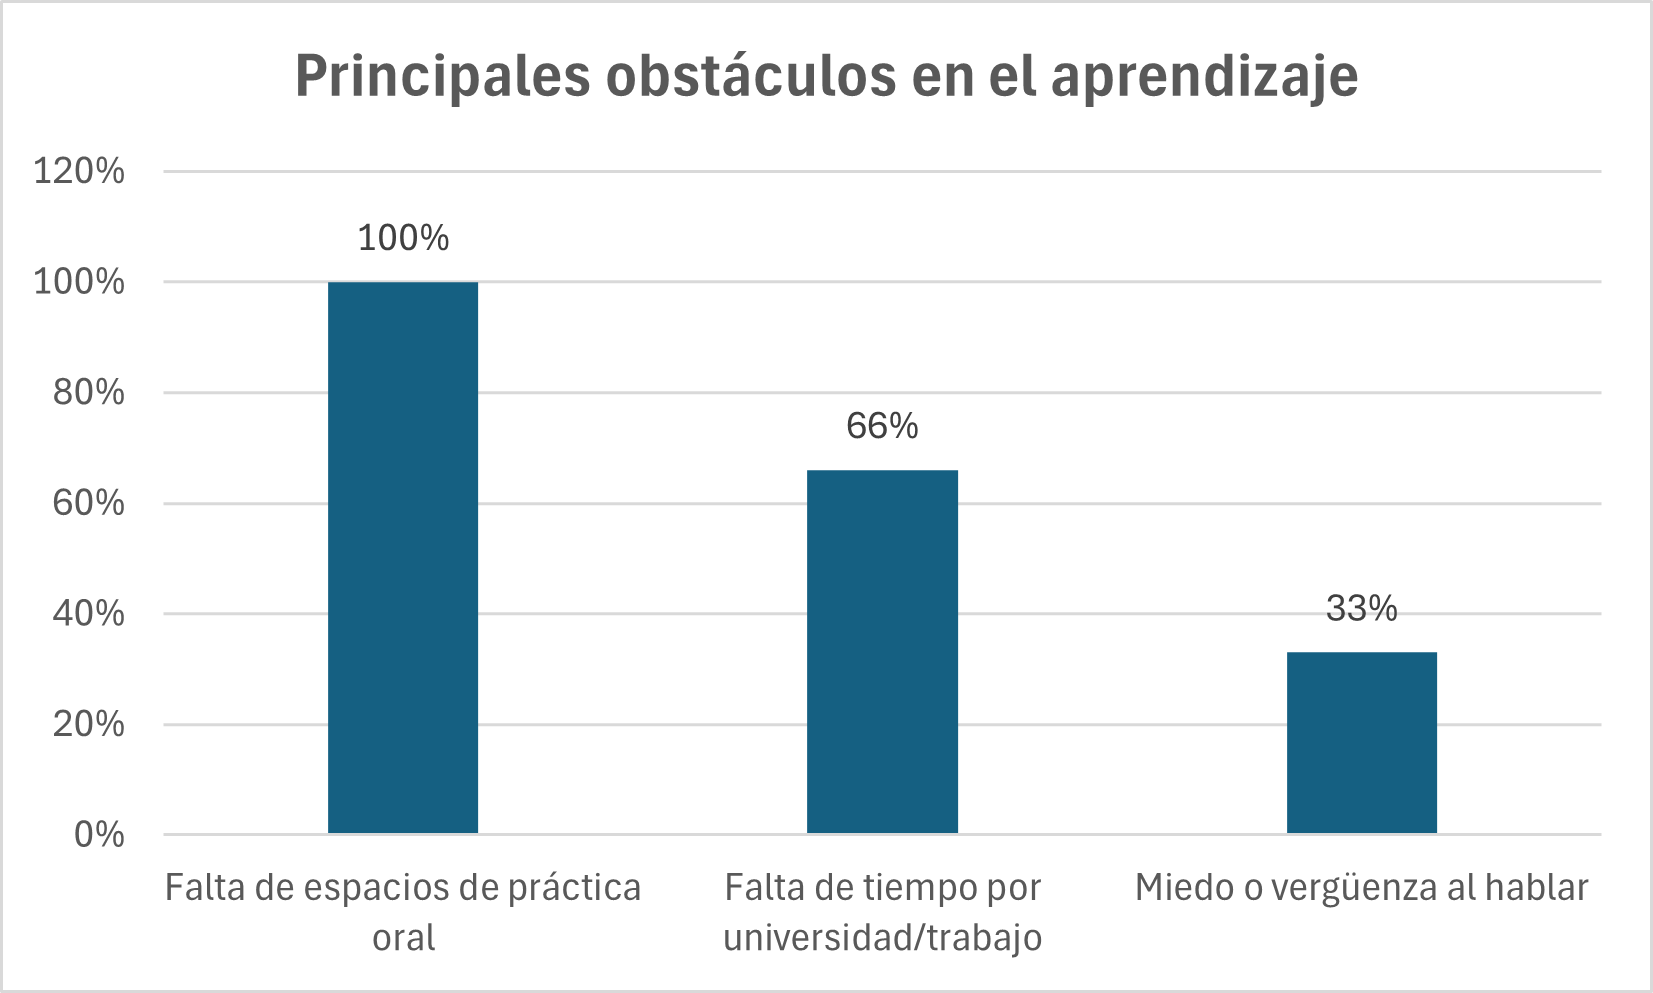
\includegraphics[keepaspectratio,alt={Principales obstáculos en el aprendizaje}]{assets/img/cap2/analisis-entrevista-1.png}}
\caption{Principales obstáculos en el aprendizaje}
\end{figure}

\textbf{Conclusión:} La \emph{falta de espacios para práctica oral}
representa una barrera absoluta (100\%) para los entrevistados. Sumado a
la falta de tiempo (66\%) y la inseguridad (33\%), esto corrobora la
premisa de Glottia: existe una necesidad urgente de proveer entornos
físicos accesibles, cercanos y amigables estructurados exclusivamente
para la expresión oral.

\textbf{2. Preferencias de nivel del compañero de conversación}

\begin{figure}
\centering
\pandocbounded{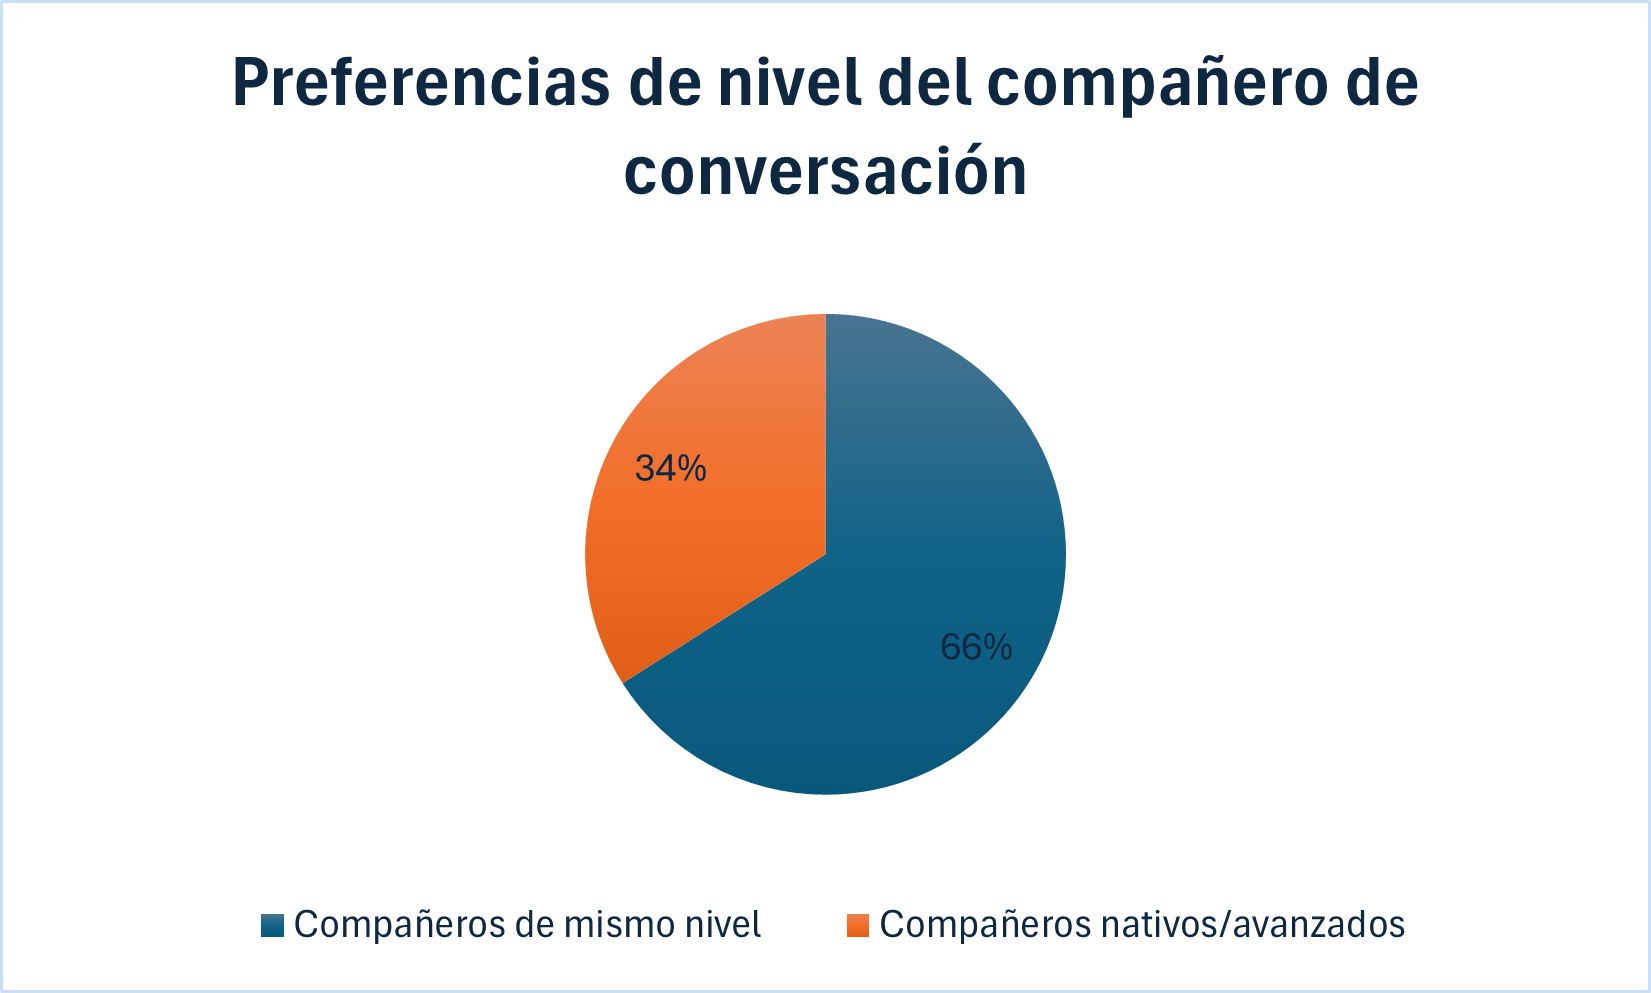
\includegraphics[keepaspectratio,alt={Preferencias de nivel del compañero de conversación}]{assets/img/cap2/analisis-entrevista-2.png}}
\caption{Preferencias de nivel del compañero de conversación}
\end{figure}

\textbf{Conclusión:} El 66\% de los usuarios prefiere conversar con
pares de su mismo nivel para generar mayor confianza y disminuir la
presión al hablar (temor a ser juzgados), mientras que el 34\% prefiere
interactuar con nativos o usuarios nivel avanzado. Esto evidencia que el
sistema de búsqueda o match de Glottia debe tener como prioridad el
filtro por niveles de fluidez.

\textbf{3. Factores de confianza exigidos a la plataforma}

\begin{figure}
\centering
\pandocbounded{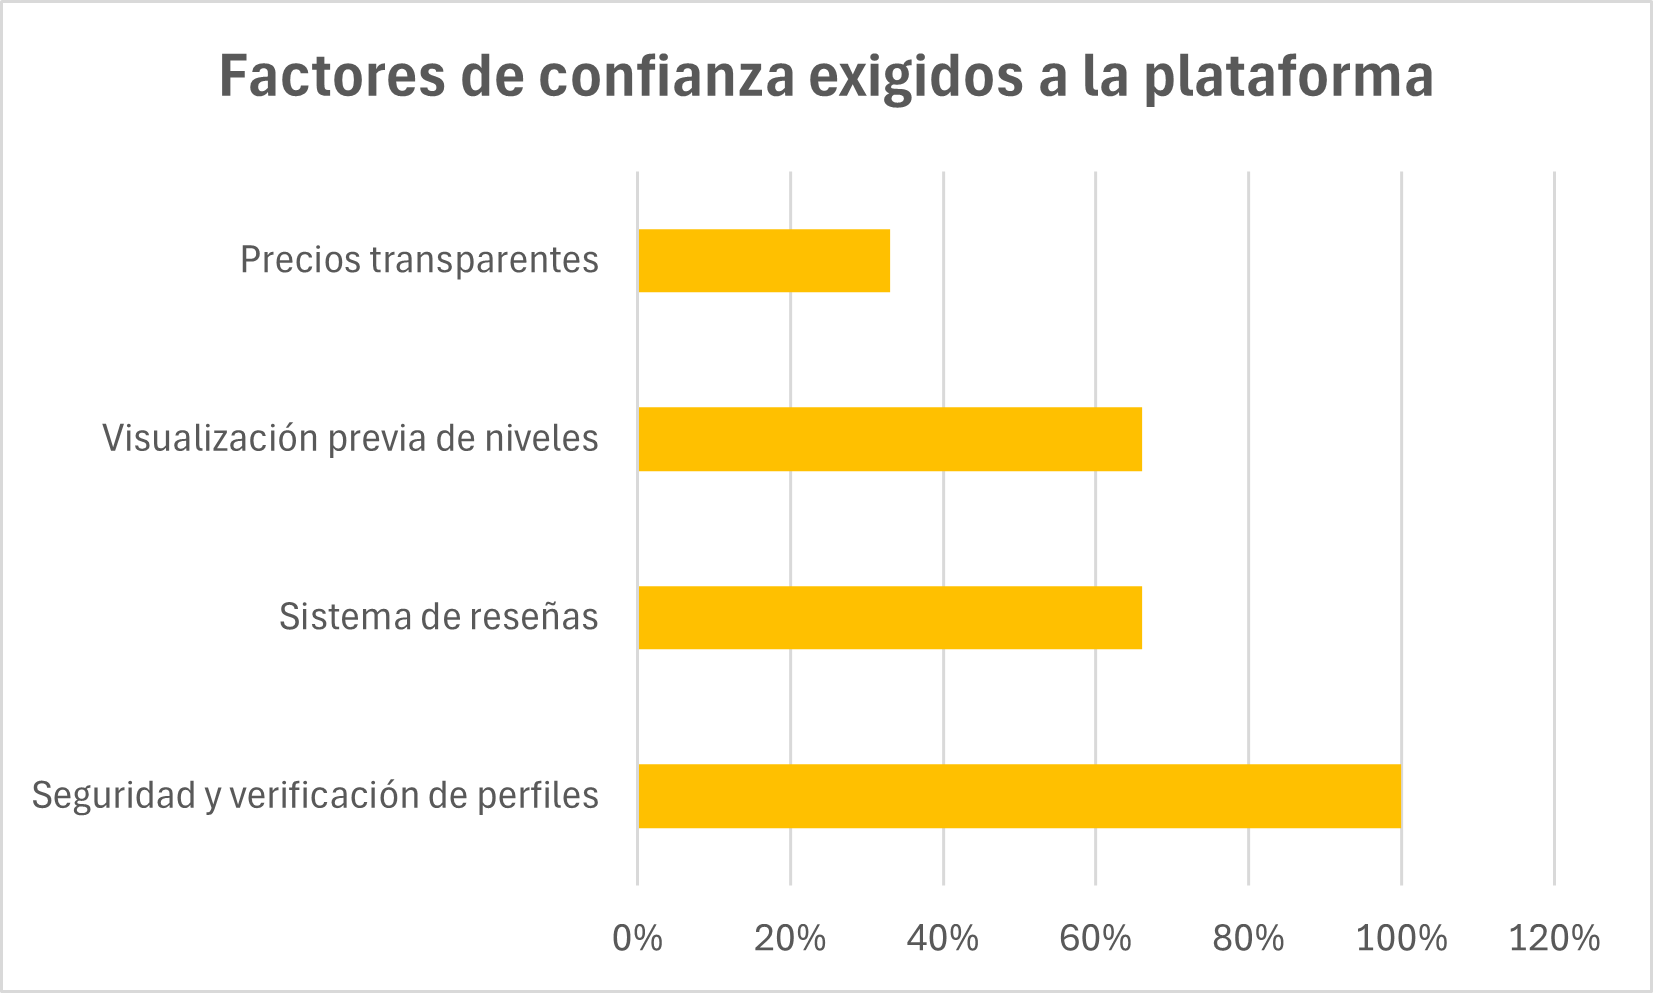
\includegraphics[keepaspectratio,alt={Factores de confianza exigidos a la plataforma}]{assets/img/cap2/analisis-entrevista-3.png}}
\caption{Factores de confianza exigidos a la plataforma}
\end{figure}

\textbf{Conclusión:} Para atreverse a llevar la aplicación al plano
presencial (reunirse), el requerimiento máximo (100\%) es la
\emph{seguridad y verificación de perfiles}. Características como un
sistema de reseñas y ver el nivel del compañero representan un factor
importante para el 66\% de la muestra. Esto indica arquitectónicamente
que el \emph{Core} inicial del diseño de software debe integrar fuertes
validaciones de identidad (Identity Management).

\textbf{4. Opinión y Nivel de Acuerdo con la Aplicación Glottia}

\begin{figure}
\centering
\pandocbounded{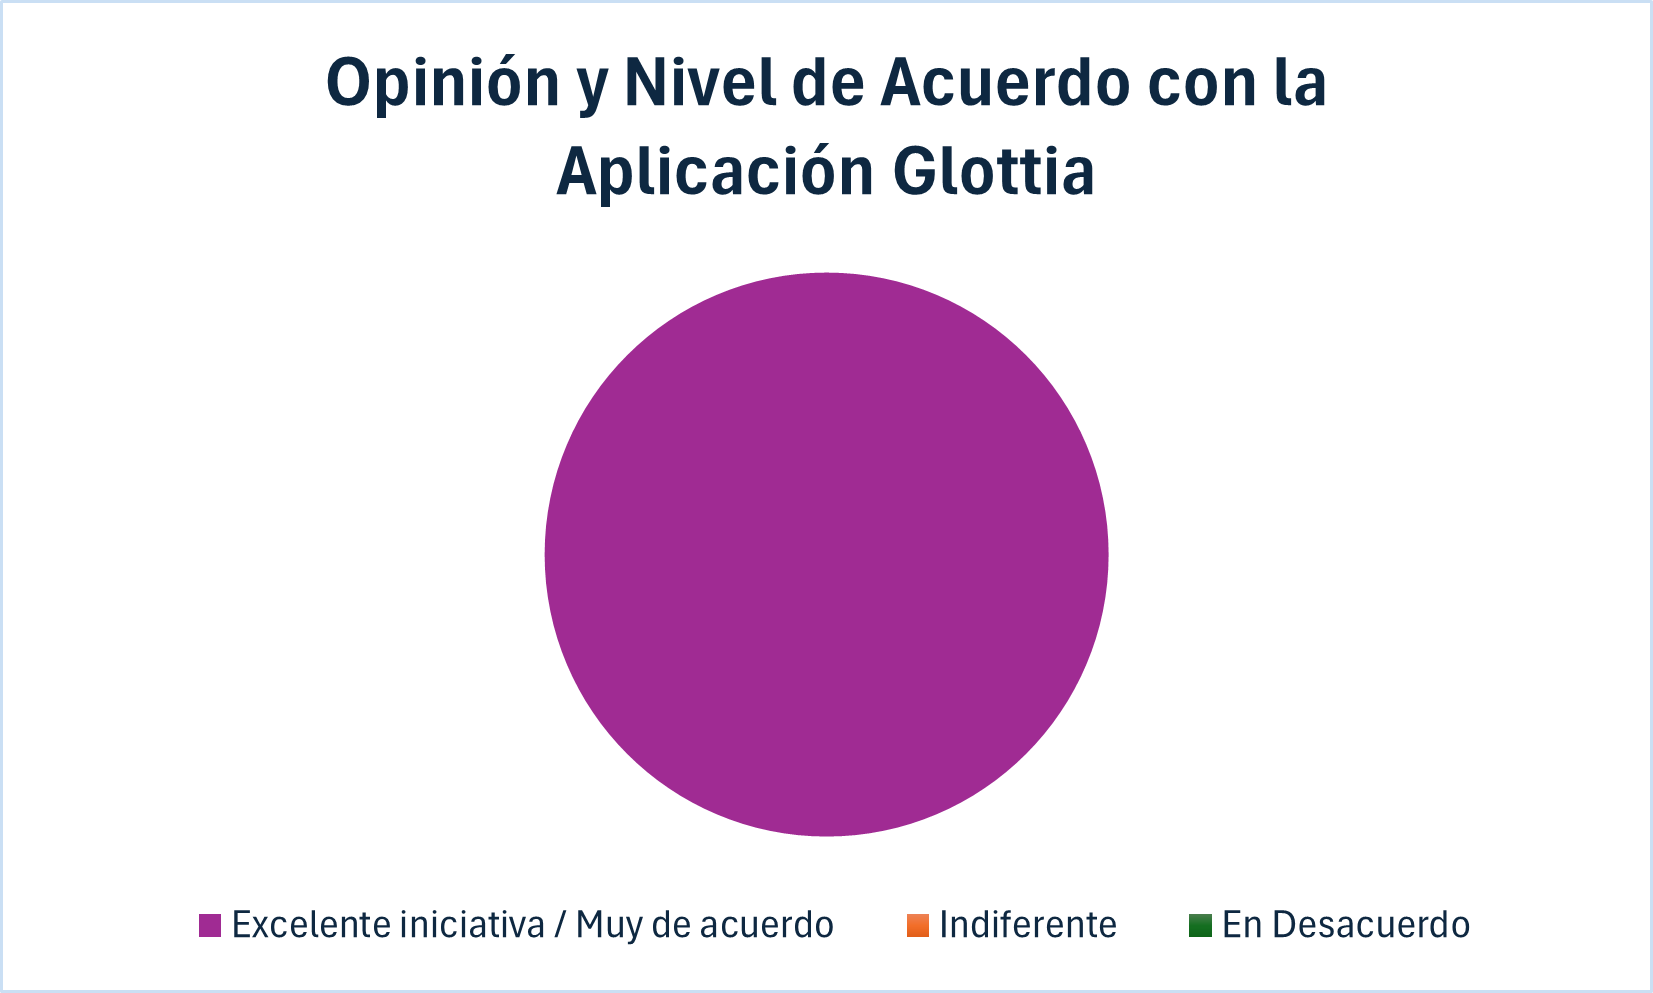
\includegraphics[keepaspectratio,alt={Opinión y Nivel de Acuerdo con la Aplicación Glottia}]{assets/img/cap2/analisis-entrevista-4.png}}
\caption{Opinión y Nivel de Acuerdo con la Aplicación Glottia}
\end{figure}

\textbf{Conclusión:} Existe una total validación del concepto. El 100\%
de la muestra lo consideró una excelente iniciativa y declaró estar
completamente de acuerdo en que la plataforma aliviaría sus mayores
frustraciones cotidianas de aprendizaje, lo cual avala contundentemente
la viabilidad del mercado y la deseabilidad del producto.

\paragraph{Segmento 2: Administradores que ofrecen su establecimiento
como punto de
reunión}\label{report__20-cap2-requirements-analysis.md__segmento-2-administradores-que-ofrecen-su-establecimiento-como-punto-de-reuniuxf3n-1}

Total de entrevistas: 3

A partir de las entrevistas realizadas a los administradores de
establecimientos, se han extraído métricas clave sobre su disposición,
expectativas y condiciones para colaborar con una plataforma como
Glottia. A continuación, se presenta el análisis estadístico respaldado
visualmente:

\textbf{1. Disposición a ofrecer su establecimiento como punto de
encuentro}

\begin{figure}
\centering
\pandocbounded{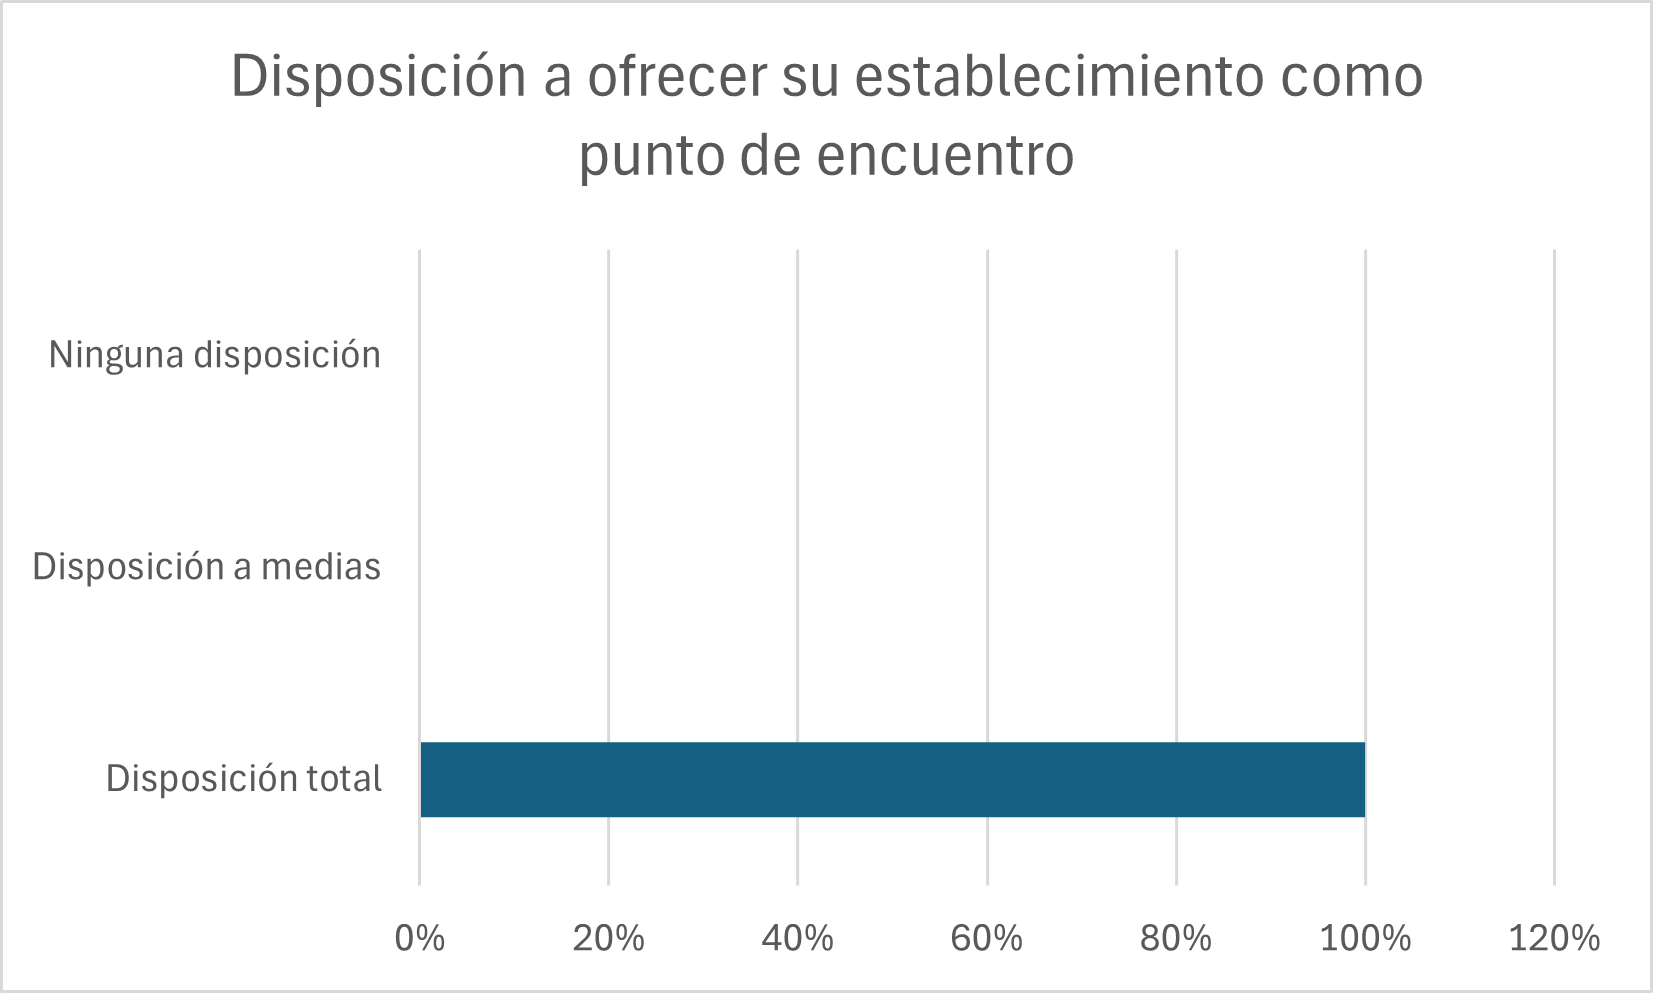
\includegraphics[keepaspectratio,alt={Disposición a ofrecer su establecimiento como punto de encuentro}]{assets/img/cap2/analisis-entrevista-5.png}}
\caption{Disposición a ofrecer su establecimiento como punto de
encuentro}
\end{figure}

\textbf{Conclusión:} El 100\% de los administradores muestra una
disposición total para afiliarse a Glottia y prestar sus locales. Ven en
la plataforma una iniciativa altamente viable que les permite atraer a
un público joven y utilizar productivamente sus ``horas muertas'',
confirmando la deseabilidad del modelo de negocio desde la perspectiva
de la oferta (Supply-side).

\textbf{2. Expectativas de consumo durante los encuentros}

\begin{figure}
\centering
\pandocbounded{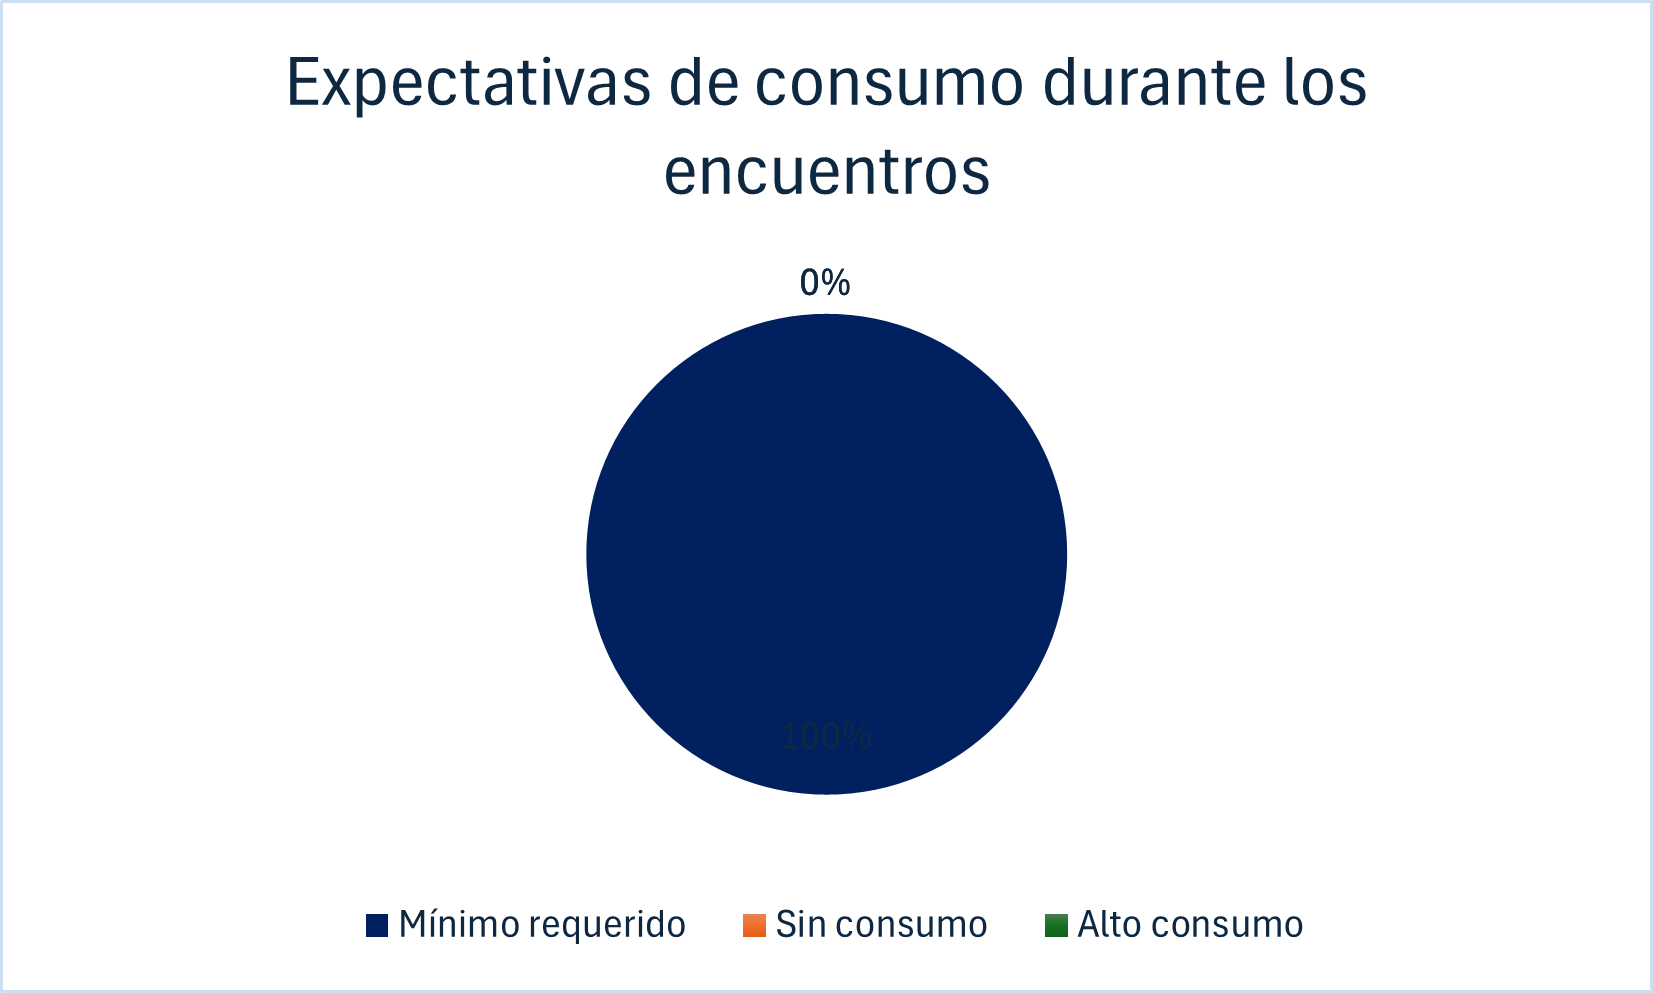
\includegraphics[keepaspectratio,alt={Expectativas de consumo durante los encuentros}]{assets/img/cap2/analisis-entrevista-6.png}}
\caption{Expectativas de consumo durante los encuentros}
\end{figure}

\textbf{Conclusión:} Existe un consenso (100\%) en exigir un consumo
mínimo garantizado (al menos una bebida por asistente) para justificar
la ocupación de las mesas, con un especial interés en lograr la venta de
alimentos o ``combos grupales''. Esto indica que Glottia debe establecer
políticas claras de consumo mínimo dentro de los términos y condiciones
de las reservas generadas desde la app.

\textbf{3. Preferencia en la gestión de promociones e incentivos}

\begin{figure}
\centering
\pandocbounded{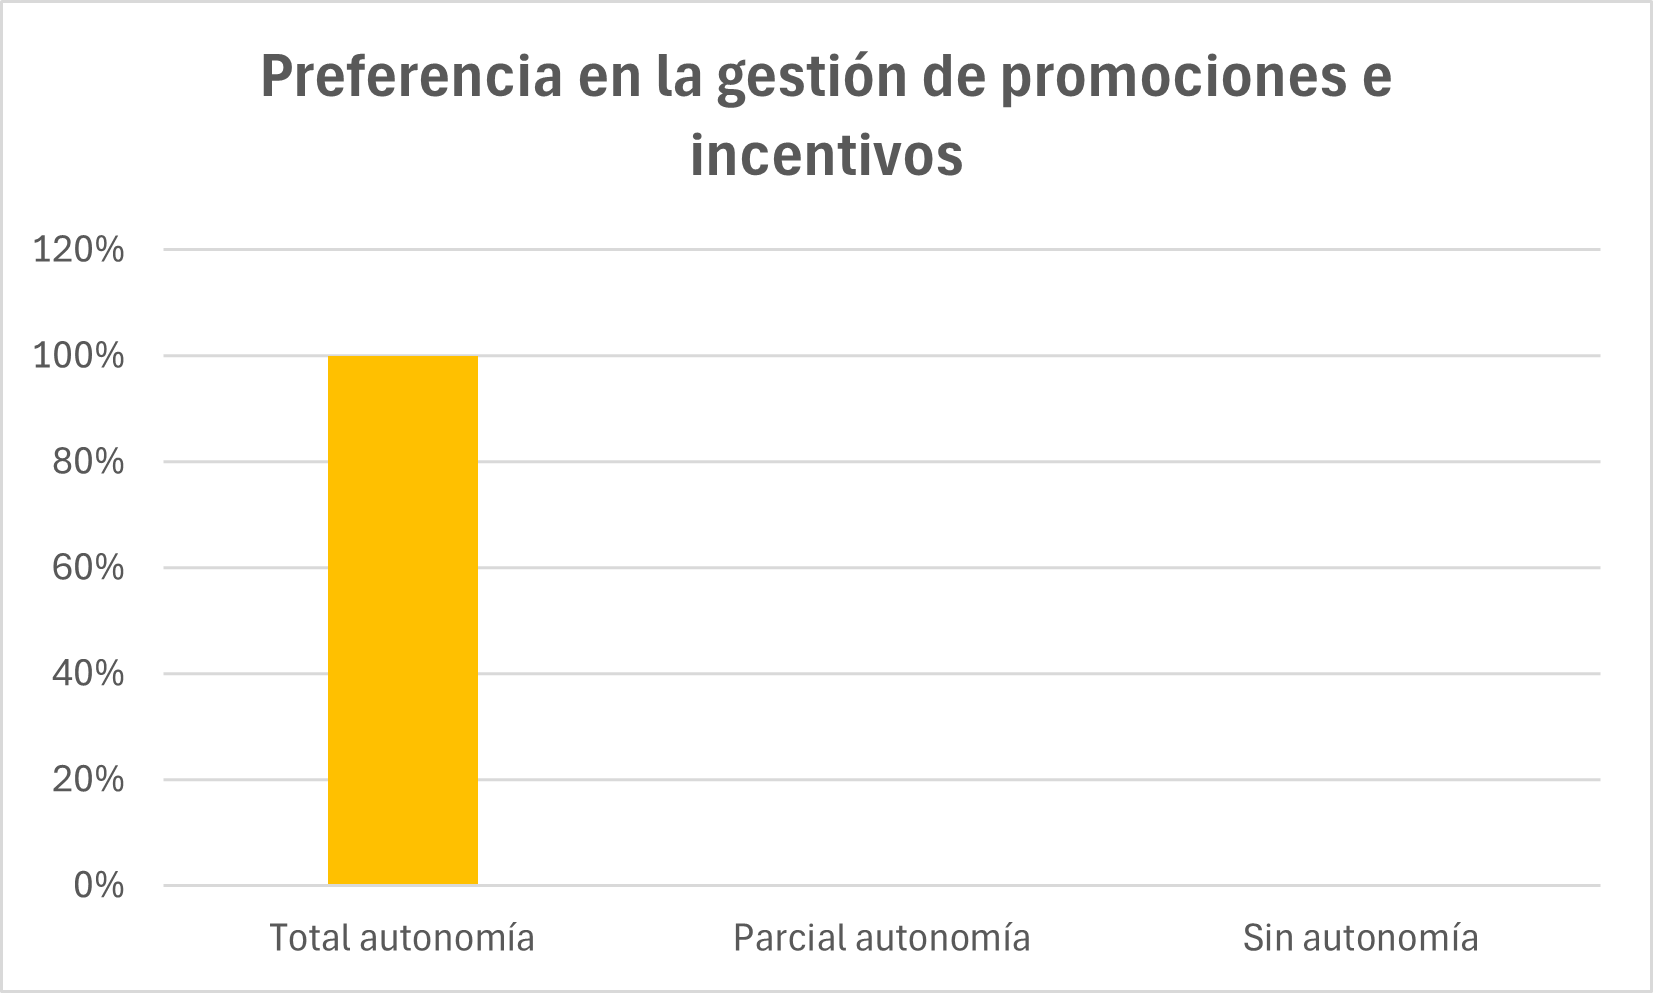
\includegraphics[keepaspectratio,alt={Preferencia en la gestión de promociones e incentivos}]{assets/img/cap2/analisis-entrevista-7.png}}
\caption{Preferencia en la gestión de promociones e incentivos}
\end{figure}

\textbf{Conclusión:} La totalidad de los entrevistados (100\%) requiere
tener autonomía absoluta para definir, configurar y activar sus propias
promociones, rechazando que la aplicación genere descuentos automáticos
sin su control. Arquitectónicamente, esto revalida la necesidad
fundamental de desarrollar un \textbf{Panel Gestor (Dashboard B2B)}
donde los aliados manejen directamente todo su inventario y cupones.

\textbf{4. Expectativas estructurales de la aplicación para su negocio}

\begin{figure}
\centering
\pandocbounded{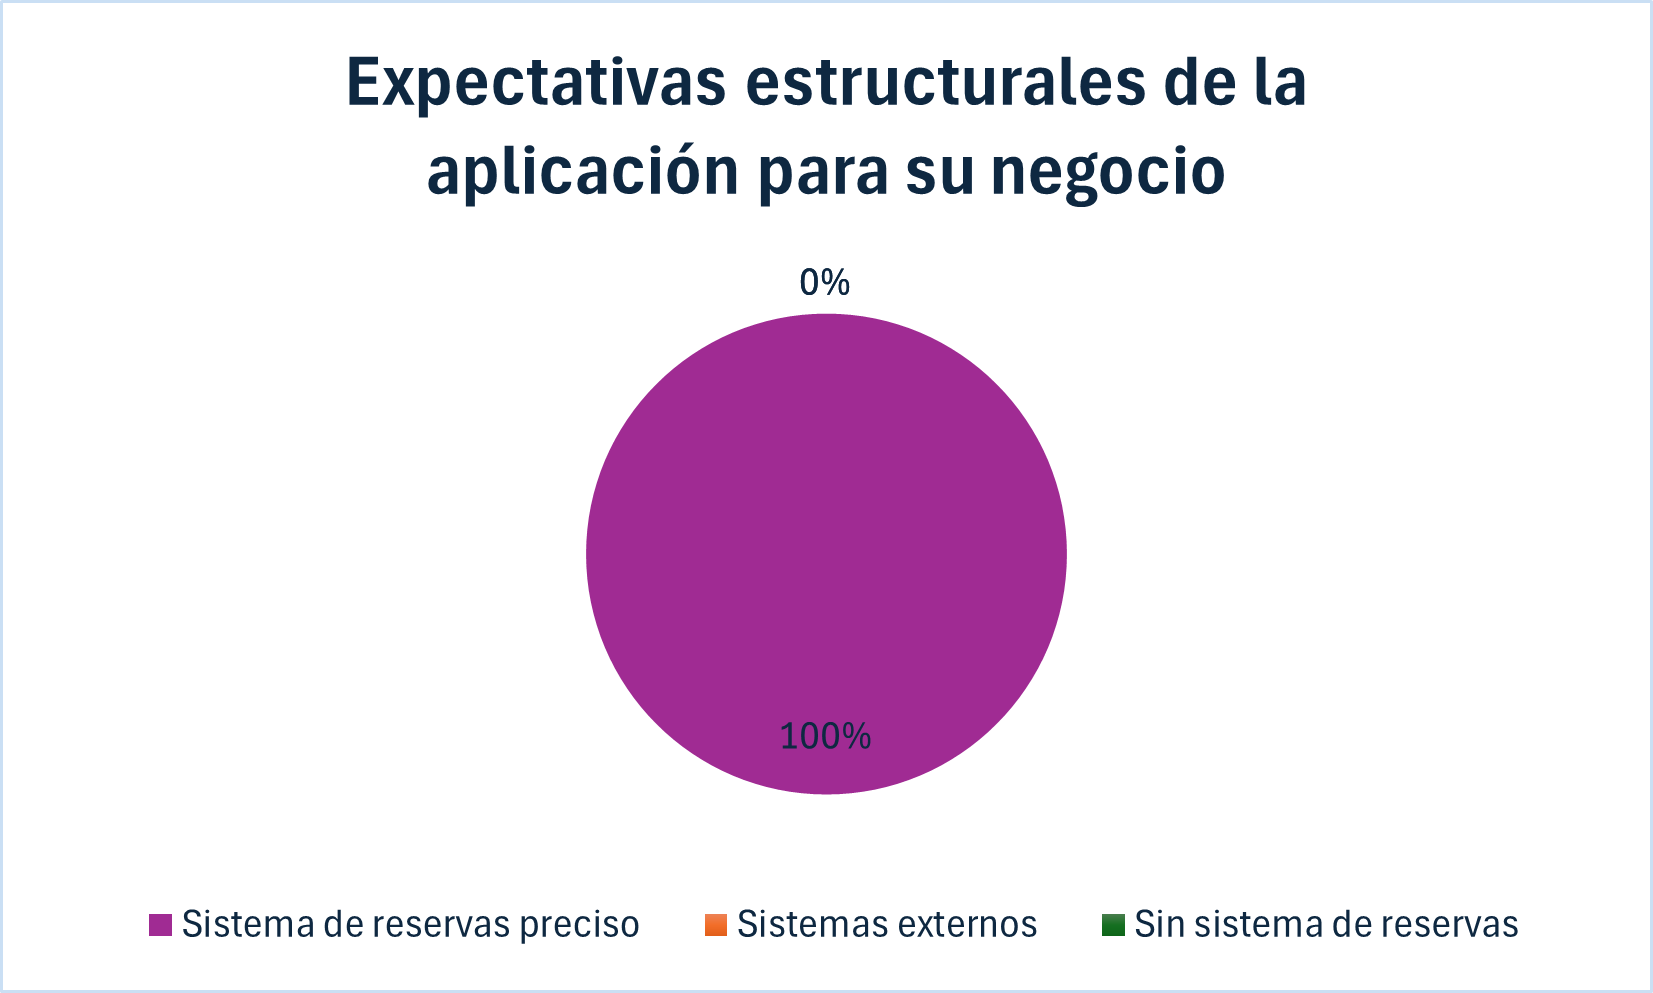
\includegraphics[keepaspectratio,alt={Expectativas estructurales de la aplicación para su negocio}]{assets/img/cap2/analisis-entrevista-8.png}}
\caption{Expectativas estructurales de la aplicación para su negocio}
\end{figure}

\textbf{Conclusión:} Para mitigar su frustración actual relacionada a
anulaciones y mesas bloqueadas innecesariamente, el 100\% exige un
sistema de reservas preciso con control estricto de aforo. Este
requerimiento consolida la validación 100\% digital (ej.
\textbf{Check-in mediante código QR}) como una de las funciones
\emph{Core} indispensables a programar para garantizar el compromiso de
los asistentes.

\subsection{2.3
Needfinding}\label{report__20-cap2-requirements-analysis.md__needfinding}

En esta seccción, el equipo realiza el proceso de búsqueda de
necesidades en un método cualitativo.

\subsubsection{2.3.1 User
Personas}\label{report__20-cap2-requirements-analysis.md__user-personas}

En la presente sección se presentan las fichas de User Persona
elaboradas teniendo en cuenta las entrevistas realizadas y analizadas
previamente y la revisión de soluciones existentes en el mercado. En
cada arquetipo se presentan las características demográficas, de
personalidad, los objetivos, las motivaciones, frustraciones y
preferencias de los usuarios clave de cada segmento. La construcción de
estos User Persona se basa en resultados y análisis obtenidos durante la
investigación previa con el objetivo de tomar decisiones de diseño y
desarrollo adecuadas para resolver los problemas identificados.

\paragraph{Segmento
1:}\label{report__20-cap2-requirements-analysis.md__segmento-1}

\pandocbounded{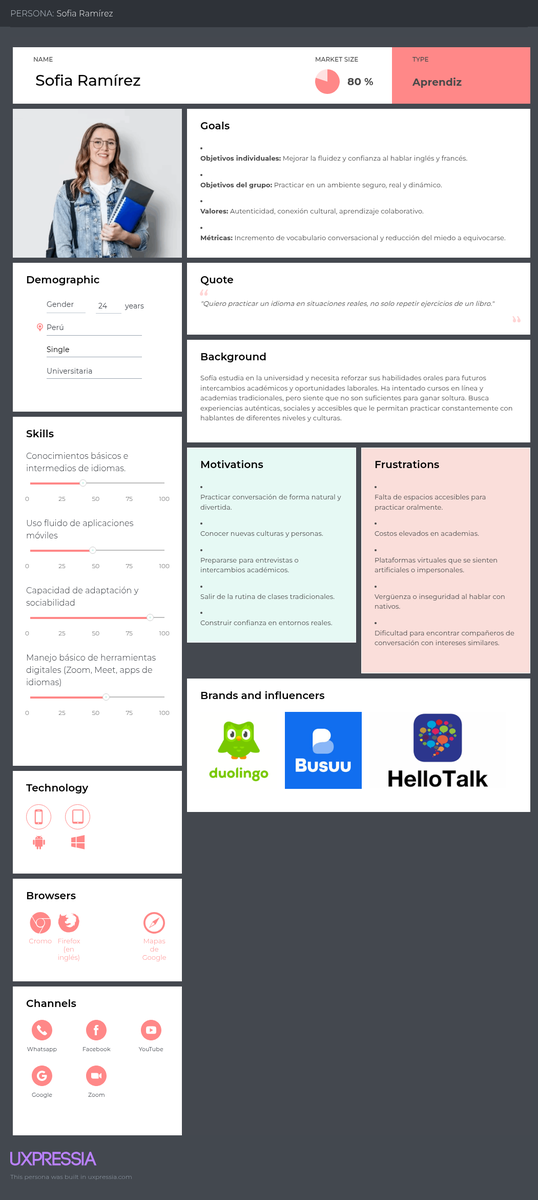
\includegraphics[keepaspectratio]{assets/img/cap2/user-person-1.png}}

\paragraph{Segmento
2:}\label{report__20-cap2-requirements-analysis.md__segmento-2}

\pandocbounded{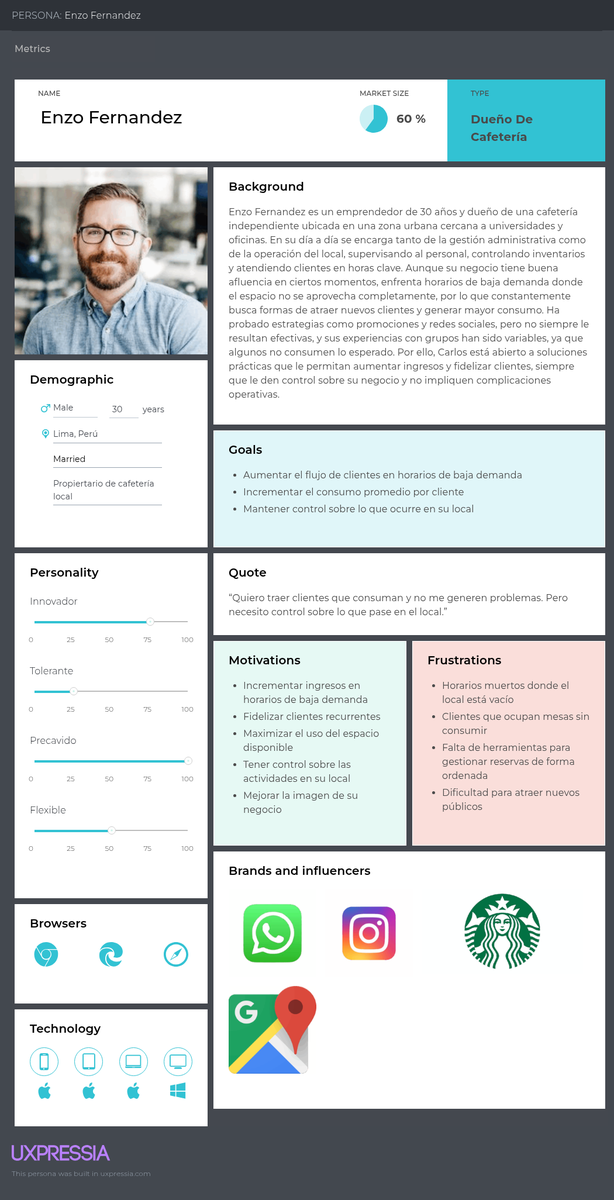
\includegraphics[keepaspectratio]{assets/img/cap2/user-person-2.png}}

\subsubsection{2.3.2 User Task
Matrix}\label{report__20-cap2-requirements-analysis.md__user-task-matrix}

A continuación, se presenta el User Task Matrix alineada a los User
Personas identificados: \textbf{Sofía Ramírez} (Aprendiz Universitaria
que busca fluidez y comunidad) y \textbf{Enzo Fernandez} (Dueño de
Cafetería que busca maximizar sus horas muertas con control y
rentabilidad).

Esta matriz categoriza las acciones principales según la etapa de
interacción de cada usuario con la plataforma Glottia, valorando la
frecuencia con que interactúan y la criticidad de la funcionalidad.

\begin{longtable}{p{4cm} p{3cm} p{2cm} p{2cm} p{2cm}}
\toprule
Etapa / Tarea Principal & Aprendiz (Sofía) & Admin. Local (Enzo) & Frecuencia & Importancia \\
\midrule

\textbf{Onboarding \& Configuración} & & & & \\
Registrar cuenta e iniciar sesión en Glottia & Sí & Sí & Única vez & Alta \\
Completar perfil personal. (idiomas, nivel, gustos) & Sí & No & Única vez & Alta \\
Configurar perfil del local. (fotos, ubicación, políticas) & No & Sí & Única vez & Alta \\
Definir horarios de disponibilidad. & No & Sí & Ocasional & Alta \\

\textbf{Descubrimiento \& Reservas} & & & & \\
Explorar y filtrar encuentros. & Sí & No & Frecuente & Alta \\
Reservar cupo en mesa temática. & Sí & No & Frecuente & Alta \\
Gestionar reservas y aforo. & No & Sí & Frecuente & Alta \\

\textbf{Durante el Encuentro} & & & & \\
Mostrar código QR (Check-in). & Sí & No & Frecuente & Alta \\
Validar ingresos (Check-in). & No & Sí & Frecuente & Alta \\
Redimir descuentos. & Sí & No & Frecuente & Alta \\

\textbf{Retención \& Análisis} & & & & \\
Calificar experiencia. & Sí & Sí & Frecuente & Media \\
Revisar progreso. & Sí & No & Frecuente & Alta \\
Visualizar dashboard. & No & Sí & Frecuente & Alta \\
Activar promociones. & No & Sí & Ocasional & Media \\

\bottomrule
\end{longtable}

\emph{(Leyenda: \textbf{Sí} = El segmento realiza la tarea de forma
directa; \textbf{-} = El segmento no realiza o no requiere acceso a esta
tarea)}

\textbf{Análisis del User Task Matrix:}

El desarrollo de esta matriz revela hallazgos clave para la arquitectura
de la solución y la priorización del \emph{Product Backlog} en futuras
iteraciones:

\begin{enumerate}
\def\labelenumi{\arabic{enumi}.}
\tightlist
\item
  \textbf{Intersección Crítica:} El éxito de la plataforma reside en el
  momento de la experiencia híbrida, específicamente en el proceso de
  ``Check-in''. La validación mediante QR es una tarea de frecuencia e
  importancia alta para ambos segmentos, ya que asegura el control de
  aforo y consumo que busca Enzo (Administrador) y garantiza el acceso
  seguro al evento que espera Sofía (Aprendiz).
\item
  \textbf{Estrategias de Retención Diferenciadas:} Las razones por las
  que cada usuario volverá a utilizar la plataforma son totalmente
  distintas. Para mantener motivada a la aprendiz, el sistema debe
  enfocarse en la \textbf{gamificación} (otorgar insignias, mostrar su
  evolución y darle puntos de lealtad) para premiar su constancia. Por
  el contrario, para retener al dueño del local, el sistema debe
  ofrecerle herramientas de \textbf{valor comercial} mediante un panel
  de administración o un dashboard analítico para medir su ROI y la
  opción de activar promociones personalizadas.
\item
  \textbf{Roles Complementarios (Oferta y Demanda):} Se observa una
  clara separación de tareas en la fase de descubrimiento. Sofía tiene
  un rol activo de búsqueda y reserva, mientras que Enzo asume un rol
  asíncrono de configuración de disponibilidad. Esta asimetría indica
  que los flujos de experiencia de usuario serán completamente
  distintos, justificando la creación de interfaces o módulos separados.
\end{enumerate}

\subsubsection{2.3.3 Empathy
Maps}\label{report__20-cap2-requirements-analysis.md__empathy-maps}

\subsubsection{2.3.4 As-is Scenario
Mapping}\label{report__20-cap2-requirements-analysis.md__as-is-scenario-mapping}

\begin{figure}
\centering
\pandocbounded{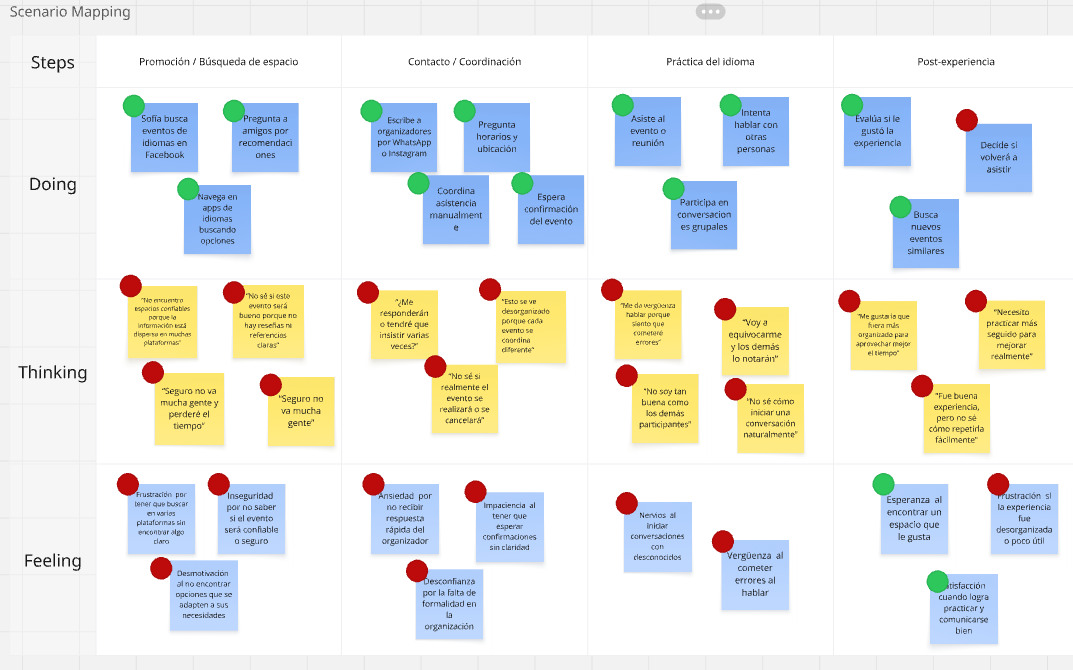
\includegraphics[keepaspectratio,alt={As-Is Segmento 1}]{assets/img/cap2/as-is-scenario-mapping-Sofia.PNG}}
\caption{As-Is Segmento 1}
\end{figure}

\paragraph{Áreas
Negativas}\label{report__20-cap2-requirements-analysis.md__uxe1reas-negativas}

\paragraph{Búsqueda de espacios para practicar
idiomas}\label{report__20-cap2-requirements-analysis.md__buxfasqueda-de-espacios-para-practicar-idiomas}

\begin{itemize}
\tightlist
\item
  Frustración por tener que buscar en múltiples plataformas sin
  encontrar opciones claras.
\item
  Sensación de no encontrar espacios confiables o adecuados a su nivel.
\item
  Incertidumbre por la falta de información sobre eventos (horarios,
  dinámica, asistentes).
\item
  Desmotivación al no encontrar experiencias constantes o accesibles.
\end{itemize}

\begin{center}\rule{0.5\linewidth}{0.5pt}\end{center}

\paragraph{Contacto y
coordinación}\label{report__20-cap2-requirements-analysis.md__contacto-y-coordinaciuxf3n}

\begin{itemize}
\tightlist
\item
  Ansiedad por la falta de respuesta rápida de organizadores.
\item
  Desconfianza debido a la desorganización en la comunicación.
\item
  Incomodidad por tener que usar múltiples aplicaciones para coordinar.
\item
  Inseguridad al no tener confirmación clara del evento o asistencia.
\end{itemize}

\begin{center}\rule{0.5\linewidth}{0.5pt}\end{center}

\paragraph{Práctica del
idioma}\label{report__20-cap2-requirements-analysis.md__pruxe1ctica-del-idioma}

\begin{itemize}
\tightlist
\item
  Vergüenza al hablar con desconocidos por miedo a equivocarse.
\item
  Inseguridad al compararse con personas de mayor nivel.
\item
  Dificultad para iniciar conversaciones en entornos poco estructurados.
\item
  Frustración por no aprovechar al máximo la experiencia de práctica.
\end{itemize}

\begin{center}\rule{0.5\linewidth}{0.5pt}\end{center}

\paragraph{Post-experiencia}\label{report__20-cap2-requirements-analysis.md__post-experiencia}

\begin{itemize}
\tightlist
\item
  Frustración cuando la experiencia fue desorganizada o poco útil.
\item
  Falta de continuidad para seguir practicando regularmente.
\item
  Sensación de que el progreso es lento o inconsistente.
\item
  Dificultad para encontrar nuevamente experiencias similares.
\end{itemize}

\begin{center}\rule{0.5\linewidth}{0.5pt}\end{center}

\paragraph{Áreas
Positivas}\label{report__20-cap2-requirements-analysis.md__uxe1reas-positivas}

\paragraph{Búsqueda de
espacios}\label{report__20-cap2-requirements-analysis.md__buxfasqueda-de-espacios}

\begin{itemize}
\tightlist
\item
  Esperanza al encontrar eventos que parecen interesantes.
\item
  Motivación por aprender idiomas de forma práctica y social.
\item
  Interés en conocer nuevas culturas y personas.
\end{itemize}

\begin{center}\rule{0.5\linewidth}{0.5pt}\end{center}

\paragraph{Contacto y
coordinación}\label{report__20-cap2-requirements-analysis.md__contacto-y-coordinaciuxf3n-1}

\begin{itemize}
\tightlist
\item
  Flexibilidad para adaptarse a diferentes horarios y dinámicas.
\item
  Disposición para interactuar con nuevas personas.
\end{itemize}

\begin{center}\rule{0.5\linewidth}{0.5pt}\end{center}

\paragraph{Práctica del
idioma}\label{report__20-cap2-requirements-analysis.md__pruxe1ctica-del-idioma-1}

\begin{itemize}
\tightlist
\item
  Satisfacción cuando logra comunicarse efectivamente.
\item
  Alegría al conectar con personas de otras culturas.
\item
  Incremento de confianza en momentos de interacción exitosa.
\end{itemize}

\begin{center}\rule{0.5\linewidth}{0.5pt}\end{center}

\paragraph{Post-experiencia}\label{report__20-cap2-requirements-analysis.md__post-experiencia-1}

\begin{itemize}
\tightlist
\item
  Motivación para seguir practicando después de una buena experiencia.
\item
  Esperanza de encontrar espacios más constantes y organizados.
\item
  Interés en repetir experiencias positivas.
\end{itemize}

\begin{center}\rule{0.5\linewidth}{0.5pt}\end{center}

\paragraph{Conclusión}\label{report__20-cap2-requirements-analysis.md__conclusiuxf3n}

Sofía enfrenta múltiples dificultades a lo largo de su proceso de
aprendizaje de idiomas, principalmente en la búsqueda de espacios
adecuados, la coordinación desorganizada y la falta de entornos
estructurados para practicar. Estas limitaciones generan frustración,
inseguridad y poca continuidad en su aprendizaje.

Sin embargo, existen momentos clave de motivación y satisfacción cuando
logra interactuar exitosamente, lo que evidencia un alto interés en este
tipo de experiencias. Esto demuestra la necesidad de una solución como
Glottia, que permita centralizar, organizar y facilitar encuentros
seguros, accesibles y constantes para la práctica de idiomas, mejorando
significativamente la experiencia del usuario.

\section{Capítulo III: Requirements
Specification}\label{report__30-cap3-requirements-spec.md__capuxedtulo-iii-requirements-specification}

En este capítulo se detallan los requisitos del proyecto, incluyendo los
To-be Scenario Mappings, User Stories, Impact Map y el Product Backlog.
Estos elementos son fundamentales para guiar el desarrollo del proyecto
y asegurar que se cumplan las necesidades y expectativas de los usuarios
finales.

\subsection{3.1 To-Be Scenario
Mapping}\label{report__30-cap3-requirements-spec.md__to-be-scenario-mapping}

A continuación se presenta el To-Be Scenario Mapping para la aplicación
de práctica de idiomas, que ilustra cómo los usuarios interactuarán con
el sistema para practicar idiomas en espacios locales. Como tenemos dos
segmentos objetivos (practicantes de idiomas y establecimientos
aliados), se han desarrollado dos escenarios distintos para cada uno de
ellos, con el fin de capturar sus respectivas experiencias y
necesidades.

\subsubsection{Escenario 1: Experiencia del estudiante de
idiomas}\label{report__30-cap3-requirements-spec.md__escenario-1-experiencia-del-estudiante-de-idiomas}

\begin{figure}
\centering
\pandocbounded{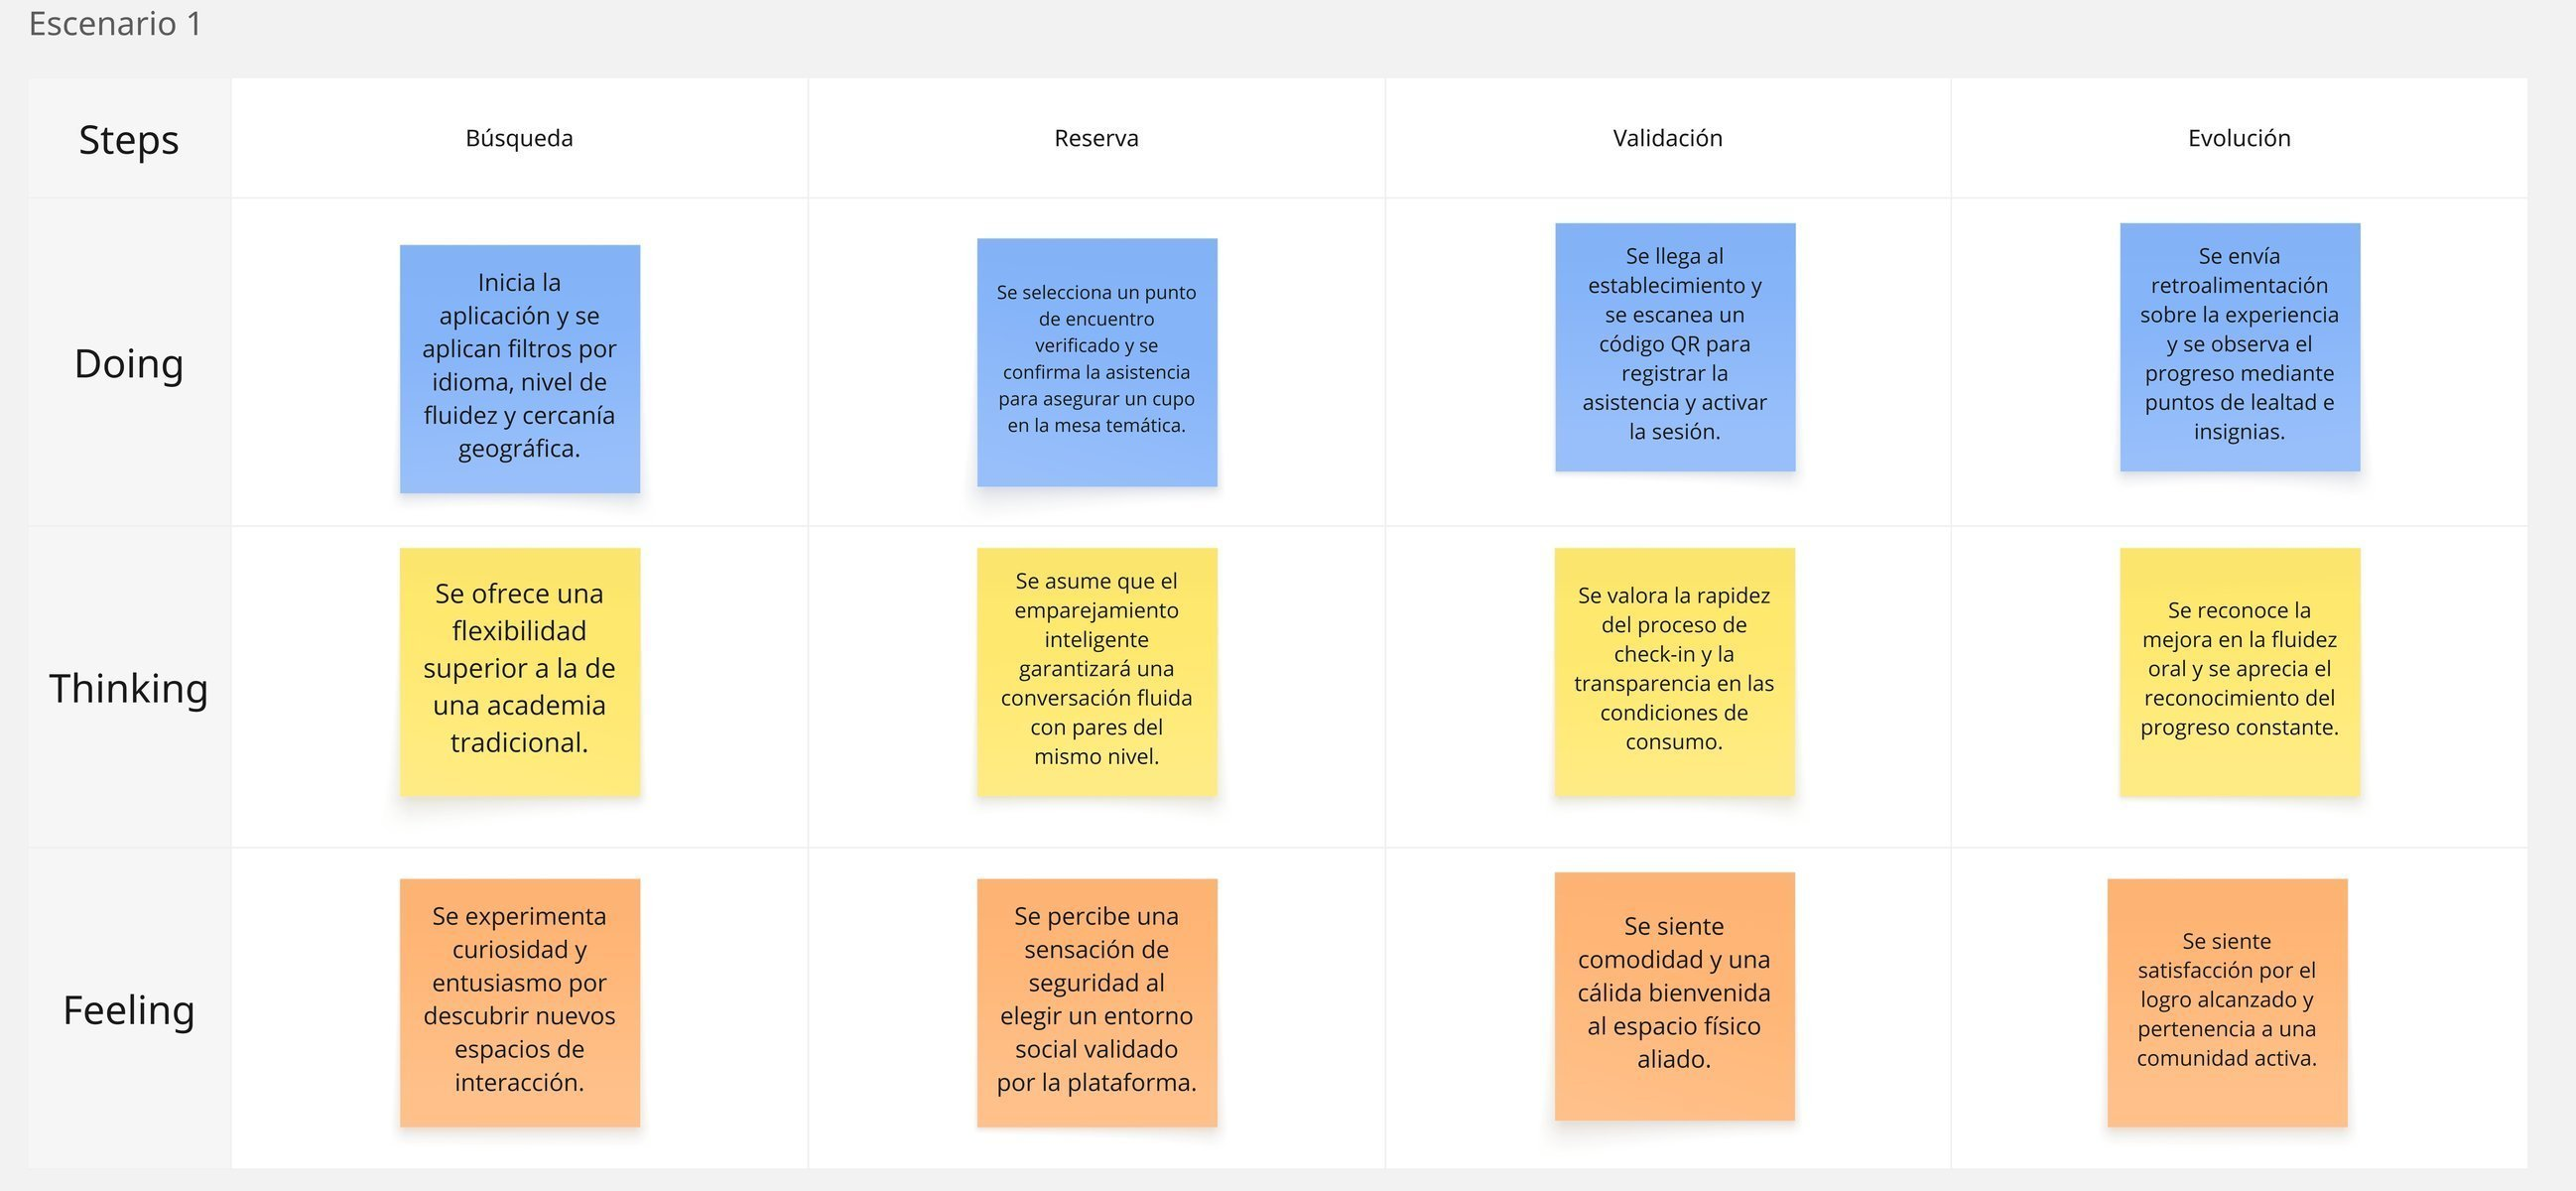
\includegraphics[keepaspectratio,alt={to-be-scenario-1}]{assets/img/cap3/to-be-scenario1.jpg}}
\caption{to-be-scenario-1}
\end{figure}

Este escenario describe el viaje de un usuario que busca practicar un
idioma. Abarca desde la búsqueda inicial con filtros personalizados y la
reserva de un cupo en una mesa temática, hasta la validación de
asistencia mediante código QR en el establecimiento aliado y el
seguimiento de su evolución a través de retroalimentación y recompensas
por lealtad. El proceso está diseñado para generar una experiencia de
aprendizaje flexible, segura y motivadora que fomente el sentido de
comunidad.

\subsubsection{Escenario 2: Experiencia del establecimiento
aliado}\label{report__30-cap3-requirements-spec.md__escenario-2-experiencia-del-establecimiento-aliado}

\begin{figure}
\centering
\pandocbounded{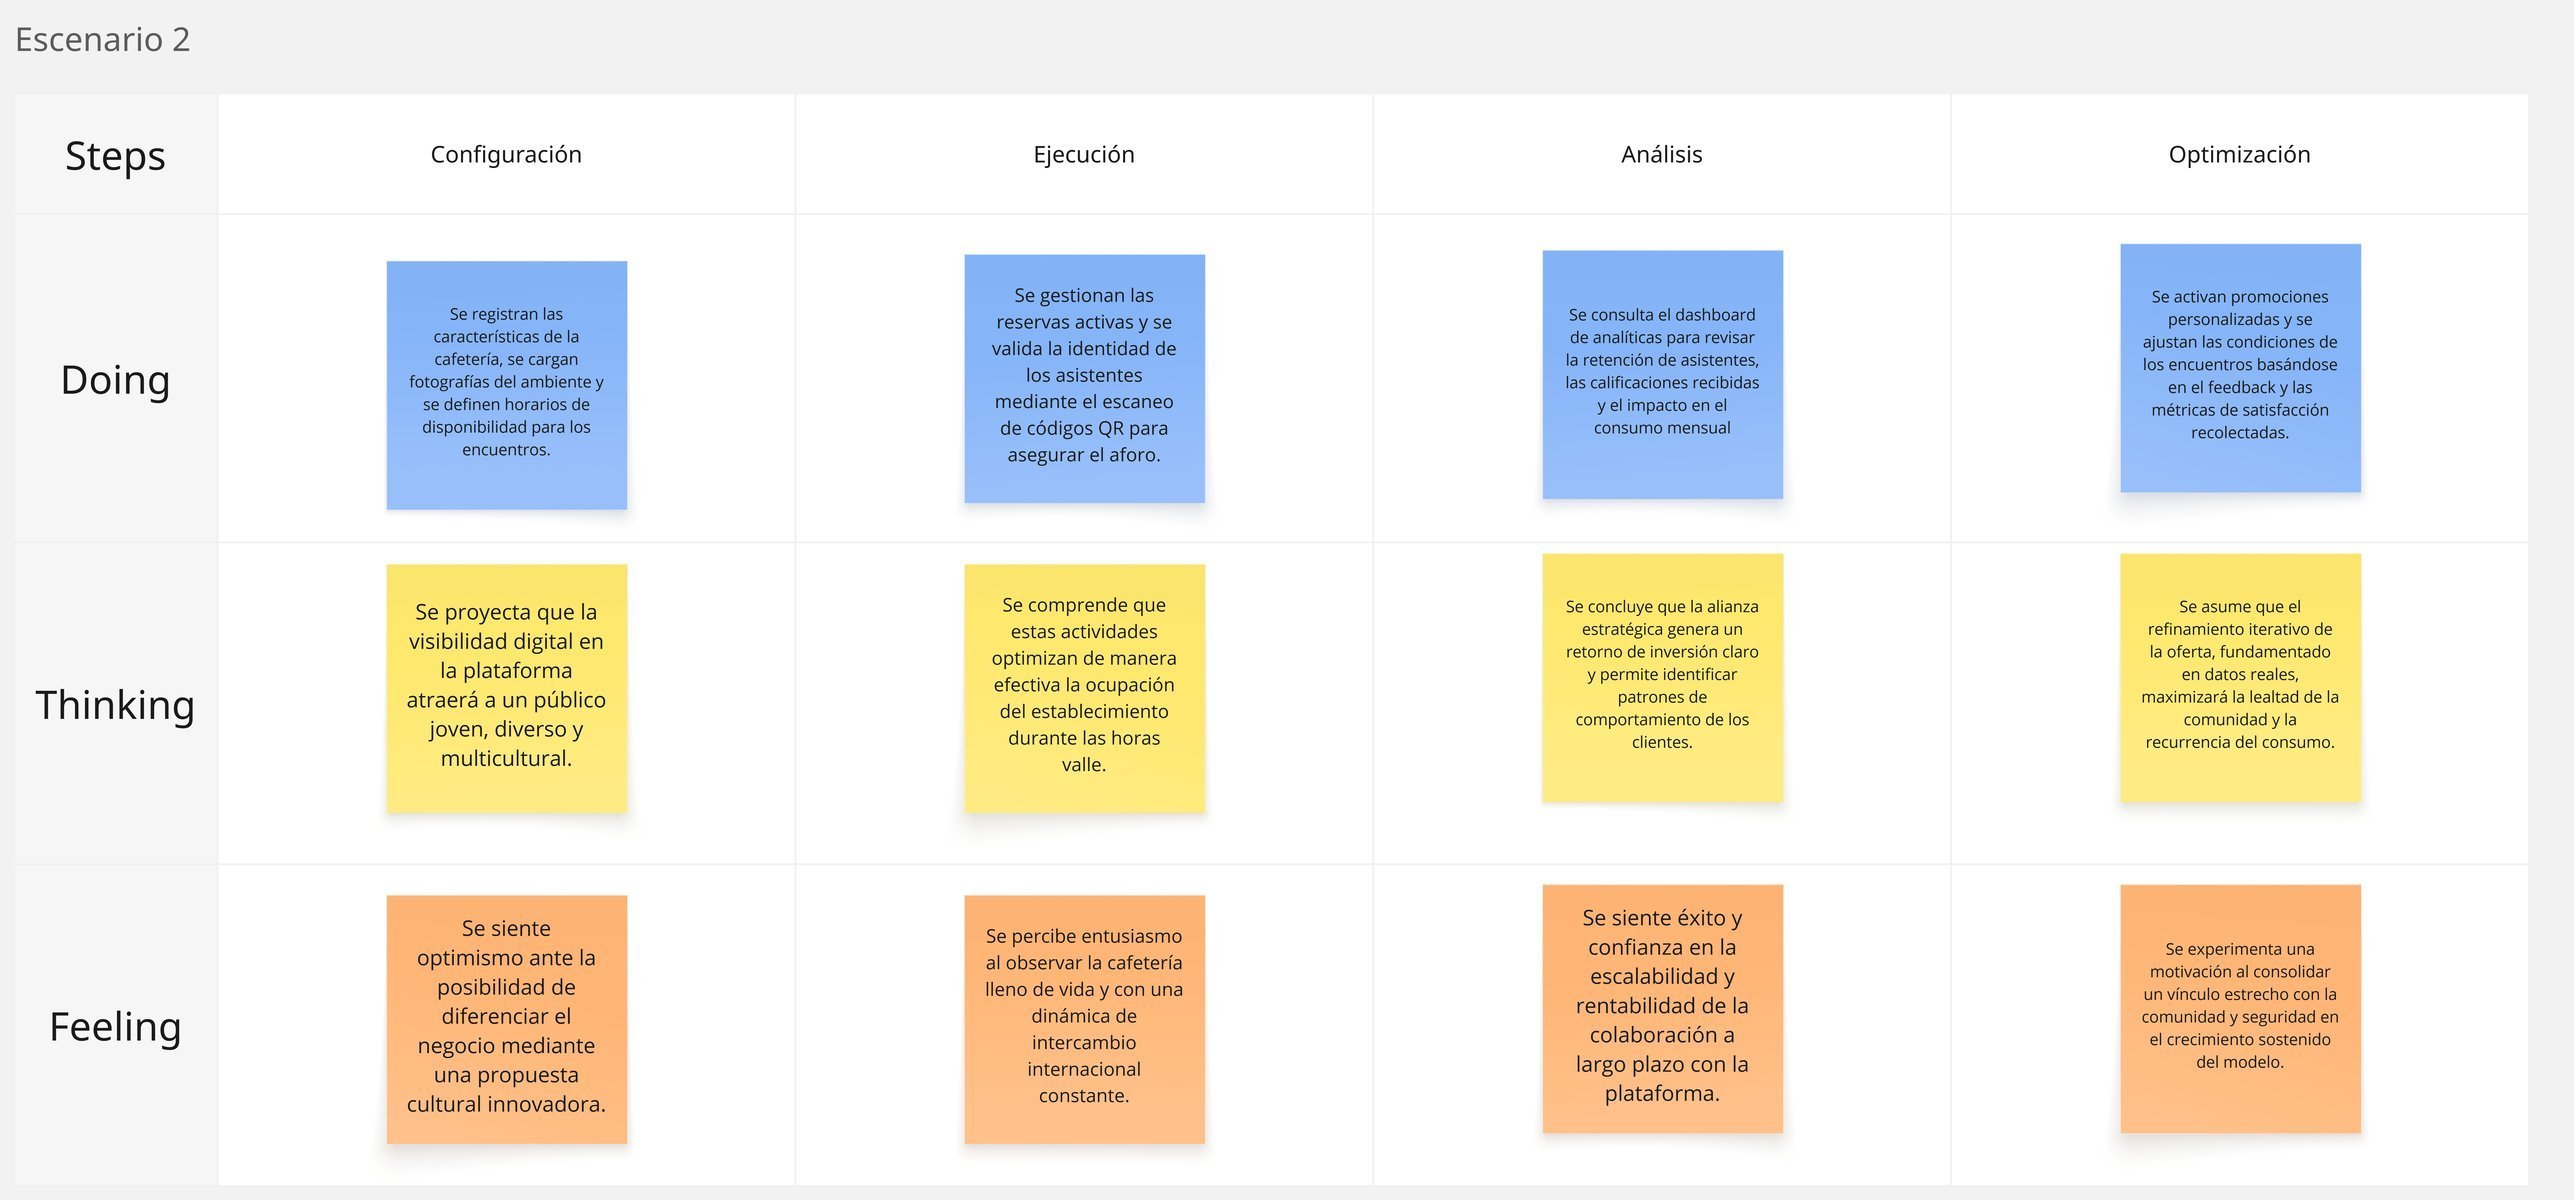
\includegraphics[keepaspectratio,alt={to-be-scenario-2}]{assets/img/cap3/to-be-scenario2.jpg}}
\caption{to-be-scenario-2}
\end{figure}

Este escenario detalla la interacción de los negocios asociados
(cafeterías) con la plataforma. Inicia con la configuración del perfil y
disponibilidad del local, seguido por la gestión y validación de
reservas durante los encuentros. Adicionalmente, incluye el análisis de
métricas mediante un panel de control (dashboard) y culmina con la
optimización de la oferta a través de promociones basadas en datos. El
objetivo principal es maximizar la ocupación en horas valle, incrementar
la rentabilidad y fidelizar a una nueva clientela.

\subsection{3.2 User
Stories}\label{report__30-cap3-requirements-spec.md__user-stories}

\subsection{Tabla de User Stories de Landing
Page}\label{report__30-cap3-requirements-spec.md__tabla-de-user-stories-de-landing-page}

{\def\LTcaptype{none} % do not increment counter
\begin{longtable}[]{@{}
  >{\raggedright\arraybackslash}p{(\linewidth - 6\tabcolsep) * \real{0.2500}}
  >{\raggedright\arraybackslash}p{(\linewidth - 6\tabcolsep) * \real{0.2500}}
  >{\raggedright\arraybackslash}p{(\linewidth - 6\tabcolsep) * \real{0.2500}}
  >{\raggedright\arraybackslash}p{(\linewidth - 6\tabcolsep) * \real{0.2500}}@{}}
\toprule\noalign{}
\begin{minipage}[b]{\linewidth}\raggedright
Story ID
\end{minipage} & \begin{minipage}[b]{\linewidth}\raggedright
User
\end{minipage} & \begin{minipage}[b]{\linewidth}\raggedright
Story Points
\end{minipage} & \begin{minipage}[b]{\linewidth}\raggedright
Epic
\end{minipage} \\
\midrule\noalign{}
\endhead
\bottomrule\noalign{}
\endlastfoot
US-LP-01 & Visitante de la página & 3 & Landing Page \\
\textbf{Título} & \textbf{Visualización de la Propuesta de Valor} & & \\
\textbf{Descripción} & \textbf{Como} visitante de la página
\textbf{Quiero} ver una sección principal atractiva que resuma la idea
del producto \textbf{Para} entender rápidamente de qué se trata el
servicio. \textbf{Escenario \#1: Presentación del propósito de Glottia}
- Dado que un visitante accede a la landing page, Cuando la carga
inicial se completa, Entonces se muestra un título claro que comunica el
propósito: ``Practica idiomas cara a cara'', un subtítulo que resume el
valor principal, y una llamada a la acción para registrarse. & & \\
\end{longtable}
}

{\def\LTcaptype{none} % do not increment counter
\begin{longtable}[]{@{}
  >{\raggedright\arraybackslash}p{(\linewidth - 6\tabcolsep) * \real{0.2500}}
  >{\raggedright\arraybackslash}p{(\linewidth - 6\tabcolsep) * \real{0.2500}}
  >{\raggedright\arraybackslash}p{(\linewidth - 6\tabcolsep) * \real{0.2500}}
  >{\raggedright\arraybackslash}p{(\linewidth - 6\tabcolsep) * \real{0.2500}}@{}}
\toprule\noalign{}
\begin{minipage}[b]{\linewidth}\raggedright
Story ID
\end{minipage} & \begin{minipage}[b]{\linewidth}\raggedright
User
\end{minipage} & \begin{minipage}[b]{\linewidth}\raggedright
Story Points
\end{minipage} & \begin{minipage}[b]{\linewidth}\raggedright
Epic
\end{minipage} \\
\midrule\noalign{}
\endhead
\bottomrule\noalign{}
\endlastfoot
US-LP-02 & Visitante interesado en practicar idiomas & 2 & Landing
Page \\
\textbf{Título} & \textbf{Ver Beneficios para Aprendices} & & \\
\textbf{Descripción} & \textbf{Como} visitante interesado en practicar
idiomas \textbf{Quiero} ver claramente los beneficios específicos para
aprendices \textbf{Para} entender cómo Glottia me puede ayudar a
mejorar. \textbf{Escenario \#1: Visualización de beneficios para
aprendices} - Dado que un visitante explora la landing page, Cuando se
desplaza a la sección de ``Para Aprendices'', Entonces identifica
claramente beneficios como ``Gana fluidez en conversaciones reales'',
``Conoce gente nueva'' y ``Acceso accesible sin academias'', cada uno
con una descripción breve. & & \\
\end{longtable}
}

{\def\LTcaptype{none} % do not increment counter
\begin{longtable}[]{@{}
  >{\raggedright\arraybackslash}p{(\linewidth - 6\tabcolsep) * \real{0.2500}}
  >{\raggedright\arraybackslash}p{(\linewidth - 6\tabcolsep) * \real{0.2500}}
  >{\raggedright\arraybackslash}p{(\linewidth - 6\tabcolsep) * \real{0.2500}}
  >{\raggedright\arraybackslash}p{(\linewidth - 6\tabcolsep) * \real{0.2500}}@{}}
\toprule\noalign{}
\begin{minipage}[b]{\linewidth}\raggedright
Story ID
\end{minipage} & \begin{minipage}[b]{\linewidth}\raggedright
User
\end{minipage} & \begin{minipage}[b]{\linewidth}\raggedright
Story Points
\end{minipage} & \begin{minipage}[b]{\linewidth}\raggedright
Epic
\end{minipage} \\
\midrule\noalign{}
\endhead
\bottomrule\noalign{}
\endlastfoot
US-LP-03 & Dueño de un local & 2 & Landing Page \\
\textbf{Título} & \textbf{Ver Beneficios para Locales} & & \\
\textbf{Descripción} & \textbf{Como} dueño de un local \textbf{Quiero}
ver claramente los beneficios que la plataforma ofrece a mi negocio
\textbf{Para} comprender cómo puede aumentar mis clientes y visibilidad.
\textbf{Escenario \#1: Visualización de beneficios para locales} - Dado
que un dueño de un local visita la landing page, Cuando navega a la
sección de ``Para Locales'', Entonces ve beneficios destacados como
``Atrae nuevos clientes'', ``Aumenta el consumo en horas valle'' y
``Publicidad gratuita para tu negocio''. & & \\
\end{longtable}
}

{\def\LTcaptype{none} % do not increment counter
\begin{longtable}[]{@{}
  >{\raggedright\arraybackslash}p{(\linewidth - 6\tabcolsep) * \real{0.2500}}
  >{\raggedright\arraybackslash}p{(\linewidth - 6\tabcolsep) * \real{0.2500}}
  >{\raggedright\arraybackslash}p{(\linewidth - 6\tabcolsep) * \real{0.2500}}
  >{\raggedright\arraybackslash}p{(\linewidth - 6\tabcolsep) * \real{0.2500}}@{}}
\toprule\noalign{}
\begin{minipage}[b]{\linewidth}\raggedright
Story ID
\end{minipage} & \begin{minipage}[b]{\linewidth}\raggedright
User
\end{minipage} & \begin{minipage}[b]{\linewidth}\raggedright
Story Points
\end{minipage} & \begin{minipage}[b]{\linewidth}\raggedright
Epic
\end{minipage} \\
\midrule\noalign{}
\endhead
\bottomrule\noalign{}
\endlastfoot
US-LP-04 & Visitante & 3 & Landing Page \\
\textbf{Título} & \textbf{Explicación de Cómo Funciona} & & \\
\textbf{Descripción} & \textbf{Como} visitante \textbf{Quiero} ver una
explicación sencilla y visual de cómo funciona la plataforma
\textbf{Para} entender los pasos necesarios para participar.
\textbf{Escenario \#1: Pasos para el aprendiz} - Dado que un visitante
está en la sección ``Cómo Funciona'', Cuando revisa el flujo para
aprendices, Entonces ve una secuencia de 3 o 4 pasos sencillos, como
``1. Regístrate y completa tu perfil'', ``2. Busca un encuentro'' y ``3.
¡Asiste y practica!''. \textbf{Escenario \#2: Pasos para el local} -
Dado que un visitante está en la sección ``Cómo Funciona'', Cuando
revisa el flujo para locales, Entonces ve los pasos correspondientes:
``1. Registra tu local'', ``2. Ofrece tu espacio'' y ``3. Recibe a los
practicantes''. & & \\
\end{longtable}
}

{\def\LTcaptype{none} % do not increment counter
\begin{longtable}[]{@{}
  >{\raggedright\arraybackslash}p{(\linewidth - 6\tabcolsep) * \real{0.2500}}
  >{\raggedright\arraybackslash}p{(\linewidth - 6\tabcolsep) * \real{0.2500}}
  >{\raggedright\arraybackslash}p{(\linewidth - 6\tabcolsep) * \real{0.2500}}
  >{\raggedright\arraybackslash}p{(\linewidth - 6\tabcolsep) * \real{0.2500}}@{}}
\toprule\noalign{}
\begin{minipage}[b]{\linewidth}\raggedright
Story ID
\end{minipage} & \begin{minipage}[b]{\linewidth}\raggedright
User
\end{minipage} & \begin{minipage}[b]{\linewidth}\raggedright
Story Points
\end{minipage} & \begin{minipage}[b]{\linewidth}\raggedright
Epic
\end{minipage} \\
\midrule\noalign{}
\endhead
\bottomrule\noalign{}
\endlastfoot
US-LP-05 & Visitante indeciso & 3 & Landing Page \\
\textbf{Título} & \textbf{Visualización de Testimonios} & & \\
\textbf{Descripción} & \textbf{Como} visitante indeciso \textbf{Quiero}
ver testimonios de aprendices y dueños de locales reales \textbf{Para}
aumentar mi confianza en el servicio. \textbf{Escenario \#1:
Visualización de testimonios diversos} - Dado que el visitante explora
la landing page, Cuando accede a la sección de testimonios, Entonces
debe ver al menos un testimonio de un aprendiz y uno de un dueño de
local, mostrando su nombre, una foto, su rol y su comentario. & & \\
\end{longtable}
}

{\def\LTcaptype{none} % do not increment counter
\begin{longtable}[]{@{}
  >{\raggedright\arraybackslash}p{(\linewidth - 6\tabcolsep) * \real{0.2500}}
  >{\raggedright\arraybackslash}p{(\linewidth - 6\tabcolsep) * \real{0.2500}}
  >{\raggedright\arraybackslash}p{(\linewidth - 6\tabcolsep) * \real{0.2500}}
  >{\raggedright\arraybackslash}p{(\linewidth - 6\tabcolsep) * \real{0.2500}}@{}}
\toprule\noalign{}
\begin{minipage}[b]{\linewidth}\raggedright
Story ID
\end{minipage} & \begin{minipage}[b]{\linewidth}\raggedright
User
\end{minipage} & \begin{minipage}[b]{\linewidth}\raggedright
Story Points
\end{minipage} & \begin{minipage}[b]{\linewidth}\raggedright
Epic
\end{minipage} \\
\midrule\noalign{}
\endhead
\bottomrule\noalign{}
\endlastfoot
US-LP-06 & Visitante & 2 & Landing Page \\
\textbf{Título} & \textbf{Llamadas a la Acción (CTA) Diferenciadas} &
& \\
\textbf{Descripción} & \textbf{Como} visitante \textbf{Quiero} ver
botones de llamada a la acción claros y separados, uno para aprendices y
otro para locales \textbf{Para} poder registrarme fácilmente según mi
interés. \textbf{Escenario \#1: Registro como aprendiz} - Dado que un
visitante está interesado en practicar idiomas, Cuando hace clic en el
botón ``Únete como Aprendiz'', Entonces es redirigido a la página de
registro para usuarios aprendices. \textbf{Escenario \#2: Registro como
local} - Dado que un visitante es dueño de un local, Cuando hace clic en
el botón ``Registra tu Local'', Entonces es redirigido a la página de
registro para partners. & & \\
\end{longtable}
}

{\def\LTcaptype{none} % do not increment counter
\begin{longtable}[]{@{}
  >{\raggedright\arraybackslash}p{(\linewidth - 6\tabcolsep) * \real{0.2500}}
  >{\raggedright\arraybackslash}p{(\linewidth - 6\tabcolsep) * \real{0.2500}}
  >{\raggedright\arraybackslash}p{(\linewidth - 6\tabcolsep) * \real{0.2500}}
  >{\raggedright\arraybackslash}p{(\linewidth - 6\tabcolsep) * \real{0.2500}}@{}}
\toprule\noalign{}
\begin{minipage}[b]{\linewidth}\raggedright
Story ID
\end{minipage} & \begin{minipage}[b]{\linewidth}\raggedright
User
\end{minipage} & \begin{minipage}[b]{\linewidth}\raggedright
Story Points
\end{minipage} & \begin{minipage}[b]{\linewidth}\raggedright
Epic
\end{minipage} \\
\midrule\noalign{}
\endhead
\bottomrule\noalign{}
\endlastfoot
US-LP-07 & Visitante que accede desde diferentes dispositivos & 5 &
Landing Page \\
\textbf{Título} & \textbf{Adaptabilidad a Diferentes Dispositivos
(Responsive)} & & \\
\textbf{Descripción} & \textbf{Como} visitante que accede desde
diferentes dispositivos \textbf{Quiero} que la landing page se adapte
correctamente a mi pantalla \textbf{Para} tener una experiencia óptima
independientemente del dispositivo que use. \textbf{Escenario \#1:
Experiencia en dispositivo móvil} - Dado que un visitante accede a la
landing page desde un smartphone, Cuando la página se carga, Entonces
todos los elementos se reorganizan en una sola columna, el texto es
legible y los botones son fáciles de presionar, sin necesidad de hacer
zoom o scroll horizontal. & & \\
\end{longtable}
}

{\def\LTcaptype{none} % do not increment counter
\begin{longtable}[]{@{}
  >{\raggedright\arraybackslash}p{(\linewidth - 6\tabcolsep) * \real{0.2500}}
  >{\raggedright\arraybackslash}p{(\linewidth - 6\tabcolsep) * \real{0.2500}}
  >{\raggedright\arraybackslash}p{(\linewidth - 6\tabcolsep) * \real{0.2500}}
  >{\raggedright\arraybackslash}p{(\linewidth - 6\tabcolsep) * \real{0.2500}}@{}}
\toprule\noalign{}
\begin{minipage}[b]{\linewidth}\raggedright
Story ID
\end{minipage} & \begin{minipage}[b]{\linewidth}\raggedright
User
\end{minipage} & \begin{minipage}[b]{\linewidth}\raggedright
Story Points
\end{minipage} & \begin{minipage}[b]{\linewidth}\raggedright
Epic
\end{minipage} \\
\midrule\noalign{}
\endhead
\bottomrule\noalign{}
\endlastfoot
US-LP-08 & Visitante & 3 & Landing Page \\
\textbf{Título} & \textbf{Navegación mediante Encabezado Fijo} & & \\
\textbf{Descripción} & \textbf{Como} visitante \textbf{Quiero} un menú
de navegación claro en el encabezado que permanezca visible mientras me
desplazo \textbf{Para} acceder fácilmente a las diferentes secciones de
la página. \textbf{Escenario \#1: Acceso a secciones desde el
encabezado} - Dado que un visitante explora la landing page, Cuando hace
clic en una opción del menú de navegación (ej. ``Beneficios''), Entonces
la página se desplaza suavemente hasta esa sección, y el encabezado
permanece fijo en la parte superior de la pantalla. & & \\
\end{longtable}
}

{\def\LTcaptype{none} % do not increment counter
\begin{longtable}[]{@{}
  >{\raggedright\arraybackslash}p{(\linewidth - 6\tabcolsep) * \real{0.2500}}
  >{\raggedright\arraybackslash}p{(\linewidth - 6\tabcolsep) * \real{0.2500}}
  >{\raggedright\arraybackslash}p{(\linewidth - 6\tabcolsep) * \real{0.2500}}
  >{\raggedright\arraybackslash}p{(\linewidth - 6\tabcolsep) * \real{0.2500}}@{}}
\toprule\noalign{}
\begin{minipage}[b]{\linewidth}\raggedright
Story ID
\end{minipage} & \begin{minipage}[b]{\linewidth}\raggedright
User
\end{minipage} & \begin{minipage}[b]{\linewidth}\raggedright
Story Points
\end{minipage} & \begin{minipage}[b]{\linewidth}\raggedright
Epic
\end{minipage} \\
\midrule\noalign{}
\endhead
\bottomrule\noalign{}
\endlastfoot
US-LP-09 & Visitante con dudas & 2 & Landing Page \\
\textbf{Título} & \textbf{Visualización de una Sección de Preguntas
Frecuentes (FAQ)} & & \\
\textbf{Descripción} & \textbf{Como} visitante con dudas \textbf{Quiero}
encontrar una sección de preguntas frecuentes \textbf{Para} resolver
rápidamente mis inquietudes más comunes. \textbf{Escenario \#1: Resolver
una duda común} - Dado que un visitante se pregunta si tiene que pagar
para asistir, Cuando accede a la sección de FAQ y hace clic en la
pregunta ``¿Tiene algún costo?'', Entonces se despliega una respuesta
clara y concisa. & & \\
\end{longtable}
}

{\def\LTcaptype{none} % do not increment counter
\begin{longtable}[]{@{}
  >{\raggedright\arraybackslash}p{(\linewidth - 6\tabcolsep) * \real{0.2500}}
  >{\raggedright\arraybackslash}p{(\linewidth - 6\tabcolsep) * \real{0.2500}}
  >{\raggedright\arraybackslash}p{(\linewidth - 6\tabcolsep) * \real{0.2500}}
  >{\raggedright\arraybackslash}p{(\linewidth - 6\tabcolsep) * \real{0.2500}}@{}}
\toprule\noalign{}
\begin{minipage}[b]{\linewidth}\raggedright
Story ID
\end{minipage} & \begin{minipage}[b]{\linewidth}\raggedright
User
\end{minipage} & \begin{minipage}[b]{\linewidth}\raggedright
Story Points
\end{minipage} & \begin{minipage}[b]{\linewidth}\raggedright
Epic
\end{minipage} \\
\midrule\noalign{}
\endhead
\bottomrule\noalign{}
\endlastfoot
US-LP-10 & Visitante & 1 & Landing Page \\
\textbf{Título} & \textbf{Visualización del Pie de Página (Footer)} &
& \\
\textbf{Descripción} & \textbf{Como} visitante \textbf{Quiero} ver un
pie de página organizado con enlaces de interés \textbf{Para} encontrar
información adicional o contactar con la empresa. \textbf{Escenario \#1:
Contenido completo del pie de página} - Dado que un visitante se
desplaza hasta el final de la landing page, Cuando llega al pie de
página, Entonces debe ver enlaces a ``Términos y Condiciones'',
``Política de Privacidad'', y enlaces a las redes sociales del proyecto.
& & \\
\end{longtable}
}

\subsection{Tabla de User Stories por
Epic}\label{report__30-cap3-requirements-spec.md__tabla-de-user-stories-por-epic}

{\def\LTcaptype{none} % do not increment counter
\begin{longtable}[]{@{}
  >{\raggedright\arraybackslash}p{(\linewidth - 6\tabcolsep) * \real{0.3125}}
  >{\raggedright\arraybackslash}p{(\linewidth - 6\tabcolsep) * \real{0.1875}}
  >{\raggedright\arraybackslash}p{(\linewidth - 6\tabcolsep) * \real{0.3125}}
  >{\raggedright\arraybackslash}p{(\linewidth - 6\tabcolsep) * \real{0.1875}}@{}}
\toprule\noalign{}
\begin{minipage}[b]{\linewidth}\raggedright
Story ID
\end{minipage} & \begin{minipage}[b]{\linewidth}\raggedright
User
\end{minipage} & \begin{minipage}[b]{\linewidth}\raggedright
Story Points
\end{minipage} & \begin{minipage}[b]{\linewidth}\raggedright
Epic
\end{minipage} \\
\midrule\noalign{}
\endhead
\bottomrule\noalign{}
\endlastfoot
US01 & Persona interesada en practicar idiomas & 3 & Gestión de
Identidad y Acceso (IAM) \\
\textbf{Title} & \textbf{Registro de nuevo aprendiz} & & \\
\textbf{Description} & \textbf{Como} una persona interesada en practicar
idiomas \textbf{Quiero} registrarme en la plataforma con mi correo y
contraseña \textbf{Para} poder acceder a la comunidad y a los
encuentros. \textbf{Escenario \#1: Registro exitoso} - Dado que un nuevo
usuario desea unirse a la plataforma, Cuando proporciona los datos
requeridos para el registro y acepta los términos, Entonces el sistema
crea su cuenta, le envía una bienvenida y lo guía para completar su
perfil. & & \\
\end{longtable}
}

{\def\LTcaptype{none} % do not increment counter
\begin{longtable}[]{@{}
  >{\raggedright\arraybackslash}p{(\linewidth - 6\tabcolsep) * \real{0.3125}}
  >{\raggedright\arraybackslash}p{(\linewidth - 6\tabcolsep) * \real{0.1875}}
  >{\raggedright\arraybackslash}p{(\linewidth - 6\tabcolsep) * \real{0.3125}}
  >{\raggedright\arraybackslash}p{(\linewidth - 6\tabcolsep) * \real{0.1875}}@{}}
\toprule\noalign{}
\begin{minipage}[b]{\linewidth}\raggedright
Story ID
\end{minipage} & \begin{minipage}[b]{\linewidth}\raggedright
User
\end{minipage} & \begin{minipage}[b]{\linewidth}\raggedright
Priority
\end{minipage} & \begin{minipage}[b]{\linewidth}\raggedright
Epic
\end{minipage} \\
\midrule\noalign{}
\endhead
\bottomrule\noalign{}
\endlastfoot
US02 & Dueño de un local & 5 & Gestión de Identidad y Acceso (IAM) \\
\textbf{Title} & \textbf{Registro de nuevo local} & & \\
\textbf{Description} & \textbf{Como} dueño de un local \textbf{Quiero}
registrar mi negocio en la plataforma \textbf{Para} ofrecer mi espacio
para los encuentros y ganar visibilidad. \textbf{Escenario \#1: Registro
de local exitoso} - Dado que el dueño de un local desea unirse a la
plataforma, Cuando proporciona la información de su cuenta y los datos
de su negocio, Entonces el sistema crea una cuenta de tipo ``Partner'',
la asocia al local y le concede acceso al panel de gestión. & & \\
\end{longtable}
}

{\def\LTcaptype{none} % do not increment counter
\begin{longtable}[]{@{}
  >{\raggedright\arraybackslash}p{(\linewidth - 6\tabcolsep) * \real{0.3125}}
  >{\raggedright\arraybackslash}p{(\linewidth - 6\tabcolsep) * \real{0.1875}}
  >{\raggedright\arraybackslash}p{(\linewidth - 6\tabcolsep) * \real{0.3125}}
  >{\raggedright\arraybackslash}p{(\linewidth - 6\tabcolsep) * \real{0.1875}}@{}}
\toprule\noalign{}
\begin{minipage}[b]{\linewidth}\raggedright
Story ID
\end{minipage} & \begin{minipage}[b]{\linewidth}\raggedright
User
\end{minipage} & \begin{minipage}[b]{\linewidth}\raggedright
Priority
\end{minipage} & \begin{minipage}[b]{\linewidth}\raggedright
Epic
\end{minipage} \\
\midrule\noalign{}
\endhead
\bottomrule\noalign{}
\endlastfoot
US03 & Usuario registrado (aprendiz o dueño de local) & 3 & Gestión de
Identidad y Acceso (IAM) \\
\textbf{Title} & \textbf{Inicio de sesión general} & & \\
\textbf{Description} & \textbf{Como} usuario registrado (aprendiz o
dueño de local) \textbf{Quiero} iniciar sesión con mi correo y
contraseña \textbf{Para} acceder a mis funcionalidades personalizadas.
\textbf{Escenario \#1: Inicio de sesión exitoso} - Dado que un usuario
registrado desea acceder a su cuenta, Cuando proporciona sus
credenciales de acceso correctas, Entonces el sistema lo autentica y le
presenta su panel principal correspondiente. \textbf{Escenario \#2:
Credenciales incorrectas} - Dado que un usuario registrado desea acceder
a su cuenta, Cuando proporciona credenciales incorrectas, Entonces el
sistema le informa que el acceso ha sido denegado por credenciales
inválidas. & & \\
\end{longtable}
}

{\def\LTcaptype{none} % do not increment counter
\begin{longtable}[]{@{}
  >{\raggedright\arraybackslash}p{(\linewidth - 6\tabcolsep) * \real{0.3125}}
  >{\raggedright\arraybackslash}p{(\linewidth - 6\tabcolsep) * \real{0.1875}}
  >{\raggedright\arraybackslash}p{(\linewidth - 6\tabcolsep) * \real{0.3125}}
  >{\raggedright\arraybackslash}p{(\linewidth - 6\tabcolsep) * \real{0.1875}}@{}}
\toprule\noalign{}
\begin{minipage}[b]{\linewidth}\raggedright
Story ID
\end{minipage} & \begin{minipage}[b]{\linewidth}\raggedright
User
\end{minipage} & \begin{minipage}[b]{\linewidth}\raggedright
Priority
\end{minipage} & \begin{minipage}[b]{\linewidth}\raggedright
Epic
\end{minipage} \\
\midrule\noalign{}
\endhead
\bottomrule\noalign{}
\endlastfoot
US04 & Usuario autenticado & 1 & Gestión de Identidad y Acceso (IAM) \\
\textbf{Title} & \textbf{Cierre de sesión} & & \\
\textbf{Description} & \textbf{Como} usuario autenticado \textbf{Quiero}
poder cerrar mi sesión \textbf{Para} proteger la privacidad de mi cuenta
en dispositivos compartidos. \textbf{Escenario \#1: Cierre de sesión
exitoso} - Dado que un usuario ha iniciado sesión en la plataforma,
Cuando solicita finalizar su sesión, Entonces el sistema termina la
sesión activa y lo devuelve a la página de inicio pública. & & \\
\end{longtable}
}

{\def\LTcaptype{none} % do not increment counter
\begin{longtable}[]{@{}
  >{\raggedright\arraybackslash}p{(\linewidth - 6\tabcolsep) * \real{0.3125}}
  >{\raggedright\arraybackslash}p{(\linewidth - 6\tabcolsep) * \real{0.1875}}
  >{\raggedright\arraybackslash}p{(\linewidth - 6\tabcolsep) * \real{0.3125}}
  >{\raggedright\arraybackslash}p{(\linewidth - 6\tabcolsep) * \real{0.1875}}@{}}
\toprule\noalign{}
\begin{minipage}[b]{\linewidth}\raggedright
Story ID
\end{minipage} & \begin{minipage}[b]{\linewidth}\raggedright
User
\end{minipage} & \begin{minipage}[b]{\linewidth}\raggedright
Priority
\end{minipage} & \begin{minipage}[b]{\linewidth}\raggedright
Epic
\end{minipage} \\
\midrule\noalign{}
\endhead
\bottomrule\noalign{}
\endlastfoot
US05 & Usuario registrado & 2 & Gestión de Identidad y Acceso (IAM) \\
\textbf{Title} & \textbf{Recuperación de contraseña} & & \\
\textbf{Description} & \textbf{Como} usuario registrado \textbf{Quiero}
solicitar un enlace para restablecer mi contraseña si la he olvidado
\textbf{Para} poder recuperar el acceso a mi cuenta. \textbf{Escenario
\#1: Solicitud de recuperación exitosa} - Dado que un usuario olvidó su
contraseña, Cuando proporciona el correo electrónico de su cuenta para
la recuperación, Entonces el sistema le envía un correo con las
instrucciones para crear una nueva contraseña. & & \\
\end{longtable}
}

{\def\LTcaptype{none} % do not increment counter
\begin{longtable}[]{@{}
  >{\raggedright\arraybackslash}p{(\linewidth - 6\tabcolsep) * \real{0.3125}}
  >{\raggedright\arraybackslash}p{(\linewidth - 6\tabcolsep) * \real{0.1875}}
  >{\raggedright\arraybackslash}p{(\linewidth - 6\tabcolsep) * \real{0.3125}}
  >{\raggedright\arraybackslash}p{(\linewidth - 6\tabcolsep) * \real{0.1875}}@{}}
\toprule\noalign{}
\begin{minipage}[b]{\linewidth}\raggedright
Story ID
\end{minipage} & \begin{minipage}[b]{\linewidth}\raggedright
User
\end{minipage} & \begin{minipage}[b]{\linewidth}\raggedright
Priority
\end{minipage} & \begin{minipage}[b]{\linewidth}\raggedright
Epic
\end{minipage} \\
\midrule\noalign{}
\endhead
\bottomrule\noalign{}
\endlastfoot
US06 & Nuevo aprendiz & 3 & Perfiles de Usuario (Profiles) \\
\textbf{Title} & \textbf{Completar perfil de aprendiz} & & \\
\textbf{Description} & \textbf{Como} nuevo aprendiz \textbf{Quiero}
completar mi perfil con mi idioma nativo, los idiomas que quiero
practicar y mi nivel \textbf{Para} que otros usuarios me conozcan y el
sistema me recomiende encuentros relevantes. \textbf{Escenario \#1:
Primer llenado de perfil} - Dado que un aprendiz se ha registrado,
Cuando especifica sus idiomas, su nivel de fluidez y guarda la
información, Entonces su perfil se actualiza y el sistema utiliza estas
preferencias para recomendarle encuentros. & & \\
\end{longtable}
}

{\def\LTcaptype{none} % do not increment counter
\begin{longtable}[]{@{}
  >{\raggedright\arraybackslash}p{(\linewidth - 6\tabcolsep) * \real{0.3125}}
  >{\raggedright\arraybackslash}p{(\linewidth - 6\tabcolsep) * \real{0.1875}}
  >{\raggedright\arraybackslash}p{(\linewidth - 6\tabcolsep) * \real{0.3125}}
  >{\raggedright\arraybackslash}p{(\linewidth - 6\tabcolsep) * \real{0.1875}}@{}}
\toprule\noalign{}
\begin{minipage}[b]{\linewidth}\raggedright
Story ID
\end{minipage} & \begin{minipage}[b]{\linewidth}\raggedright
User
\end{minipage} & \begin{minipage}[b]{\linewidth}\raggedright
Priority
\end{minipage} & \begin{minipage}[b]{\linewidth}\raggedright
Epic
\end{minipage} \\
\midrule\noalign{}
\endhead
\bottomrule\noalign{}
\endlastfoot
US07 & Aprendiz & 2 & Perfiles de Usuario (Profiles) \\
\textbf{Title} & \textbf{Editar perfil de aprendiz} & & \\
\textbf{Description} & \textbf{Como} aprendiz \textbf{Quiero} poder
editar la información de mi perfil en cualquier momento \textbf{Para}
mantenerla actualizada. \textbf{Escenario \#1: Actualización de idiomas}
- Dado que un aprendiz ha mejorado su nivel de inglés, Cuando actualiza
su nivel de fluidez en su perfil, Entonces el sistema guarda los cambios
y su perfil público refleja la nueva información. & & \\
\end{longtable}
}

{\def\LTcaptype{none} % do not increment counter
\begin{longtable}[]{@{}
  >{\raggedright\arraybackslash}p{(\linewidth - 6\tabcolsep) * \real{0.3125}}
  >{\raggedright\arraybackslash}p{(\linewidth - 6\tabcolsep) * \real{0.1875}}
  >{\raggedright\arraybackslash}p{(\linewidth - 6\tabcolsep) * \real{0.3125}}
  >{\raggedright\arraybackslash}p{(\linewidth - 6\tabcolsep) * \real{0.1875}}@{}}
\toprule\noalign{}
\begin{minipage}[b]{\linewidth}\raggedright
Story ID
\end{minipage} & \begin{minipage}[b]{\linewidth}\raggedright
User
\end{minipage} & \begin{minipage}[b]{\linewidth}\raggedright
Priority
\end{minipage} & \begin{minipage}[b]{\linewidth}\raggedright
Epic
\end{minipage} \\
\midrule\noalign{}
\endhead
\bottomrule\noalign{}
\endlastfoot
US08 & Aprendiz & 2 & Perfiles de Usuario (Profiles) \\
\textbf{Title} & \textbf{Ver perfil de otro usuario} & & \\
\textbf{Description} & \textbf{Como} aprendiz \textbf{Quiero} ver el
perfil de otros asistentes a un encuentro \textbf{Para} conocer sus
idiomas de interés y conectar con ellos. \textbf{Escenario \#1:
Visualización de perfil público} - Dado que estoy viendo los detalles de
un encuentro, Cuando solicito ver el perfil de otro asistente, Entonces
se me muestra su información pública relevante (foto, nombre, idiomas).
& & \\
\end{longtable}
}

{\def\LTcaptype{none} % do not increment counter
\begin{longtable}[]{@{}
  >{\raggedright\arraybackslash}p{(\linewidth - 6\tabcolsep) * \real{0.3125}}
  >{\raggedright\arraybackslash}p{(\linewidth - 6\tabcolsep) * \real{0.1875}}
  >{\raggedright\arraybackslash}p{(\linewidth - 6\tabcolsep) * \real{0.3125}}
  >{\raggedright\arraybackslash}p{(\linewidth - 6\tabcolsep) * \real{0.1875}}@{}}
\toprule\noalign{}
\begin{minipage}[b]{\linewidth}\raggedright
Story ID
\end{minipage} & \begin{minipage}[b]{\linewidth}\raggedright
User
\end{minipage} & \begin{minipage}[b]{\linewidth}\raggedright
Priority
\end{minipage} & \begin{minipage}[b]{\linewidth}\raggedright
Epic
\end{minipage} \\
\midrule\noalign{}
\endhead
\bottomrule\noalign{}
\endlastfoot
US09 & Usuario & 2 & Perfiles de Usuario (Profiles) \\
\textbf{Title} & \textbf{Subir foto de perfil} & & \\
\textbf{Description} & \textbf{Como} usuario \textbf{Quiero} subir una
foto de perfil \textbf{Para} personalizar mi cuenta y que otros me
reconozcan más fácilmente. \textbf{Escenario \#1: Carga de imagen
exitosa} - Dado que estoy gestionando mi perfil, Cuando proporciono una
nueva imagen para mi perfil, Entonces la imagen se actualiza y se
muestra en toda la plataforma. & & \\
\end{longtable}
}

{\def\LTcaptype{none} % do not increment counter
\begin{longtable}[]{@{}
  >{\raggedright\arraybackslash}p{(\linewidth - 6\tabcolsep) * \real{0.3125}}
  >{\raggedright\arraybackslash}p{(\linewidth - 6\tabcolsep) * \real{0.1875}}
  >{\raggedright\arraybackslash}p{(\linewidth - 6\tabcolsep) * \real{0.3125}}
  >{\raggedright\arraybackslash}p{(\linewidth - 6\tabcolsep) * \real{0.1875}}@{}}
\toprule\noalign{}
\begin{minipage}[b]{\linewidth}\raggedright
Story ID
\end{minipage} & \begin{minipage}[b]{\linewidth}\raggedright
User
\end{minipage} & \begin{minipage}[b]{\linewidth}\raggedright
Priority
\end{minipage} & \begin{minipage}[b]{\linewidth}\raggedright
Epic
\end{minipage} \\
\midrule\noalign{}
\endhead
\bottomrule\noalign{}
\endlastfoot
US10 & Dueño de negocio (Partner) & 5 & Gestión de Locales (Partner) \\
\textbf{Title} & \textbf{Dar de alta un nuevo local} & & \\
\textbf{Description} & \textbf{Como} dueño de negocio (Partner)
\textbf{Quiero} añadir los detalles de mi local, incluyendo nombre,
dirección, aforo y horario \textbf{Para} que aparezca en la plataforma
como un lugar disponible para encuentros. \textbf{Escenario \#1:
Registro de información del local} - Dado que un Partner desea añadir un
nuevo local, Cuando proporciona toda la información requerida del
establecimiento y la guarda, Entonces el local se añade a su perfil y se
vuelve visible en la plataforma. & & \\
\end{longtable}
}

{\def\LTcaptype{none} % do not increment counter
\begin{longtable}[]{@{}
  >{\raggedright\arraybackslash}p{(\linewidth - 6\tabcolsep) * \real{0.3125}}
  >{\raggedright\arraybackslash}p{(\linewidth - 6\tabcolsep) * \real{0.1875}}
  >{\raggedright\arraybackslash}p{(\linewidth - 6\tabcolsep) * \real{0.3125}}
  >{\raggedright\arraybackslash}p{(\linewidth - 6\tabcolsep) * \real{0.1875}}@{}}
\toprule\noalign{}
\begin{minipage}[b]{\linewidth}\raggedright
Story ID
\end{minipage} & \begin{minipage}[b]{\linewidth}\raggedright
User
\end{minipage} & \begin{minipage}[b]{\linewidth}\raggedright
Priority
\end{minipage} & \begin{minipage}[b]{\linewidth}\raggedright
Epic
\end{minipage} \\
\midrule\noalign{}
\endhead
\bottomrule\noalign{}
\endlastfoot
US11 & Partner & 3 & Gestión de Locales (Partner) \\
\textbf{Title} & \textbf{Editar información de un local} & & \\
\textbf{Description} & \textbf{Como} Partner \textbf{Quiero} poder
editar los detalles de mi local registrado \textbf{Para} mantener la
información actualizada (ej. cambio de horario). \textbf{Escenario \#1:
Actualizar horario del local} - Dado que un Partner necesita cambiar el
horario de su cafetería, Cuando modifica la información del horario en
los detalles del local, Entonces la nueva información se refleja
inmediatamente en la plataforma. & & \\
\end{longtable}
}

{\def\LTcaptype{none} % do not increment counter
\begin{longtable}[]{@{}
  >{\raggedright\arraybackslash}p{(\linewidth - 6\tabcolsep) * \real{0.3125}}
  >{\raggedright\arraybackslash}p{(\linewidth - 6\tabcolsep) * \real{0.1875}}
  >{\raggedright\arraybackslash}p{(\linewidth - 6\tabcolsep) * \real{0.3125}}
  >{\raggedright\arraybackslash}p{(\linewidth - 6\tabcolsep) * \real{0.1875}}@{}}
\toprule\noalign{}
\begin{minipage}[b]{\linewidth}\raggedright
Story ID
\end{minipage} & \begin{minipage}[b]{\linewidth}\raggedright
User
\end{minipage} & \begin{minipage}[b]{\linewidth}\raggedright
Priority
\end{minipage} & \begin{minipage}[b]{\linewidth}\raggedright
Epic
\end{minipage} \\
\midrule\noalign{}
\endhead
\bottomrule\noalign{}
\endlastfoot
US12 & Partner & 3 & Gestión de Locales (Partner) \\
\textbf{Title} & \textbf{Añadir fotos del local} & & \\
\textbf{Description} & \textbf{Como} Partner \textbf{Quiero} subir
varias fotos de mi local \textbf{Para} hacerlo más atractivo y mostrar
el ambiente a los aprendices. \textbf{Escenario \#1: Cargar galería de
fotos} - Dado que un Partner está gestionando el perfil de su local,
Cuando proporciona un conjunto de imágenes del establecimiento, Entonces
las fotos se asocian al perfil del local y se muestran en una galería. &
& \\
\end{longtable}
}

{\def\LTcaptype{none} % do not increment counter
\begin{longtable}[]{@{}
  >{\raggedright\arraybackslash}p{(\linewidth - 6\tabcolsep) * \real{0.3125}}
  >{\raggedright\arraybackslash}p{(\linewidth - 6\tabcolsep) * \real{0.1875}}
  >{\raggedright\arraybackslash}p{(\linewidth - 6\tabcolsep) * \real{0.3125}}
  >{\raggedright\arraybackslash}p{(\linewidth - 6\tabcolsep) * \real{0.1875}}@{}}
\toprule\noalign{}
\begin{minipage}[b]{\linewidth}\raggedright
Story ID
\end{minipage} & \begin{minipage}[b]{\linewidth}\raggedright
User
\end{minipage} & \begin{minipage}[b]{\linewidth}\raggedright
Priority
\end{minipage} & \begin{minipage}[b]{\linewidth}\raggedright
Epic
\end{minipage} \\
\midrule\noalign{}
\endhead
\bottomrule\noalign{}
\endlastfoot
US13 & Partner & 2 & Gestión de Locales (Partner) \\
\textbf{Title} & \textbf{Definir consumo mínimo (Opcional)} & & \\
\textbf{Description} & \textbf{Como} Partner \textbf{Quiero} tener la
opción de definir un consumo mínimo sugerido para los asistentes a
encuentros en mi local \textbf{Para} asegurar un retorno económico.
\textbf{Escenario \#1: Establecer consumo mínimo} - Dado que un Partner
desea incentivar el consumo, Cuando establece un consumo mínimo sugerido
para los encuentros en su local, Entonces esta información es visible en
los detalles de dichos encuentros. & & \\
\end{longtable}
}

{\def\LTcaptype{none} % do not increment counter
\begin{longtable}[]{@{}
  >{\raggedright\arraybackslash}p{(\linewidth - 6\tabcolsep) * \real{0.3125}}
  >{\raggedright\arraybackslash}p{(\linewidth - 6\tabcolsep) * \real{0.1875}}
  >{\raggedright\arraybackslash}p{(\linewidth - 6\tabcolsep) * \real{0.3125}}
  >{\raggedright\arraybackslash}p{(\linewidth - 6\tabcolsep) * \real{0.1875}}@{}}
\toprule\noalign{}
\begin{minipage}[b]{\linewidth}\raggedright
Story ID
\end{minipage} & \begin{minipage}[b]{\linewidth}\raggedright
User
\end{minipage} & \begin{minipage}[b]{\linewidth}\raggedright
Priority
\end{minipage} & \begin{minipage}[b]{\linewidth}\raggedright
Epic
\end{minipage} \\
\midrule\noalign{}
\endhead
\bottomrule\noalign{}
\endlastfoot
US14 & Partner & 5 & Gestión de Locales (Partner) \\
\textbf{Title} & \textbf{Ver dashboard de mi local} & & \\
\textbf{Description} & \textbf{Como} Partner \textbf{Quiero} acceder a
un resumen de la actividad de mi local \textbf{Para} entender
rápidamente cuántos encuentros se han realizado y cuántas personas han
asistido. \textbf{Escenario \#1: Visualización de métricas clave} - Dado
que un Partner accede a su panel, Cuando solicita ver el resumen de
actividad, Entonces se le presentan las métricas clave de sus locales
(encuentros, asistentes, calificación). & & \\
\end{longtable}
}

{\def\LTcaptype{none} % do not increment counter
\begin{longtable}[]{@{}
  >{\raggedright\arraybackslash}p{(\linewidth - 6\tabcolsep) * \real{0.3125}}
  >{\raggedright\arraybackslash}p{(\linewidth - 6\tabcolsep) * \real{0.1875}}
  >{\raggedright\arraybackslash}p{(\linewidth - 6\tabcolsep) * \real{0.3125}}
  >{\raggedright\arraybackslash}p{(\linewidth - 6\tabcolsep) * \real{0.1875}}@{}}
\toprule\noalign{}
\begin{minipage}[b]{\linewidth}\raggedright
Story ID
\end{minipage} & \begin{minipage}[b]{\linewidth}\raggedright
User
\end{minipage} & \begin{minipage}[b]{\linewidth}\raggedright
Priority
\end{minipage} & \begin{minipage}[b]{\linewidth}\raggedright
Epic
\end{minipage} \\
\midrule\noalign{}
\endhead
\bottomrule\noalign{}
\endlastfoot
US15 & Aprendiz & 3 & Gestión de Encuentros (Event) \\
\textbf{Title} & \textbf{Buscar encuentros disponibles} & & \\
\textbf{Description} & \textbf{Como} aprendiz \textbf{Quiero} buscar
encuentros usando filtros por idioma, ciudad y fecha \textbf{Para}
encontrar fácilmente una sesión de práctica que me interese.
\textbf{Escenario \#1: Búsqueda con filtros} - Dado que un aprendiz
quiere encontrar un encuentro, Cuando aplica filtros de búsqueda por
idioma, ciudad y fecha, Entonces el sistema le muestra una lista de
resultados que coinciden con sus criterios. & & \\
\end{longtable}
}

{\def\LTcaptype{none} % do not increment counter
\begin{longtable}[]{@{}
  >{\raggedright\arraybackslash}p{(\linewidth - 6\tabcolsep) * \real{0.3125}}
  >{\raggedright\arraybackslash}p{(\linewidth - 6\tabcolsep) * \real{0.1875}}
  >{\raggedright\arraybackslash}p{(\linewidth - 6\tabcolsep) * \real{0.3125}}
  >{\raggedright\arraybackslash}p{(\linewidth - 6\tabcolsep) * \real{0.1875}}@{}}
\toprule\noalign{}
\begin{minipage}[b]{\linewidth}\raggedright
Story ID
\end{minipage} & \begin{minipage}[b]{\linewidth}\raggedright
User
\end{minipage} & \begin{minipage}[b]{\linewidth}\raggedright
Priority
\end{minipage} & \begin{minipage}[b]{\linewidth}\raggedright
Epic
\end{minipage} \\
\midrule\noalign{}
\endhead
\bottomrule\noalign{}
\endlastfoot
US16 & Aprendiz & 2 & Gestión de Encuentros (Event) \\
\textbf{Title} & \textbf{Ver detalles de un encuentro} & & \\
\textbf{Description} & \textbf{Como} aprendiz \textbf{Quiero} ver los
detalles completos de un encuentro \textbf{Para} saber el idioma, el
tema, el lugar, la hora y quiénes más asistirán. \textbf{Escenario \#1:
Acceder a la información del encuentro} - Dado que un aprendiz ha
encontrado un encuentro de su interés, Cuando selecciona ese encuentro
de la lista, Entonces se le presenta toda la información detallada del
evento. & & \\
\end{longtable}
}

{\def\LTcaptype{none} % do not increment counter
\begin{longtable}[]{@{}
  >{\raggedright\arraybackslash}p{(\linewidth - 6\tabcolsep) * \real{0.3125}}
  >{\raggedright\arraybackslash}p{(\linewidth - 6\tabcolsep) * \real{0.1875}}
  >{\raggedright\arraybackslash}p{(\linewidth - 6\tabcolsep) * \real{0.3125}}
  >{\raggedright\arraybackslash}p{(\linewidth - 6\tabcolsep) * \real{0.1875}}@{}}
\toprule\noalign{}
\begin{minipage}[b]{\linewidth}\raggedright
Story ID
\end{minipage} & \begin{minipage}[b]{\linewidth}\raggedright
User
\end{minipage} & \begin{minipage}[b]{\linewidth}\raggedright
Priority
\end{minipage} & \begin{minipage}[b]{\linewidth}\raggedright
Epic
\end{minipage} \\
\midrule\noalign{}
\endhead
\bottomrule\noalign{}
\endlastfoot
US17 & Aprendiz & 5 & Gestión de Encuentros (Event) \\
\textbf{Title} & \textbf{Reservar un cupo en un encuentro} & & \\
\textbf{Description} & \textbf{Como} aprendiz \textbf{Quiero} reservar
mi cupo en un encuentro que tenga plazas disponibles \textbf{Para}
asegurar mi asistencia. \textbf{Escenario \#1: Reserva exitosa} - Dado
que un aprendiz está viendo un encuentro con cupos disponibles, Cuando
confirma su deseo de reservar un cupo, Entonces el sistema procesa su
reserva, actualiza los cupos y le envía una notificación. & & \\
\end{longtable}
}

{\def\LTcaptype{none} % do not increment counter
\begin{longtable}[]{@{}
  >{\raggedright\arraybackslash}p{(\linewidth - 6\tabcolsep) * \real{0.3125}}
  >{\raggedright\arraybackslash}p{(\linewidth - 6\tabcolsep) * \real{0.1875}}
  >{\raggedright\arraybackslash}p{(\linewidth - 6\tabcolsep) * \real{0.3125}}
  >{\raggedright\arraybackslash}p{(\linewidth - 6\tabcolsep) * \real{0.1875}}@{}}
\toprule\noalign{}
\begin{minipage}[b]{\linewidth}\raggedright
Story ID
\end{minipage} & \begin{minipage}[b]{\linewidth}\raggedright
User
\end{minipage} & \begin{minipage}[b]{\linewidth}\raggedright
Priority
\end{minipage} & \begin{minipage}[b]{\linewidth}\raggedright
Epic
\end{minipage} \\
\midrule\noalign{}
\endhead
\bottomrule\noalign{}
\endlastfoot
US18 & Aprendiz & 5 & Gestión de Encuentros (Event) \\
\textbf{Title} & \textbf{Recibir confirmación con código QR} & & \\
\textbf{Description} & \textbf{Como} aprendiz \textbf{Quiero} recibir
una confirmación de mi reserva \textbf{Para} poder hacer check-in
fácilmente al llegar al local. \textbf{Escenario \#1: Generación de QR
tras reserva} - Dado que un aprendiz ha completado una reserva, Cuando
consulta los detalles de su reserva, Entonces el sistema le proporciona
un código QR único para el check-in. & & \\
\end{longtable}
}

{\def\LTcaptype{none} % do not increment counter
\begin{longtable}[]{@{}
  >{\raggedright\arraybackslash}p{(\linewidth - 6\tabcolsep) * \real{0.3125}}
  >{\raggedright\arraybackslash}p{(\linewidth - 6\tabcolsep) * \real{0.1875}}
  >{\raggedright\arraybackslash}p{(\linewidth - 6\tabcolsep) * \real{0.3125}}
  >{\raggedright\arraybackslash}p{(\linewidth - 6\tabcolsep) * \real{0.1875}}@{}}
\toprule\noalign{}
\begin{minipage}[b]{\linewidth}\raggedright
Story ID
\end{minipage} & \begin{minipage}[b]{\linewidth}\raggedright
User
\end{minipage} & \begin{minipage}[b]{\linewidth}\raggedright
Priority
\end{minipage} & \begin{minipage}[b]{\linewidth}\raggedright
Epic
\end{minipage} \\
\midrule\noalign{}
\endhead
\bottomrule\noalign{}
\endlastfoot
US19 & Aprendiz & 8 & Gestión de Encuentros (Event) \\
\textbf{Title} & \textbf{Crear un encuentro (iniciativa del aprendiz)} &
& \\
\textbf{Description} & \textbf{Como} aprendiz \textbf{Quiero} proponer
la creación de un nuevo encuentro en un local registrado \textbf{Para}
organizar una sesión si no hay ninguna que se ajuste a mis necesidades.
\textbf{Escenario \#1: Proponer nuevo encuentro} - Dado que un aprendiz
desea organizar un encuentro, Cuando proporciona los detalles del nuevo
evento (local, fecha, idioma), Entonces el sistema crea el encuentro, lo
registra como el primer asistente y lo hace visible para otros usuarios.
& & \\
\end{longtable}
}

{\def\LTcaptype{none} % do not increment counter
\begin{longtable}[]{@{}
  >{\raggedright\arraybackslash}p{(\linewidth - 6\tabcolsep) * \real{0.3125}}
  >{\raggedright\arraybackslash}p{(\linewidth - 6\tabcolsep) * \real{0.1875}}
  >{\raggedright\arraybackslash}p{(\linewidth - 6\tabcolsep) * \real{0.3125}}
  >{\raggedright\arraybackslash}p{(\linewidth - 6\tabcolsep) * \real{0.1875}}@{}}
\toprule\noalign{}
\begin{minipage}[b]{\linewidth}\raggedright
Story ID
\end{minipage} & \begin{minipage}[b]{\linewidth}\raggedright
User
\end{minipage} & \begin{minipage}[b]{\linewidth}\raggedright
Priority
\end{minipage} & \begin{minipage}[b]{\linewidth}\raggedright
Epic
\end{minipage} \\
\midrule\noalign{}
\endhead
\bottomrule\noalign{}
\endlastfoot
US20 & Aprendiz & 8 & Gestión de Encuentros (Event) \\
\textbf{Title} & \textbf{Check-in en un encuentro} & & \\
\textbf{Description} & \textbf{Como} aprendiz \textbf{Quiero} confirmar
mi asistencia a un encuentro \textbf{Para} para registrar mi
participación y recebir los beneficios por ello. \textbf{Escenario \#1:
Check-in exitoso por parte del local} - Dado que un aprendiz llega al
local del encuentro, Cuando su código QR es validado por el organizador,
Entonces el sistema registra su asistencia y le asigna los puntos
correspondientes. & & \\
\end{longtable}
}

{\def\LTcaptype{none} % do not increment counter
\begin{longtable}[]{@{}
  >{\raggedright\arraybackslash}p{(\linewidth - 6\tabcolsep) * \real{0.3125}}
  >{\raggedright\arraybackslash}p{(\linewidth - 6\tabcolsep) * \real{0.1875}}
  >{\raggedright\arraybackslash}p{(\linewidth - 6\tabcolsep) * \real{0.3125}}
  >{\raggedright\arraybackslash}p{(\linewidth - 6\tabcolsep) * \real{0.1875}}@{}}
\toprule\noalign{}
\begin{minipage}[b]{\linewidth}\raggedright
Story ID
\end{minipage} & \begin{minipage}[b]{\linewidth}\raggedright
User
\end{minipage} & \begin{minipage}[b]{\linewidth}\raggedright
Priority
\end{minipage} & \begin{minipage}[b]{\linewidth}\raggedright
Epic
\end{minipage} \\
\midrule\noalign{}
\endhead
\bottomrule\noalign{}
\endlastfoot
US21 & Partner & 3 & Gestión de Encuentros (Event) \\
\textbf{Title} & \textbf{Ver lista de asistentes (vista de Partner)} &
& \\
\textbf{Description} & \textbf{Como} Partner \textbf{Quiero} ver la
lista de personas que han reservado para un encuentro en mi local
\textbf{Para} tener una idea del aforo esperado. \textbf{Escenario \#1:
Consultar asistentes} - Dado que un Partner tiene un encuentro
programado, Cuando consulta los detalles de dicho evento, Entonces el
sistema le muestra la lista de los aprendices que han confirmado su
asistencia. & & \\
\end{longtable}
}

{\def\LTcaptype{none} % do not increment counter
\begin{longtable}[]{@{}
  >{\raggedright\arraybackslash}p{(\linewidth - 6\tabcolsep) * \real{0.3125}}
  >{\raggedright\arraybackslash}p{(\linewidth - 6\tabcolsep) * \real{0.1875}}
  >{\raggedright\arraybackslash}p{(\linewidth - 6\tabcolsep) * \real{0.3125}}
  >{\raggedright\arraybackslash}p{(\linewidth - 6\tabcolsep) * \real{0.1875}}@{}}
\toprule\noalign{}
\begin{minipage}[b]{\linewidth}\raggedright
Story ID
\end{minipage} & \begin{minipage}[b]{\linewidth}\raggedright
User
\end{minipage} & \begin{minipage}[b]{\linewidth}\raggedright
Priority
\end{minipage} & \begin{minipage}[b]{\linewidth}\raggedright
Epic
\end{minipage} \\
\midrule\noalign{}
\endhead
\bottomrule\noalign{}
\endlastfoot
US22 & Aprendiz con una reserva & 2 & Gestión de Encuentros (Event) \\
\textbf{Title} & \textbf{Recibir recordatorio de encuentro} & & \\
\textbf{Description} & \textbf{Como} aprendiz con una reserva
\textbf{Quiero} recibir una notificación de recordatorio 24 horas antes
del encuentro \textbf{Para} no olvidarme de asistir. \textbf{Escenario
\#1: Notificación automática} - Dado que un aprendiz tiene una reserva
para mañana, Cuando faltan 24 horas para el evento, Entonces el sistema
le envía automáticamente un recordatorio. & & \\
\end{longtable}
}

{\def\LTcaptype{none} % do not increment counter
\begin{longtable}[]{@{}
  >{\raggedright\arraybackslash}p{(\linewidth - 6\tabcolsep) * \real{0.3125}}
  >{\raggedright\arraybackslash}p{(\linewidth - 6\tabcolsep) * \real{0.1875}}
  >{\raggedright\arraybackslash}p{(\linewidth - 6\tabcolsep) * \real{0.3125}}
  >{\raggedright\arraybackslash}p{(\linewidth - 6\tabcolsep) * \real{0.1875}}@{}}
\toprule\noalign{}
\begin{minipage}[b]{\linewidth}\raggedright
Story ID
\end{minipage} & \begin{minipage}[b]{\linewidth}\raggedright
User
\end{minipage} & \begin{minipage}[b]{\linewidth}\raggedright
Priority
\end{minipage} & \begin{minipage}[b]{\linewidth}\raggedright
Epic
\end{minipage} \\
\midrule\noalign{}
\endhead
\bottomrule\noalign{}
\endlastfoot
US23 & Aprendiz & 3 & Gestión de Encuentros (Event) \\
\textbf{Title} & \textbf{Unirse a la lista de espera} & & \\
\textbf{Description} & \textbf{Como} aprendiz \textbf{Quiero} unirme a
una lista de espera si un encuentro está lleno \textbf{Para} tener la
oportunidad de asistir si alguien cancela. \textbf{Escenario \#1:
Encuentro lleno} - Dado que un aprendiz desea asistir a un encuentro sin
cupos, Cuando opta por unirse a la lista de espera, Entonces el sistema
lo añade a la cola y le notifica su posición. & & \\
\end{longtable}
}

{\def\LTcaptype{none} % do not increment counter
\begin{longtable}[]{@{}
  >{\raggedright\arraybackslash}p{(\linewidth - 6\tabcolsep) * \real{0.3125}}
  >{\raggedright\arraybackslash}p{(\linewidth - 6\tabcolsep) * \real{0.1875}}
  >{\raggedright\arraybackslash}p{(\linewidth - 6\tabcolsep) * \real{0.3125}}
  >{\raggedright\arraybackslash}p{(\linewidth - 6\tabcolsep) * \real{0.1875}}@{}}
\toprule\noalign{}
\begin{minipage}[b]{\linewidth}\raggedright
Story ID
\end{minipage} & \begin{minipage}[b]{\linewidth}\raggedright
User
\end{minipage} & \begin{minipage}[b]{\linewidth}\raggedright
Priority
\end{minipage} & \begin{minipage}[b]{\linewidth}\raggedright
Epic
\end{minipage} \\
\midrule\noalign{}
\endhead
\bottomrule\noalign{}
\endlastfoot
US24 & Aprendiz en una lista de espera & 5 & Gestión de Encuentros
(Event) \\
\textbf{Title} & \textbf{Recibir notificación de cupo liberado} & & \\
\textbf{Description} & \textbf{Como} aprendiz en una lista de espera
\textbf{Quiero} recibir una notificación inmediata si un cupo se libera
\textbf{Para} poder reservarlo rápidamente. \textbf{Escenario \#1:
Alguien cancela} - Dado que un aprendiz está en una lista de espera y se
libera un cupo, Cuando le llega su turno, Entonces el sistema le envía
una notificación para que pueda confirmar su asistencia en un tiempo
limitado. & & \\
\end{longtable}
}

{\def\LTcaptype{none} % do not increment counter
\begin{longtable}[]{@{}
  >{\raggedright\arraybackslash}p{(\linewidth - 6\tabcolsep) * \real{0.3125}}
  >{\raggedright\arraybackslash}p{(\linewidth - 6\tabcolsep) * \real{0.1875}}
  >{\raggedright\arraybackslash}p{(\linewidth - 6\tabcolsep) * \real{0.3125}}
  >{\raggedright\arraybackslash}p{(\linewidth - 6\tabcolsep) * \real{0.1875}}@{}}
\toprule\noalign{}
\begin{minipage}[b]{\linewidth}\raggedright
Story ID
\end{minipage} & \begin{minipage}[b]{\linewidth}\raggedright
User
\end{minipage} & \begin{minipage}[b]{\linewidth}\raggedright
Priority
\end{minipage} & \begin{minipage}[b]{\linewidth}\raggedright
Epic
\end{minipage} \\
\midrule\noalign{}
\endhead
\bottomrule\noalign{}
\endlastfoot
US25 & Aprendiz que asistió a un encuentro & 3 & Gestión de Encuentros
(Event) \\
\textbf{Title} & \textbf{Dejar feedback de un encuentro} & & \\
\textbf{Description} & \textbf{Como} aprendiz que asistió a un encuentro
\textbf{Quiero} dejar una calificación y un comentario sobre mi
experiencia \textbf{Para} ayudar a otros usuarios y a los locales.
\textbf{Escenario \#1: Calificar la experiencia} - Dado que un aprendiz
ha asistido a un encuentro, Cuando proporciona una calificación y un
comentario sobre el evento, Entonces el sistema guarda su feedback y lo
asocia al encuentro y al local. & & \\
\end{longtable}
}

{\def\LTcaptype{none} % do not increment counter
\begin{longtable}[]{@{}
  >{\raggedright\arraybackslash}p{(\linewidth - 6\tabcolsep) * \real{0.3125}}
  >{\raggedright\arraybackslash}p{(\linewidth - 6\tabcolsep) * \real{0.1875}}
  >{\raggedright\arraybackslash}p{(\linewidth - 6\tabcolsep) * \real{0.3125}}
  >{\raggedright\arraybackslash}p{(\linewidth - 6\tabcolsep) * \real{0.1875}}@{}}
\toprule\noalign{}
\begin{minipage}[b]{\linewidth}\raggedright
Story ID
\end{minipage} & \begin{minipage}[b]{\linewidth}\raggedright
User
\end{minipage} & \begin{minipage}[b]{\linewidth}\raggedright
Priority
\end{minipage} & \begin{minipage}[b]{\linewidth}\raggedright
Epic
\end{minipage} \\
\midrule\noalign{}
\endhead
\bottomrule\noalign{}
\endlastfoot
US26 & Aprendiz & 3 & Gestión de Encuentros (Event) \\
\textbf{Title} & \textbf{Cancelar mi reserva} & & \\
\textbf{Description} & \textbf{Como} aprendiz \textbf{Quiero} poder
cancelar mi reserva a un encuentro con antelación \textbf{Para} liberar
mi cupo si no puedo asistir. \textbf{Escenario \#1: Cancelación a
tiempo} - Dado que un aprendiz tiene una reserva y no puede asistir,
Cuando solicita la cancelación de su reserva antes del tiempo límite,
Entonces su cupo se libera para otros usuarios. & & \\
\end{longtable}
}

{\def\LTcaptype{none} % do not increment counter
\begin{longtable}[]{@{}
  >{\raggedright\arraybackslash}p{(\linewidth - 6\tabcolsep) * \real{0.3125}}
  >{\raggedright\arraybackslash}p{(\linewidth - 6\tabcolsep) * \real{0.1875}}
  >{\raggedright\arraybackslash}p{(\linewidth - 6\tabcolsep) * \real{0.3125}}
  >{\raggedright\arraybackslash}p{(\linewidth - 6\tabcolsep) * \real{0.1875}}@{}}
\toprule\noalign{}
\begin{minipage}[b]{\linewidth}\raggedright
Story ID
\end{minipage} & \begin{minipage}[b]{\linewidth}\raggedright
User
\end{minipage} & \begin{minipage}[b]{\linewidth}\raggedright
Priority
\end{minipage} & \begin{minipage}[b]{\linewidth}\raggedright
Epic
\end{minipage} \\
\midrule\noalign{}
\endhead
\bottomrule\noalign{}
\endlastfoot
US27 & Aprendiz & 2 & Gestión de Encuentros (Event) \\
\textbf{Title} & \textbf{Ver encuentros pasados} & & \\
\textbf{Description} & \textbf{Como} aprendiz \textbf{Quiero} tener un
historial de los encuentros a los que he asistido \textbf{Para} recordar
los lugares y las fechas. \textbf{Escenario \#1: Consultar historial} -
Dado que un aprendiz quiere revisar su actividad pasada, Cuando consulta
su historial de encuentros, Entonces el sistema le muestra una lista de
todos los eventos en los que participó. & & \\
\end{longtable}
}

{\def\LTcaptype{none} % do not increment counter
\begin{longtable}[]{@{}
  >{\raggedright\arraybackslash}p{(\linewidth - 6\tabcolsep) * \real{0.3125}}
  >{\raggedright\arraybackslash}p{(\linewidth - 6\tabcolsep) * \real{0.1875}}
  >{\raggedright\arraybackslash}p{(\linewidth - 6\tabcolsep) * \real{0.3125}}
  >{\raggedright\arraybackslash}p{(\linewidth - 6\tabcolsep) * \real{0.1875}}@{}}
\toprule\noalign{}
\begin{minipage}[b]{\linewidth}\raggedright
Story ID
\end{minipage} & \begin{minipage}[b]{\linewidth}\raggedright
User
\end{minipage} & \begin{minipage}[b]{\linewidth}\raggedright
Priority
\end{minipage} & \begin{minipage}[b]{\linewidth}\raggedright
Epic
\end{minipage} \\
\midrule\noalign{}
\endhead
\bottomrule\noalign{}
\endlastfoot
US28 & Aprendiz & 5 & Gestión de Encuentros (Event) \\
\textbf{Title} & \textbf{Ver el mapa de locales} & & \\
\textbf{Description} & \textbf{Como} aprendiz \textbf{Quiero} ver
locales disponibles según mi ubicación \textbf{Para} encontrar los
lugares más cercanos donde para organizar encuentros. \textbf{Escenario
\#1: Exploración geográfica} - Dado que un aprendiz quiere descubrir
nuevos locales, Cuando explora la vista de mapa, Entonces el sistema le
muestra la ubicación de todos los locales aliados. & & \\
\end{longtable}
}

{\def\LTcaptype{none} % do not increment counter
\begin{longtable}[]{@{}
  >{\raggedright\arraybackslash}p{(\linewidth - 6\tabcolsep) * \real{0.3125}}
  >{\raggedright\arraybackslash}p{(\linewidth - 6\tabcolsep) * \real{0.1875}}
  >{\raggedright\arraybackslash}p{(\linewidth - 6\tabcolsep) * \real{0.3125}}
  >{\raggedright\arraybackslash}p{(\linewidth - 6\tabcolsep) * \real{0.1875}}@{}}
\toprule\noalign{}
\begin{minipage}[b]{\linewidth}\raggedright
Story ID
\end{minipage} & \begin{minipage}[b]{\linewidth}\raggedright
User
\end{minipage} & \begin{minipage}[b]{\linewidth}\raggedright
Priority
\end{minipage} & \begin{minipage}[b]{\linewidth}\raggedright
Epic
\end{minipage} \\
\midrule\noalign{}
\endhead
\bottomrule\noalign{}
\endlastfoot
US29 & Aprendiz & 5 & Lealtad y Gamificación (Loyalty) \\
\textbf{Title} & \textbf{Ganar puntos por asistencia} & & \\
\textbf{Description} & \textbf{Como} aprendiz \textbf{Quiero} ganar
puntos de lealtad cada vez que hago check-in en un encuentro
\textbf{Para} ser recompensado por mi participación activa.
\textbf{Escenario \#1: Acumulación de puntos} - Dado que un aprendiz ha
hecho check-in exitosamente en un evento, Cuando el sistema procesa su
asistencia, Entonces automáticamente se suman los puntos
correspondientes a su cuenta. & & \\
\end{longtable}
}

{\def\LTcaptype{none} % do not increment counter
\begin{longtable}[]{@{}
  >{\raggedright\arraybackslash}p{(\linewidth - 6\tabcolsep) * \real{0.3125}}
  >{\raggedright\arraybackslash}p{(\linewidth - 6\tabcolsep) * \real{0.1875}}
  >{\raggedright\arraybackslash}p{(\linewidth - 6\tabcolsep) * \real{0.3125}}
  >{\raggedright\arraybackslash}p{(\linewidth - 6\tabcolsep) * \real{0.1875}}@{}}
\toprule\noalign{}
\begin{minipage}[b]{\linewidth}\raggedright
Story ID
\end{minipage} & \begin{minipage}[b]{\linewidth}\raggedright
User
\end{minipage} & \begin{minipage}[b]{\linewidth}\raggedright
Priority
\end{minipage} & \begin{minipage}[b]{\linewidth}\raggedright
Epic
\end{minipage} \\
\midrule\noalign{}
\endhead
\bottomrule\noalign{}
\endlastfoot
US30 & Aprendiz & 1 & Lealtad y Gamificación (Loyalty) \\
\textbf{Title} & \textbf{Ver mi total de puntos y nivel} & & \\
\textbf{Description} & \textbf{Como} aprendiz \textbf{Quiero} poder ver
mi saldo total de puntos y mi nivel actual en mi perfil \textbf{Para}
seguir mi progreso. \textbf{Escenario \#1: Consultar progreso} - Dado
que un aprendiz accede a su perfil, Cuando consulta su progreso de
lealtad, Entonces el sistema le muestra sus puntos totales y su nivel
actual. & & \\
\end{longtable}
}

{\def\LTcaptype{none} % do not increment counter
\begin{longtable}[]{@{}
  >{\raggedright\arraybackslash}p{(\linewidth - 6\tabcolsep) * \real{0.3125}}
  >{\raggedright\arraybackslash}p{(\linewidth - 6\tabcolsep) * \real{0.1875}}
  >{\raggedright\arraybackslash}p{(\linewidth - 6\tabcolsep) * \real{0.3125}}
  >{\raggedright\arraybackslash}p{(\linewidth - 6\tabcolsep) * \real{0.1875}}@{}}
\toprule\noalign{}
\begin{minipage}[b]{\linewidth}\raggedright
Story ID
\end{minipage} & \begin{minipage}[b]{\linewidth}\raggedright
User
\end{minipage} & \begin{minipage}[b]{\linewidth}\raggedright
Priority
\end{minipage} & \begin{minipage}[b]{\linewidth}\raggedright
Epic
\end{minipage} \\
\midrule\noalign{}
\endhead
\bottomrule\noalign{}
\endlastfoot
US31 & Aprendiz & 5 & Lealtad y Gamificación (Loyalty) \\
\textbf{Title} & \textbf{Desbloquear una insignia (badge)} & & \\
\textbf{Description} & \textbf{Como} aprendiz \textbf{Quiero}
desbloquear insignias al alcanzar ciertos hitos (ej. ``Asistir a 5
encuentros de francés'') \textbf{Para} sentir que logro algo.
\textbf{Escenario \#1: Desbloqueo de insignia por asistencia} - Dado que
un aprendiz ha cumplido los requisitos para una insignia, Cuando el
sistema verifica el hito, Entonces le otorga la insignia correspondiente
y le muestra una notificación. & & \\
\end{longtable}
}

{\def\LTcaptype{none} % do not increment counter
\begin{longtable}[]{@{}
  >{\raggedright\arraybackslash}p{(\linewidth - 6\tabcolsep) * \real{0.3125}}
  >{\raggedright\arraybackslash}p{(\linewidth - 6\tabcolsep) * \real{0.1875}}
  >{\raggedright\arraybackslash}p{(\linewidth - 6\tabcolsep) * \real{0.3125}}
  >{\raggedright\arraybackslash}p{(\linewidth - 6\tabcolsep) * \real{0.1875}}@{}}
\toprule\noalign{}
\begin{minipage}[b]{\linewidth}\raggedright
Story ID
\end{minipage} & \begin{minipage}[b]{\linewidth}\raggedright
User
\end{minipage} & \begin{minipage}[b]{\linewidth}\raggedright
Priority
\end{minipage} & \begin{minipage}[b]{\linewidth}\raggedright
Epic
\end{minipage} \\
\midrule\noalign{}
\endhead
\bottomrule\noalign{}
\endlastfoot
US32 & Aprendiz & 3 & Lealtad y Gamificación (Loyalty) \\
\textbf{Title} & \textbf{Ver mis insignias desbloqueadas} & & \\
\textbf{Description} & \textbf{Como} aprendiz \textbf{Quiero} tener una
sección en mi perfil donde pueda ver todas las insignias que he ganado
\textbf{Para} mostrarlas a la comunidad. \textbf{Escenario \#1: Galería
de logros} - Dado que un aprendiz ha desbloqueado insignias, Cuando
visita un perfil (suyo o de otro usuario), Entonces puede ver la
colección de insignias ganadas. & & \\
\end{longtable}
}

{\def\LTcaptype{none} % do not increment counter
\begin{longtable}[]{@{}
  >{\raggedright\arraybackslash}p{(\linewidth - 6\tabcolsep) * \real{0.3125}}
  >{\raggedright\arraybackslash}p{(\linewidth - 6\tabcolsep) * \real{0.1875}}
  >{\raggedright\arraybackslash}p{(\linewidth - 6\tabcolsep) * \real{0.3125}}
  >{\raggedright\arraybackslash}p{(\linewidth - 6\tabcolsep) * \real{0.1875}}@{}}
\toprule\noalign{}
\begin{minipage}[b]{\linewidth}\raggedright
Story ID
\end{minipage} & \begin{minipage}[b]{\linewidth}\raggedright
User
\end{minipage} & \begin{minipage}[b]{\linewidth}\raggedright
Priority
\end{minipage} & \begin{minipage}[b]{\linewidth}\raggedright
Epic
\end{minipage} \\
\midrule\noalign{}
\endhead
\bottomrule\noalign{}
\endlastfoot
US33 & Aprendiz & 3 & Lealtad y Gamificación (Loyalty) \\
\textbf{Title} & \textbf{Ver un ranking de usuarios} & & \\
\textbf{Description} & \textbf{Como} aprendiz \textbf{Quiero} recibir y
acceder a información sobre mi progreso y compararlo con el de otros
usuarios \textbf{Para} competir de forma amistosa con otros miembros de
la comunidad. \textbf{Escenario \#1: Consultar el leaderboard} - Dado
que un aprendiz quiere ver su posición en la comunidad, Cuando accede a
la tabla de clasificación, Entonces el sistema le muestra el ranking de
usuarios basado en puntos. & & \\
\end{longtable}
}

{\def\LTcaptype{none} % do not increment counter
\begin{longtable}[]{@{}
  >{\raggedright\arraybackslash}p{(\linewidth - 6\tabcolsep) * \real{0.3125}}
  >{\raggedright\arraybackslash}p{(\linewidth - 6\tabcolsep) * \real{0.1875}}
  >{\raggedright\arraybackslash}p{(\linewidth - 6\tabcolsep) * \real{0.3125}}
  >{\raggedright\arraybackslash}p{(\linewidth - 6\tabcolsep) * \real{0.1875}}@{}}
\toprule\noalign{}
\begin{minipage}[b]{\linewidth}\raggedright
Story ID
\end{minipage} & \begin{minipage}[b]{\linewidth}\raggedright
User
\end{minipage} & \begin{minipage}[b]{\linewidth}\raggedright
Priority
\end{minipage} & \begin{minipage}[b]{\linewidth}\raggedright
Epic
\end{minipage} \\
\midrule\noalign{}
\endhead
\bottomrule\noalign{}
\endlastfoot
US34 & Aprendiz leal & 5 & Lealtad y Gamificación (Loyalty) \\
\textbf{Title} & \textbf{Recibir ofertas de locales por lealtad} & & \\
\textbf{Description} & \textbf{Como} aprendiz leal \textbf{Quiero}
recibir ofertas especiales o descuentos de los locales asociados
\textbf{Como} recompensa por mi participación. \textbf{Escenario \#1:
Recompensa de un Partner} - Dado que un aprendiz ha alcanzado un nivel
de lealtad alto, Cuando un local ofrece una recompensa para ese nivel,
Entonces el aprendiz recibe una notificación con la oferta especial. &
& \\
\end{longtable}
}

{\def\LTcaptype{none} % do not increment counter
\begin{longtable}[]{@{}
  >{\raggedright\arraybackslash}p{(\linewidth - 6\tabcolsep) * \real{0.3125}}
  >{\raggedright\arraybackslash}p{(\linewidth - 6\tabcolsep) * \real{0.1875}}
  >{\raggedright\arraybackslash}p{(\linewidth - 6\tabcolsep) * \real{0.3125}}
  >{\raggedright\arraybackslash}p{(\linewidth - 6\tabcolsep) * \real{0.1875}}@{}}
\toprule\noalign{}
\begin{minipage}[b]{\linewidth}\raggedright
Story ID
\end{minipage} & \begin{minipage}[b]{\linewidth}\raggedright
User
\end{minipage} & \begin{minipage}[b]{\linewidth}\raggedright
Priority
\end{minipage} & \begin{minipage}[b]{\linewidth}\raggedright
Epic
\end{minipage} \\
\midrule\noalign{}
\endhead
\bottomrule\noalign{}
\endlastfoot
US35 & Aprendiz & 3 & Lealtad y Gamificación (Loyalty) \\
\textbf{Title} & \textbf{Mantener una racha de asistencia} & & \\
\textbf{Description} & \textbf{Como} aprendiz \textbf{Quiero} que el
sistema registre mi racha de asistencia semanal \textbf{Para} motivarme
a participar de forma consistente. \textbf{Escenario \#1: Incrementar la
racha} - Dado que un aprendiz asistió a un encuentro la semana pasada,
Cuando asiste a otro encuentro esta semana, Entonces el sistema
incrementa su racha de asistencia y se lo notifica. & & \\
\end{longtable}
}

{\def\LTcaptype{none} % do not increment counter
\begin{longtable}[]{@{}
  >{\raggedright\arraybackslash}p{(\linewidth - 6\tabcolsep) * \real{0.3125}}
  >{\raggedright\arraybackslash}p{(\linewidth - 6\tabcolsep) * \real{0.1875}}
  >{\raggedright\arraybackslash}p{(\linewidth - 6\tabcolsep) * \real{0.3125}}
  >{\raggedright\arraybackslash}p{(\linewidth - 6\tabcolsep) * \real{0.1875}}@{}}
\toprule\noalign{}
\begin{minipage}[b]{\linewidth}\raggedright
Story ID
\end{minipage} & \begin{minipage}[b]{\linewidth}\raggedright
User
\end{minipage} & \begin{minipage}[b]{\linewidth}\raggedright
Priority
\end{minipage} & \begin{minipage}[b]{\linewidth}\raggedright
Epic
\end{minipage} \\
\midrule\noalign{}
\endhead
\bottomrule\noalign{}
\endlastfoot
US36 & Partner & 5 & Analíticas (Analytics) \\
\textbf{Title} & \textbf{Ver número de asistentes por mes} & & \\
\textbf{Description} & \textbf{Como} Partner \textbf{Quiero} conocer la
cantidad de asistentes en mi local cada mes mediante gráficos
\textbf{Para} medir el impacto de la plataforma. \textbf{Escenario \#1:
Reporte mensual de asistencia} - Dado que un Partner está en su panel de
analíticas, Cuando consulta el reporte de asistencia mensual, Entonces
el sistema le presenta un gráfico con los datos de asistencia por mes. &
& \\
\end{longtable}
}

{\def\LTcaptype{none} % do not increment counter
\begin{longtable}[]{@{}
  >{\raggedright\arraybackslash}p{(\linewidth - 6\tabcolsep) * \real{0.3125}}
  >{\raggedright\arraybackslash}p{(\linewidth - 6\tabcolsep) * \real{0.1875}}
  >{\raggedright\arraybackslash}p{(\linewidth - 6\tabcolsep) * \real{0.3125}}
  >{\raggedright\arraybackslash}p{(\linewidth - 6\tabcolsep) * \real{0.1875}}@{}}
\toprule\noalign{}
\begin{minipage}[b]{\linewidth}\raggedright
Story ID
\end{minipage} & \begin{minipage}[b]{\linewidth}\raggedright
User
\end{minipage} & \begin{minipage}[b]{\linewidth}\raggedright
Priority
\end{minipage} & \begin{minipage}[b]{\linewidth}\raggedright
Epic
\end{minipage} \\
\midrule\noalign{}
\endhead
\bottomrule\noalign{}
\endlastfoot
US37 & Partner & 3 & Analíticas (Analytics) \\
\textbf{Title} & \textbf{Ver calificación promedio de mi local} & & \\
\textbf{Description} & \textbf{Como} Partner \textbf{Quiero} ver la
calificación promedio que los aprendices le han dado a los encuentros
realizados en mi local \textbf{Para} evaluar la satisfacción del
cliente. \textbf{Escenario \#1: Métrica de satisfacción} - Dado que un
Partner está en su dashboard, Cuando consulta el rendimiento de su
local, Entonces el sistema le muestra la calificación promedio basada en
el feedback de los usuarios. & & \\
\end{longtable}
}

{\def\LTcaptype{none} % do not increment counter
\begin{longtable}[]{@{}
  >{\raggedright\arraybackslash}p{(\linewidth - 6\tabcolsep) * \real{0.3125}}
  >{\raggedright\arraybackslash}p{(\linewidth - 6\tabcolsep) * \real{0.1875}}
  >{\raggedright\arraybackslash}p{(\linewidth - 6\tabcolsep) * \real{0.3125}}
  >{\raggedright\arraybackslash}p{(\linewidth - 6\tabcolsep) * \real{0.1875}}@{}}
\toprule\noalign{}
\begin{minipage}[b]{\linewidth}\raggedright
Story ID
\end{minipage} & \begin{minipage}[b]{\linewidth}\raggedright
User
\end{minipage} & \begin{minipage}[b]{\linewidth}\raggedright
Priority
\end{minipage} & \begin{minipage}[b]{\linewidth}\raggedright
Epic
\end{minipage} \\
\midrule\noalign{}
\endhead
\bottomrule\noalign{}
\endlastfoot
US38 & Partner & 8 & Analíticas (Analytics) \\
\textbf{Title} & \textbf{Identificar horas y días pico} & & \\
\textbf{Description} & \textbf{Como} Partner \textbf{Quiero} ver un
reporte que me muestre qué días de la semana y a qué horas se realizan
más encuentros en mi local \textbf{Para} optimizar mi personal.
\textbf{Escenario \#1: Mapa de calor de actividad} - Dado que un Partner
quiere conocer sus horas más populares, Cuando consulta el reporte de
horas pico, Entonces el sistema le presenta una visualización de los
días y horas con mayor actividad. & & \\
\end{longtable}
}

{\def\LTcaptype{none} % do not increment counter
\begin{longtable}[]{@{}
  >{\raggedright\arraybackslash}p{(\linewidth - 6\tabcolsep) * \real{0.3125}}
  >{\raggedright\arraybackslash}p{(\linewidth - 6\tabcolsep) * \real{0.1875}}
  >{\raggedright\arraybackslash}p{(\linewidth - 6\tabcolsep) * \real{0.3125}}
  >{\raggedright\arraybackslash}p{(\linewidth - 6\tabcolsep) * \real{0.1875}}@{}}
\toprule\noalign{}
\begin{minipage}[b]{\linewidth}\raggedright
Story ID
\end{minipage} & \begin{minipage}[b]{\linewidth}\raggedright
User
\end{minipage} & \begin{minipage}[b]{\linewidth}\raggedright
Priority
\end{minipage} & \begin{minipage}[b]{\linewidth}\raggedright
Epic
\end{minipage} \\
\midrule\noalign{}
\endhead
\bottomrule\noalign{}
\endlastfoot
US39 & Partner & 8 & Analíticas (Analytics) \\
\textbf{Title} & \textbf{Rastrear asistentes nuevos vs.~recurrentes} &
& \\
\textbf{Description} & \textbf{Como} Partner \textbf{Quiero} saber qué
porcentaje de los asistentes son nuevos clientes versus personas que ya
han venido antes \textbf{Para} medir la captación de nuevo público.
\textbf{Escenario \#1: Reporte de retención} - Dado que un Partner está
analizando sus métricas, Cuando consulta el reporte de clientes,
Entonces el sistema le muestra la proporción de asistentes nuevos
vs.~recurrentes. & & \\
\end{longtable}
}

{\def\LTcaptype{none} % do not increment counter
\begin{longtable}[]{@{}
  >{\raggedright\arraybackslash}p{(\linewidth - 6\tabcolsep) * \real{0.3125}}
  >{\raggedright\arraybackslash}p{(\linewidth - 6\tabcolsep) * \real{0.1875}}
  >{\raggedright\arraybackslash}p{(\linewidth - 6\tabcolsep) * \real{0.3125}}
  >{\raggedright\arraybackslash}p{(\linewidth - 6\tabcolsep) * \real{0.1875}}@{}}
\toprule\noalign{}
\begin{minipage}[b]{\linewidth}\raggedright
Story ID
\end{minipage} & \begin{minipage}[b]{\linewidth}\raggedright
User
\end{minipage} & \begin{minipage}[b]{\linewidth}\raggedright
Priority
\end{minipage} & \begin{minipage}[b]{\linewidth}\raggedright
Epic
\end{minipage} \\
\midrule\noalign{}
\endhead
\bottomrule\noalign{}
\endlastfoot
US40 & Partner & 5 & Analíticas (Analytics) \\
\textbf{Title} & \textbf{Descargar reporte básico} & & \\
\textbf{Description} & \textbf{Como} Partner \textbf{Quiero} poder
descargar un resumen la información de mi actividad en un formato que
pueda usar fuera de la plataforma \textbf{Para} mis registros internos.
\textbf{Escenario \#1: Exportar datos} - Dado que un Partner necesita un
informe de su actividad, Cuando solicita la descarga del reporte de
analíticas, Entonces el sistema genera un archivo con los datos del
período seleccionado. & & \\
\end{longtable}
}

{\def\LTcaptype{none} % do not increment counter
\begin{longtable}[]{@{}
  >{\raggedright\arraybackslash}p{(\linewidth - 6\tabcolsep) * \real{0.3125}}
  >{\raggedright\arraybackslash}p{(\linewidth - 6\tabcolsep) * \real{0.1875}}
  >{\raggedright\arraybackslash}p{(\linewidth - 6\tabcolsep) * \real{0.3125}}
  >{\raggedright\arraybackslash}p{(\linewidth - 6\tabcolsep) * \real{0.1875}}@{}}
\toprule\noalign{}
\begin{minipage}[b]{\linewidth}\raggedright
Story ID
\end{minipage} & \begin{minipage}[b]{\linewidth}\raggedright
User
\end{minipage} & \begin{minipage}[b]{\linewidth}\raggedright
Priority
\end{minipage} & \begin{minipage}[b]{\linewidth}\raggedright
Epic
\end{minipage} \\
\midrule\noalign{}
\endhead
\bottomrule\noalign{}
\endlastfoot
US41 & Aprendiz & 3 & Comunidad y Social \\
\textbf{Title} & \textbf{Enviar solicitud de contacto} & & \\
\textbf{Description} & \textbf{Como} aprendiz \textbf{Quiero} poder
enviar una solicitud de contacto a otra persona con la que interactué en
un encuentro \textbf{Para} mantener la comunicación. \textbf{Escenario
\#1: Conectar después de un evento} - Dado que he interactuado con otro
aprendiz en un encuentro, Cuando envío una solicitud de contacto a
través de su perfil, Entonces el sistema notifica al otro usuario de mi
solicitud. & & \\
\end{longtable}
}

{\def\LTcaptype{none} % do not increment counter
\begin{longtable}[]{@{}
  >{\raggedright\arraybackslash}p{(\linewidth - 6\tabcolsep) * \real{0.3125}}
  >{\raggedright\arraybackslash}p{(\linewidth - 6\tabcolsep) * \real{0.1875}}
  >{\raggedright\arraybackslash}p{(\linewidth - 6\tabcolsep) * \real{0.3125}}
  >{\raggedright\arraybackslash}p{(\linewidth - 6\tabcolsep) * \real{0.1875}}@{}}
\toprule\noalign{}
\begin{minipage}[b]{\linewidth}\raggedright
Story ID
\end{minipage} & \begin{minipage}[b]{\linewidth}\raggedright
User
\end{minipage} & \begin{minipage}[b]{\linewidth}\raggedright
Priority
\end{minipage} & \begin{minipage}[b]{\linewidth}\raggedright
Epic
\end{minipage} \\
\midrule\noalign{}
\endhead
\bottomrule\noalign{}
\endlastfoot
US42 & Aprendiz & 3 & Comunidad y Social \\
\textbf{Title} & \textbf{Aceptar solicitud de contacto} & & \\
\textbf{Description} & \textbf{Como} aprendiz \textbf{Quiero} recibir
notificaciones de nuevas solicitudes de contacto \textbf{Para} poder
aceptarlas o rechazarlas. \textbf{Escenario \#1: Gestión de solicitudes}
- Dado que he recibido una solicitud de contacto, Cuando acepto la
solicitud, Entonces ambos pasamos a formar parte de nuestras respectivas
listas de contactos. & & \\
\end{longtable}
}

{\def\LTcaptype{none} % do not increment counter
\begin{longtable}[]{@{}
  >{\raggedright\arraybackslash}p{(\linewidth - 6\tabcolsep) * \real{0.3125}}
  >{\raggedright\arraybackslash}p{(\linewidth - 6\tabcolsep) * \real{0.1875}}
  >{\raggedright\arraybackslash}p{(\linewidth - 6\tabcolsep) * \real{0.3125}}
  >{\raggedright\arraybackslash}p{(\linewidth - 6\tabcolsep) * \real{0.1875}}@{}}
\toprule\noalign{}
\begin{minipage}[b]{\linewidth}\raggedright
Story ID
\end{minipage} & \begin{minipage}[b]{\linewidth}\raggedright
User
\end{minipage} & \begin{minipage}[b]{\linewidth}\raggedright
Priority
\end{minipage} & \begin{minipage}[b]{\linewidth}\raggedright
Epic
\end{minipage} \\
\midrule\noalign{}
\endhead
\bottomrule\noalign{}
\endlastfoot
US43 & Aprendiz & 2 & Comunidad y Social \\
\textbf{Title} & \textbf{Ver mi lista de contactos} & & \\
\textbf{Description} & \textbf{Como} aprendiz \textbf{Quiero} tener una
lista de todos los usuarios con los que he conectado \textbf{Para} poder
iniciar una conversación. \textbf{Escenario \#1: Acceder a mis
conexiones} - Dado que he establecido contactos en la plataforma, Cuando
consulto mi lista de contactos, Entonces el sistema me muestra todos los
usuarios con los que he conectado. & & \\
\end{longtable}
}

{\def\LTcaptype{none} % do not increment counter
\begin{longtable}[]{@{}
  >{\raggedright\arraybackslash}p{(\linewidth - 6\tabcolsep) * \real{0.3125}}
  >{\raggedright\arraybackslash}p{(\linewidth - 6\tabcolsep) * \real{0.1875}}
  >{\raggedright\arraybackslash}p{(\linewidth - 6\tabcolsep) * \real{0.3125}}
  >{\raggedright\arraybackslash}p{(\linewidth - 6\tabcolsep) * \real{0.1875}}@{}}
\toprule\noalign{}
\begin{minipage}[b]{\linewidth}\raggedright
Story ID
\end{minipage} & \begin{minipage}[b]{\linewidth}\raggedright
User
\end{minipage} & \begin{minipage}[b]{\linewidth}\raggedright
Priority
\end{minipage} & \begin{minipage}[b]{\linewidth}\raggedright
Epic
\end{minipage} \\
\midrule\noalign{}
\endhead
\bottomrule\noalign{}
\endlastfoot
US44 & Aprendiz & 5 & Mensajería \\
\textbf{Title} & \textbf{Enviar mensaje a un contacto} & & \\
\textbf{Description} & \textbf{Como} aprendiz \textbf{Quiero} poder
enviar un mensaje directo a uno de mis contactos \textbf{Para} organizar
una futura práctica de idiomas. \textbf{Escenario \#1: Iniciar una
conversación} - Dado que deseo comunicarme con un contacto, Cuando le
envío un mensaje privado, Entonces el sistema entrega el mensaje y le
notifica al destinatario. & & \\
\end{longtable}
}

{\def\LTcaptype{none} % do not increment counter
\begin{longtable}[]{@{}
  >{\raggedright\arraybackslash}p{(\linewidth - 6\tabcolsep) * \real{0.3125}}
  >{\raggedright\arraybackslash}p{(\linewidth - 6\tabcolsep) * \real{0.1875}}
  >{\raggedright\arraybackslash}p{(\linewidth - 6\tabcolsep) * \real{0.3125}}
  >{\raggedright\arraybackslash}p{(\linewidth - 6\tabcolsep) * \real{0.1875}}@{}}
\toprule\noalign{}
\begin{minipage}[b]{\linewidth}\raggedright
Story ID
\end{minipage} & \begin{minipage}[b]{\linewidth}\raggedright
User
\end{minipage} & \begin{minipage}[b]{\linewidth}\raggedright
Priority
\end{minipage} & \begin{minipage}[b]{\linewidth}\raggedright
Epic
\end{minipage} \\
\midrule\noalign{}
\endhead
\bottomrule\noalign{}
\endlastfoot
US45 & Usuario & 5 & Notificaciones \\
\textbf{Title} & \textbf{Recibir notificaciones de mensajes nuevos} &
& \\
\textbf{Description} & \textbf{Como} usuario \textbf{Quiero} recibir una
notificación cuando uno de mis contactos me envía un mensaje
\textbf{Para} poder responder a tiempo. \textbf{Escenario \#1: Alerta de
mensaje} - Dado que estoy usando la aplicación, Cuando recibo un nuevo
mensaje de un contacto, Entonces el sistema me alerta de la
notificación. & & \\
\end{longtable}
}

{\def\LTcaptype{none} % do not increment counter
\begin{longtable}[]{@{}
  >{\raggedright\arraybackslash}p{(\linewidth - 6\tabcolsep) * \real{0.3125}}
  >{\raggedright\arraybackslash}p{(\linewidth - 6\tabcolsep) * \real{0.1875}}
  >{\raggedright\arraybackslash}p{(\linewidth - 6\tabcolsep) * \real{0.3125}}
  >{\raggedright\arraybackslash}p{(\linewidth - 6\tabcolsep) * \real{0.1875}}@{}}
\toprule\noalign{}
\begin{minipage}[b]{\linewidth}\raggedright
Story ID
\end{minipage} & \begin{minipage}[b]{\linewidth}\raggedright
User
\end{minipage} & \begin{minipage}[b]{\linewidth}\raggedright
Priority
\end{minipage} & \begin{minipage}[b]{\linewidth}\raggedright
Epic
\end{minipage} \\
\midrule\noalign{}
\endhead
\bottomrule\noalign{}
\endlastfoot
US46 & Usuario & 5 & Moderación \\
\textbf{Title} & \textbf{Reportar un usuario} & & \\
\textbf{Description} & \textbf{Como} usuario \textbf{Quiero} tener la
opción de reportar a otro usuario por comportamiento inapropiado
\textbf{Para} mantener un ambiente seguro y respetuoso en la comunidad.
\textbf{Escenario \#1: Denunciar comportamiento} - Dado que he
presenciado un comportamiento inapropiado, Cuando envío un reporte sobre
un usuario especificando el motivo, Entonces el sistema envía el reporte
a los administradores para su revisión. & & \\
\end{longtable}
}

{\def\LTcaptype{none} % do not increment counter
\begin{longtable}[]{@{}
  >{\raggedright\arraybackslash}p{(\linewidth - 6\tabcolsep) * \real{0.3125}}
  >{\raggedright\arraybackslash}p{(\linewidth - 6\tabcolsep) * \real{0.1875}}
  >{\raggedright\arraybackslash}p{(\linewidth - 6\tabcolsep) * \real{0.3125}}
  >{\raggedright\arraybackslash}p{(\linewidth - 6\tabcolsep) * \real{0.1875}}@{}}
\toprule\noalign{}
\begin{minipage}[b]{\linewidth}\raggedright
Story ID
\end{minipage} & \begin{minipage}[b]{\linewidth}\raggedright
User
\end{minipage} & \begin{minipage}[b]{\linewidth}\raggedright
Priority
\end{minipage} & \begin{minipage}[b]{\linewidth}\raggedright
Epic
\end{minipage} \\
\midrule\noalign{}
\endhead
\bottomrule\noalign{}
\endlastfoot
US47 & Administrador & 8 & Administración \\
\textbf{Title} & \textbf{Ver dashboard de administrador} & & \\
\textbf{Description} & \textbf{Como} administrador de la plataforma
\textbf{Quiero} acceder a información sobre el uso que se le da a la
plataforma en mi local \textbf{Para} monitorear su buen funcionamiento.
\textbf{Escenario \#1: Vista general del sistema} - Dado que un
administrador ha iniciado sesión, Cuando accede al panel de
administración, Entonces el sistema le presenta las métricas clave de la
plataforma. & & \\
\end{longtable}
}

{\def\LTcaptype{none} % do not increment counter
\begin{longtable}[]{@{}
  >{\raggedright\arraybackslash}p{(\linewidth - 6\tabcolsep) * \real{0.3125}}
  >{\raggedright\arraybackslash}p{(\linewidth - 6\tabcolsep) * \real{0.1875}}
  >{\raggedright\arraybackslash}p{(\linewidth - 6\tabcolsep) * \real{0.3125}}
  >{\raggedright\arraybackslash}p{(\linewidth - 6\tabcolsep) * \real{0.1875}}@{}}
\toprule\noalign{}
\begin{minipage}[b]{\linewidth}\raggedright
Story ID
\end{minipage} & \begin{minipage}[b]{\linewidth}\raggedright
User
\end{minipage} & \begin{minipage}[b]{\linewidth}\raggedright
Priority
\end{minipage} & \begin{minipage}[b]{\linewidth}\raggedright
Epic
\end{minipage} \\
\midrule\noalign{}
\endhead
\bottomrule\noalign{}
\endlastfoot
US48 & Administrador & 5 & Administración \\
\textbf{Title} & \textbf{Gestionar usuarios} & & \\
\textbf{Description} & \textbf{Como} administrador \textbf{Quiero} poder
ver la lista de todos los usuarios y poder desactivar una cuenta en caso
de abuso \textbf{Para} mantener la calidad de la comunidad.
\textbf{Escenario \#1: Desactivar una cuenta} - Dado que se ha
verificado un reporte de abuso, Cuando el administrador ejecuta la
acción de desactivar la cuenta del infractor, Entonces el usuario ya no
puede acceder a la plataforma. & & \\
\end{longtable}
}

{\def\LTcaptype{none} % do not increment counter
\begin{longtable}[]{@{}
  >{\raggedright\arraybackslash}p{(\linewidth - 6\tabcolsep) * \real{0.3125}}
  >{\raggedright\arraybackslash}p{(\linewidth - 6\tabcolsep) * \real{0.1875}}
  >{\raggedright\arraybackslash}p{(\linewidth - 6\tabcolsep) * \real{0.3125}}
  >{\raggedright\arraybackslash}p{(\linewidth - 6\tabcolsep) * \real{0.1875}}@{}}
\toprule\noalign{}
\begin{minipage}[b]{\linewidth}\raggedright
Story ID
\end{minipage} & \begin{minipage}[b]{\linewidth}\raggedright
User
\end{minipage} & \begin{minipage}[b]{\linewidth}\raggedright
Priority
\end{minipage} & \begin{minipage}[b]{\linewidth}\raggedright
Epic
\end{minipage} \\
\midrule\noalign{}
\endhead
\bottomrule\noalign{}
\endlastfoot
US49 & Administrador & 5 & Administración \\
\textbf{Title} & \textbf{Validar nuevos locales} & & \\
\textbf{Description} & \textbf{Como} administrador \textbf{Quiero} tener
un proceso para validar y aprobar los nuevos locales que se registran
\textbf{Para} asegurar que son lugares apropiados y reales.
\textbf{Escenario \#1: Aprobación de local} - Dado que un nuevo local
está pendiente de aprobación, Cuando el administrador verifica y aprueba
la solicitud, Entonces el local se activa y se hace visible públicamente
en la plataforma. & & \\
\end{longtable}
}

{\def\LTcaptype{none} % do not increment counter
\begin{longtable}[]{@{}
  >{\raggedright\arraybackslash}p{(\linewidth - 6\tabcolsep) * \real{0.3125}}
  >{\raggedright\arraybackslash}p{(\linewidth - 6\tabcolsep) * \real{0.1875}}
  >{\raggedright\arraybackslash}p{(\linewidth - 6\tabcolsep) * \real{0.3125}}
  >{\raggedright\arraybackslash}p{(\linewidth - 6\tabcolsep) * \real{0.1875}}@{}}
\toprule\noalign{}
\begin{minipage}[b]{\linewidth}\raggedright
Story ID
\end{minipage} & \begin{minipage}[b]{\linewidth}\raggedright
User
\end{minipage} & \begin{minipage}[b]{\linewidth}\raggedright
Priority
\end{minipage} & \begin{minipage}[b]{\linewidth}\raggedright
Epic
\end{minipage} \\
\midrule\noalign{}
\endhead
\bottomrule\noalign{}
\endlastfoot
US50 & Administrador & 8 & Administración \\
\textbf{Title} & \textbf{Gestionar reportes de usuarios} & & \\
\textbf{Description} & \textbf{Como} administrador \textbf{Quiero} ver
una lista de todos los reportes enviados por los usuarios \textbf{Para}
poder investigarlos y tomar acciones. \textbf{Escenario \#1: Revisar una
denuncia} - Dado que un usuario ha sido reportado, Cuando el
administrador consulta los reportes pendientes, Entonces puede ver todos
los detalles de la denuncia para su investigación. & & \\
\end{longtable}
}

{\def\LTcaptype{none} % do not increment counter
\begin{longtable}[]{@{}
  >{\raggedright\arraybackslash}p{(\linewidth - 6\tabcolsep) * \real{0.3125}}
  >{\raggedright\arraybackslash}p{(\linewidth - 6\tabcolsep) * \real{0.1875}}
  >{\raggedright\arraybackslash}p{(\linewidth - 6\tabcolsep) * \real{0.3125}}
  >{\raggedright\arraybackslash}p{(\linewidth - 6\tabcolsep) * \real{0.1875}}@{}}
\toprule\noalign{}
\begin{minipage}[b]{\linewidth}\raggedright
Story ID
\end{minipage} & \begin{minipage}[b]{\linewidth}\raggedright
User
\end{minipage} & \begin{minipage}[b]{\linewidth}\raggedright
Priority
\end{minipage} & \begin{minipage}[b]{\linewidth}\raggedright
Epic
\end{minipage} \\
\midrule\noalign{}
\endhead
\bottomrule\noalign{}
\endlastfoot
US51 & Administrador & 8 & Administración \\
\textbf{Title} & \textbf{Enviar comunicaciones globales} & & \\
\textbf{Description} & \textbf{Como} administrador \textbf{Quiero} poder
enviar notificaciones o correos electrónicos a todos los usuarios
\textbf{Para} comunicar novedades o mantenimientos de la plataforma.
\textbf{Escenario \#1: Anuncio de nueva funcionalidad} - Dado que se
necesita comunicar una novedad a todos los usuarios, Cuando el
administrador envía una comunicación global, Entonces todos los usuarios
registrados reciben la notificación. & & \\
\end{longtable}
}

\subsection{3.3 Impact
Map}\label{report__30-cap3-requirements-spec.md__impact-map}

Se presentara los mapas de impacto realizados por cada segemnto

\pandocbounded{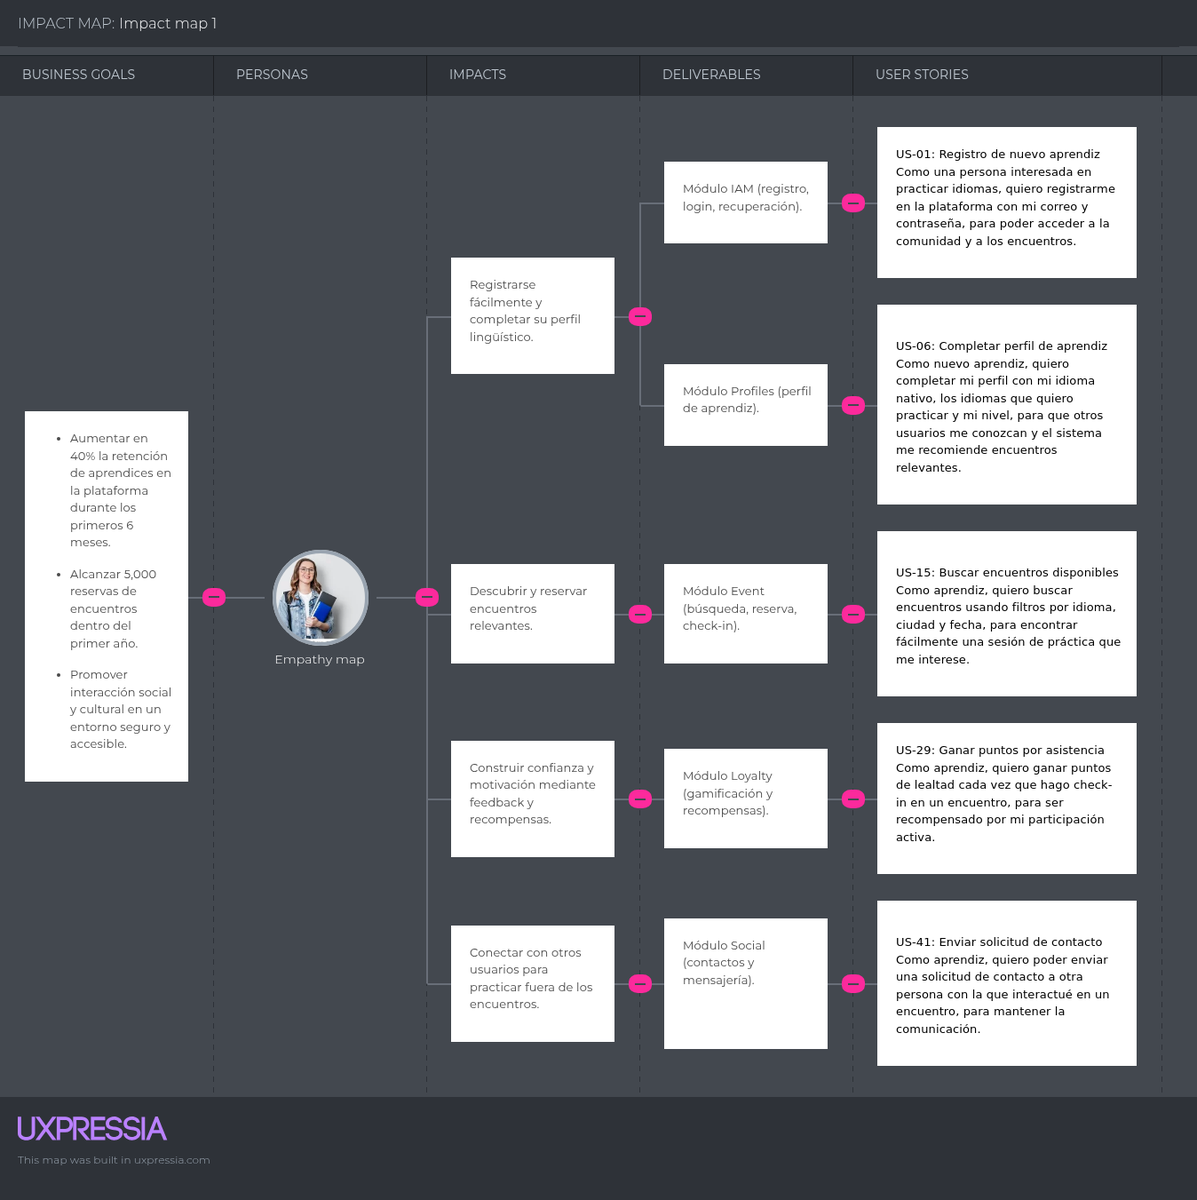
\includegraphics[keepaspectratio]{assets/img/cap3/Impact-map.png}}

\begin{center}\rule{0.5\linewidth}{0.5pt}\end{center}

\pandocbounded{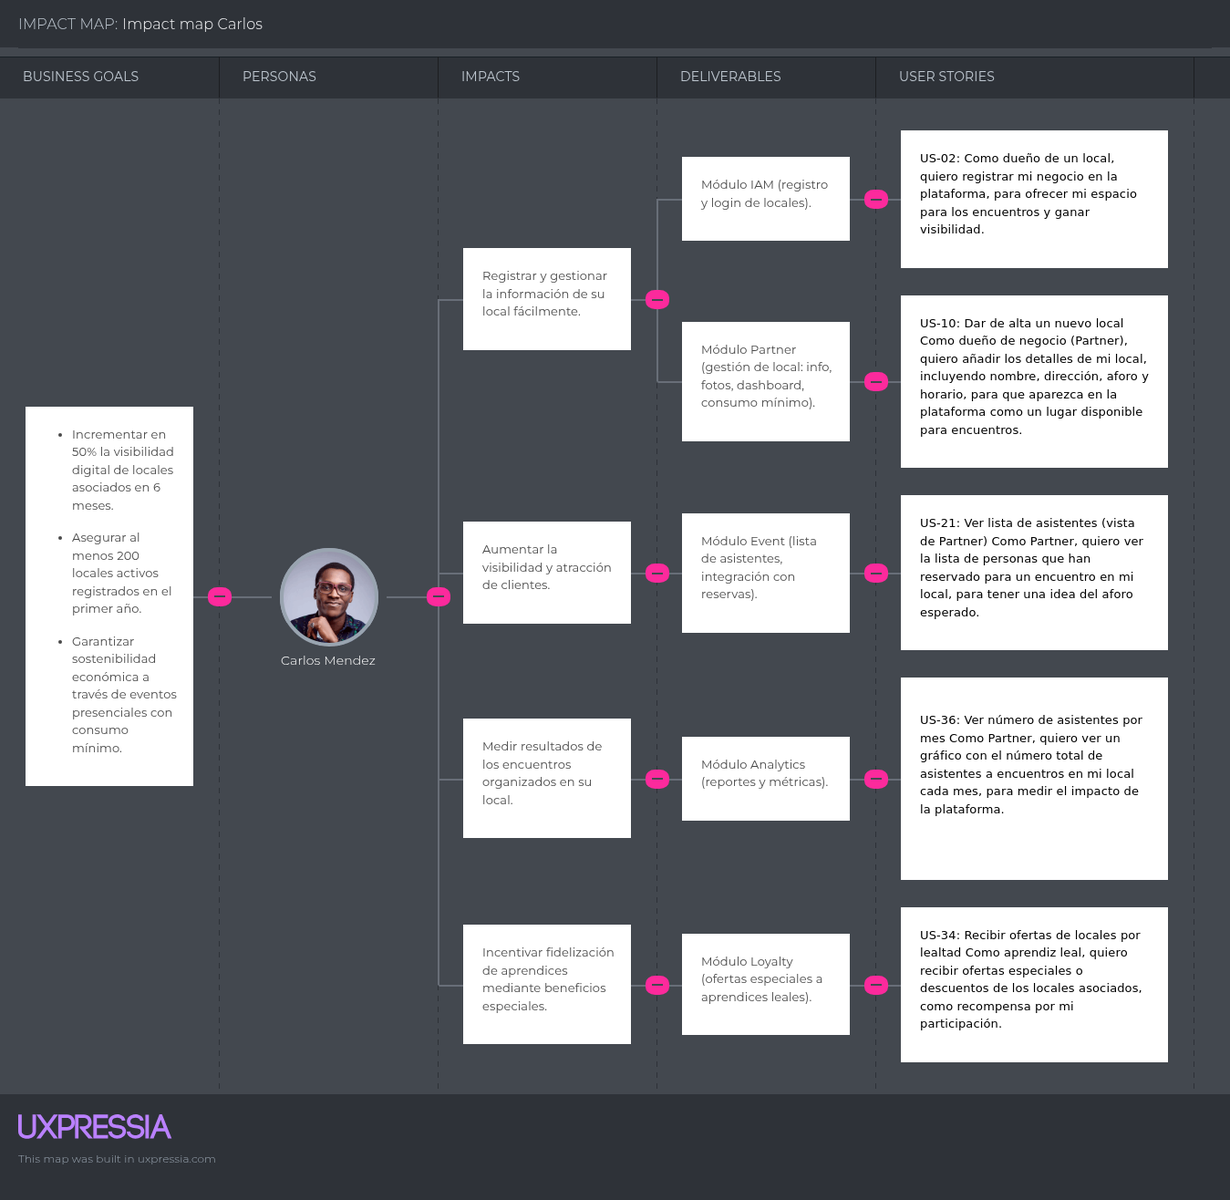
\includegraphics[keepaspectratio]{assets/img/cap3/Impact-map-Carlos.png}}

\subsection{3.4 Product
Backlog}\label{report__30-cap3-requirements-spec.md__product-backlog}

En esta sección, el equipo organiza el Product Backlog en base a su
valor para el negocio y su peso en Story Points.

{\def\LTcaptype{none} % do not increment counter
\begin{longtable}[]{@{}
  >{\raggedright\arraybackslash}p{(\linewidth - 8\tabcolsep) * \real{0.1111}}
  >{\raggedright\arraybackslash}p{(\linewidth - 8\tabcolsep) * \real{0.2593}}
  >{\raggedright\arraybackslash}p{(\linewidth - 8\tabcolsep) * \real{0.1481}}
  >{\raggedright\arraybackslash}p{(\linewidth - 8\tabcolsep) * \real{0.2222}}
  >{\raggedright\arraybackslash}p{(\linewidth - 8\tabcolsep) * \real{0.2593}}@{}}
\toprule\noalign{}
\begin{minipage}[b]{\linewidth}\raggedright
Orden
\end{minipage} & \begin{minipage}[b]{\linewidth}\raggedright
User Story Id
\end{minipage} & \begin{minipage}[b]{\linewidth}\raggedright
Título
\end{minipage} & \begin{minipage}[b]{\linewidth}\raggedright
Descripción
\end{minipage} & \begin{minipage}[b]{\linewidth}\raggedright
Story Points
\end{minipage} \\
\midrule\noalign{}
\endhead
\bottomrule\noalign{}
\endlastfoot
1 & US01 & Registro de nuevo aprendiz & Como** una persona interesada en
practicar idiomas \textbf{Quiero} registrarme en la plataforma con mi
correo y contraseña \textbf{Para} poder acceder a la comunidad y a los
encuentros. & 3 \\
2 & US03 & Inicio de sesión & \textbf{Como} usuario registrado (aprendiz
o dueño de local) \textbf{Quiero} iniciar sesión con mi correo y
contraseña \textbf{Para} acceder a mis funcionalidades personalizadas. &
3 \\
3 & US06 & Completar perfil de aprendiz & \textbf{Como} nuevo aprendiz
\textbf{Quiero} completar mi perfil con mi idioma nativo, los idiomas
que quiero practicar y mi nivel \textbf{Para} que otros usuarios me
conozcan y el sistema me recomiende encuentros relevantes. & 3 \\
4 & US15 & Buscar encuentros & \textbf{Como} aprendiz \textbf{Quiero}
buscar encuentros usando filtros por idioma, ciudad y fecha
\textbf{Para} encontrar fácilmente una sesión de práctica que me
interese. & 3 \\
5 & US16 & Ver detalles de encuentro & \textbf{Como} aprendiz
\textbf{Quiero} ver los detalles completos de un encuentro \textbf{Para}
saber el idioma, el tema, el lugar, la hora y quiénes más asistirán. &
2 \\
6 & US17 & Reservar encuentro & \textbf{Como} aprendiz \textbf{Quiero}
reservar mi cupo en un encuentro que tenga plazas disponibles
\textbf{Para} asegurar mi asistencia. & 5 \\
7 & US22 & Recordatorio de encuentro & \textbf{Como} aprendiz con una
reserva \textbf{Quiero} recibir una notificación de recordatorio 24
horas antes del encuentro \textbf{Para} no olvidarme de asistir. & 2 \\
8 & US26 & Cancelar reserva & \textbf{Como} aprendiz \textbf{Quiero}
poder cancelar mi reserva a un encuentro con antelación \textbf{Para}
liberar mi cupo si no puedo asistir. & 3 \\
9 & US27 & Historial de encuentros & \textbf{Como} aprendiz
\textbf{Quiero} tener un historial de los encuentros a los que he
asistido \textbf{Para} recordar los lugares y las fechas. & 2 \\
10 & US25 & Feedback de encuentro & \textbf{Como} aprendiz que asistió a
un encuentro \textbf{Quiero} dejar una calificación y un comentario
sobre mi experiencia \textbf{Para} ayudar a otros usuarios y a los
locales. & 3 \\
11 & US28 & Ver mapa de locales & \textbf{Como} aprendiz \textbf{Quiero}
ver locales disponibles según mi ubicación \textbf{Para} encontrar los
lugares más cercanos donde para organizar encuentros. & 5 \\
12 & US02 & Registro de nuevo local & \textbf{Como} dueño de un local
\textbf{Quiero} registrar mi negocio en la plataforma \textbf{Para}
ofrecer mi espacio para los encuentros y ganar visibilidad. & 5 \\
13 & US10 & Registrar local & \textbf{Como} dueño de negocio (Partner)
\textbf{Quiero} añadir los detalles de mi local, incluyendo nombre,
dirección, aforo y horario \textbf{Para} que aparezca en la plataforma
como un lugar disponible para encuentros. & 5 \\
14 & US13 & Definir consumo mínimo & \textbf{Como} Partner
\textbf{Quiero} tener la opción de definir un consumo mínimo sugerido
para los asistentes a encuentros en mi local \textbf{Para} asegurar un
retorno económico. & 2 \\
15 & US11 & Editar local & \textbf{Como} Partner \textbf{Quiero} poder
editar los detalles de mi local registrado \textbf{Para} mantener la
información actualizada (ej. cambio de horario). & 3 \\
16 & US12 & Añadir fotos del local & \textbf{Como} Partner
\textbf{Quiero} subir varias fotos de mi local \textbf{Para} hacerlo más
atractivo y mostrar el ambiente a los aprendices. & 3 \\
17 & US14 & Dashboard del local & \textbf{Como} Partner \textbf{Quiero}
acceder a un resumen de la actividad de mi local \textbf{Para} entender
rápidamente cuántos encuentros se han realizado y cuántas personas han
asistido. & 5 \\
18 & US36 & Ver asistentes por mes & \textbf{Como} Partner
\textbf{Quiero} conocer la cantidad de asistentes en mi local cada mes
mediante gráficos \textbf{Para} medir el impacto de la plataforma. &
5 \\
19 & US37 & Ver calificación promedio & \textbf{Como} Partner
\textbf{Quiero} ver la calificación promedio que los aprendices le han
dado a los encuentros realizados en mi local \textbf{Para} evaluar la
satisfacción del cliente. & 3 \\
20 & US29 & Ganar puntos & \textbf{Como} aprendiz \textbf{Quiero} ganar
puntos de lealtad cada vez que hago check-in en un encuentro
\textbf{Para} ser recompensado por mi participación activa. & 5 \\
21 & US30 & Ver puntos y nivel & \textbf{Como} aprendiz \textbf{Quiero}
poder ver mi saldo total de puntos y mi nivel actual en mi perfil
\textbf{Para} seguir mi progreso. & 1 \\
22 & US35 & Mantener racha & \textbf{Como} aprendiz \textbf{Quiero} que
el sistema registre mi racha de asistencia semanal \textbf{Para}
motivarme a participar de forma consistente. & 3 \\
23 & US31 & \textbf{Como} aprendiz \textbf{Quiero} desbloquear insignias
al alcanzar ciertos hitos (ej. ``Asistir a 5 encuentros de francés'')
\textbf{Para} sentir que logro algo. & 5 & \\
24 & US41 & Enviar solicitud de contacto & \textbf{Como} aprendiz
\textbf{Quiero} poder enviar una solicitud de contacto a otra persona
con la que interactué en un encuentro \textbf{Para} mantener la
comunicación. & 3 \\
25 & US42 & Aceptar solicitudes & \textbf{Como} aprendiz \textbf{Quiero}
recibir notificaciones de nuevas solicitudes de contacto \textbf{Para}
poder aceptarlas o rechazarlas. & 3 \\
26 & US43 & Ver contactos & \textbf{Como} aprendiz \textbf{Quiero} tener
una lista de todos los usuarios con los que he conectado \textbf{Para}
poder iniciar una conversación. & 2 \\
27 & US44 & Enviar mensajes & \textbf{Como} aprendiz \textbf{Quiero}
poder enviar un mensaje directo a uno de mis contactos \textbf{Para}
organizar una futura práctica de idiomas. & 5 \\
28 & US45 & Notificaciones de mensajes & \textbf{Como} usuario
\textbf{Quiero} recibir una notificación cuando uno de mis contactos me
envía un mensaje \textbf{Para} poder responder a tiempo. & 5 \\
29 & US08 & Ver perfil de otros usuarios & \textbf{Como} aprendiz
\textbf{Quiero} ver el perfil de otros asistentes a un encuentro
\textbf{Para} conocer sus idiomas de interés y conectar con ellos. &
2 \\
30 & US07 & Editar perfil & \textbf{Como} aprendiz \textbf{Quiero} poder
editar la información de mi perfil en cualquier momento \textbf{Para}
mantenerla actualizada. & 2 \\
31 & US09 & Subir foto de perfil & \textbf{Como} usuario \textbf{Quiero}
subir una foto de perfil \textbf{Para} personalizar mi cuenta y que
otros me reconozcan más fácilmente. & 2 \\
32 & US46 & Reportar usuario & \textbf{Como} usuario \textbf{Quiero}
tener la opción de reportar a otro usuario por comportamiento
inapropiado \textbf{Para} mantener un ambiente seguro y respetuoso en la
comunidad. & 5 \\
33 & US47 & Dashboard admin & \textbf{Como} administrador de la
plataforma \textbf{Quiero} acceder a información sobre el uso que se le
da a la plataforma en mi local \textbf{Para} monitorear su buen
funcionamiento. & 8 \\
34 & US48 & Gestionar usuarios & \textbf{Como} administrador
\textbf{Quiero} poder ver la lista de todos los usuarios y poder
desactivar una cuenta en caso de abuso \textbf{Para} mantener la calidad
de la comunidad. & 5 \\
35 & US49 & Validar locales & \textbf{Como} administrador
\textbf{Quiero} tener un proceso para validar y aprobar los nuevos
locales que se registran \textbf{Para} asegurar que son lugares
apropiados y reales. & 5 \\
36 & US50 & Gestionar reportes & \textbf{Como} administrador
\textbf{Quiero} ver una lista de todos los reportes enviados por los
usuarios \textbf{Para} poder investigarlos y tomar acciones. & 8 \\
37 & US51 & Comunicación global & \textbf{Como} administrador
\textbf{Quiero} poder enviar notificaciones o correos electrónicos a
todos los usuarios \textbf{Para} comunicar novedades o mantenimientos de
la plataforma. & 8 \\
38 & US18 & Confirmación con QR & \textbf{Como} aprendiz \textbf{Quiero}
recibir una confirmación de mi reserva \textbf{Para} poder hacer
check-in fácilmente al llegar al local. & 5 \\
39 & US20 & Check-in con QR & \textbf{Como} aprendiz \textbf{Quiero}
confirmar mi asistencia a un encuentro \textbf{Para} para registrar mi
participación y recebir los beneficios por ello. & 8 \\
40 & US23 & Lista de espera & \textbf{Como} aprendiz \textbf{Quiero}
unirme a una lista de espera si un encuentro está lleno \textbf{Para}
tener la oportunidad de asistir si alguien cancela. & 3 \\
41 & US24 & Notificación de cupo & \textbf{Como} aprendiz en una lista
de espera \textbf{Quiero} recibir una notificación inmediata si un cupo
se libera \textbf{Para} poder reservarlo rápidamente. & 5 \\
42 & US04 & Cierre de sesión & \textbf{Como} usuario autenticado
\textbf{Quiero} poder cerrar mi sesión \textbf{Para} proteger la
privacidad de mi cuenta en dispositivos compartidos. & 1 \\
43 & US05 & Recuperación de contraseña & \textbf{Como} usuario
registrado \textbf{Quiero} solicitar un enlace para restablecer mi
contraseña si la he olvidado \textbf{Para} poder recuperar el acceso a
mi cuenta. & 2 \\
44 & US38 & Ver horas pico & \textbf{Como} Partner \textbf{Quiero} ver
un reporte que me muestre qué días de la semana y a qué horas se
realizan más encuentros en mi local \textbf{Para} optimizar mi personal.
& 8 \\
45 & US39 & Clientes nuevos vs recurrentes & \textbf{Como} Partner
\textbf{Quiero} saber qué porcentaje de los asistentes son nuevos
clientes versus personas que ya han venido antes \textbf{Para} medir la
captación de nuevo público. & 8 \\
46 & US40 & Descargar reportes & \textbf{Como} Partner \textbf{Quiero}
poder descargar un resumen la información de mi actividad en un formato
que pueda usar fuera de la plataforma \textbf{Para} mis registros
internos. & 5 \\
\end{longtable}
}

\begin{center}\rule{0.5\linewidth}{0.5pt}\end{center}

\pandocbounded{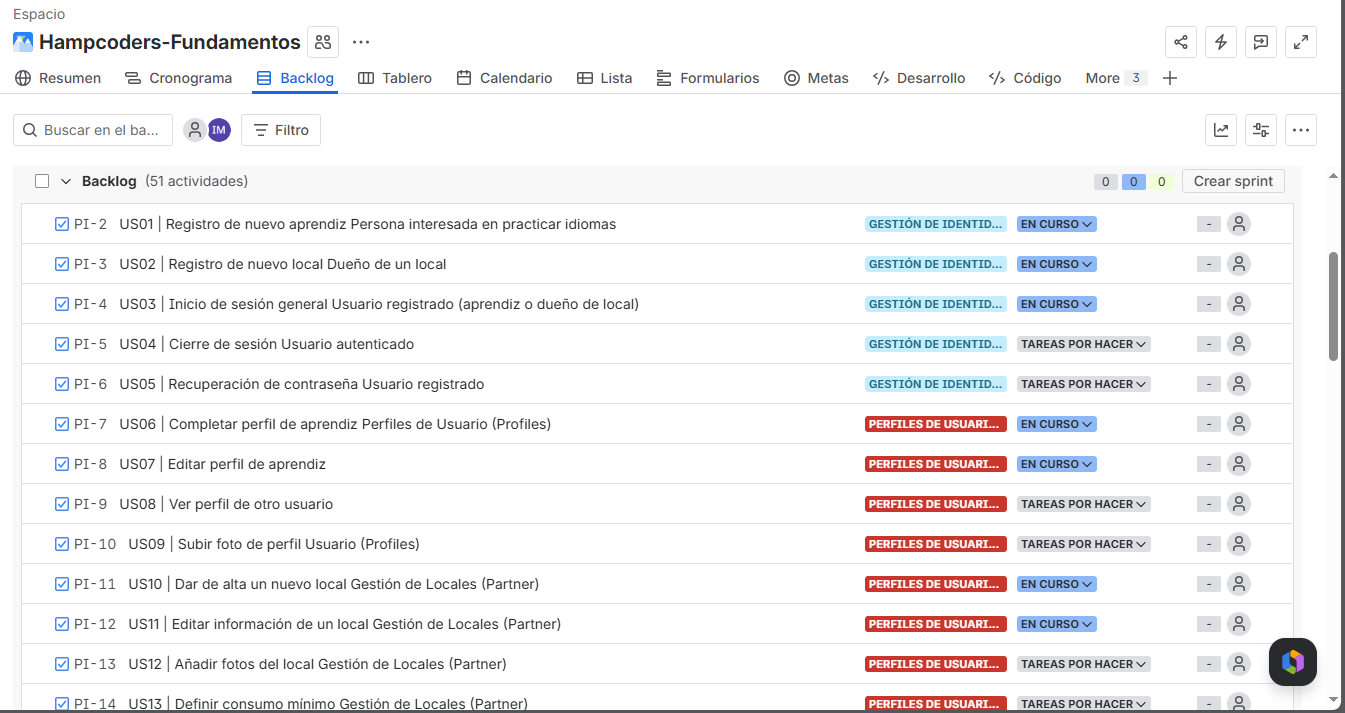
\includegraphics[keepaspectratio]{assets/img/cap3/Product-Blackog.png}}

\href{https://upc-hampcoders-fundamentos.atlassian.net/jira/software/projects/PI/boards/2/backlog?atlOrigin=eyJpIjoiNjI0Njg0NzE3MDRlNGNjOWE5ODM3ODhmMWQ2YjA5NDYiLCJwIjoiaiJ9}{Ver
Product Backlog en Jira}

\section{Conclusiones}\label{report__90-conclusiones.md__conclusiones}

\section{Referencias
Bibliografícas}\label{report__91-bibliografia.md__referencias-bibliografuxedcas}

Carrillo-García, M. E., Cascales-Martínez, A., \& Valero, A. L. (2018).
Apps para el aprendizaje de idiomas en la Universidad de Murcia. Revista
de Educación a Distancia (RED), (58).
https://revistas.um.es/red/article/view/351511/

Palma, D. G. D., \& Vázquez, M. E. M. (2023). Uso de aplicaciones
móviles como herramienta de apoyo en el aprendizaje del idioma inglés.
Ciencia Latina Revista Científica Multidisciplinar, 7(4), 2773-2788.
https://ciencialatina.org/index.php/cienciala/article/view/7139/

Cobos Guillén, C. G. (2023). Azuay Café: propuesta de una escuela
cafetería en base de la metodología del aprender haciendo para las
prácticas preprofesionales de los estudiantes de una carrera de turismo
(Master's thesis, Universidad del
Azuay).https://dspace.uazuay.edu.ec/handle/datos/13362/

Dueñas-Mendoza, A. S., \& Zaldumbide-Peralvo, D. A. Estrategias de
marketing digital para cafeterías-restaurantes en Esmeraldas, Ecuador.
Obtenido de, 593. https://www.academia.edu/download/117711219/2011.pdf/
